% !TeX encoding = windows-1252
% !TeX spellcheck = de_DE
\documentclass{scrartcl}
%%%%%%%%%%%%%%%%%%%%%%%%%%%%%%%%%%%%%%%%%%%%%%%%%%%%%%%%%%%%%%%%%%%%%%%%%%%%%%%%%%%%%%%%%%%%%%%%%%%%%%%%%%%%%%%%%%%%%%%%%%%%%%%%%%%%%%%%%%%%%%%%%%%%%%%%%%%%%%%%%%%%%%%%%%%%%%%%%%%%%%%%%%%%%%%%%%%%%%%%%%%%%%%%%%%%%%%%%%%%%%%%%%%%%%%%%%%%%%%%%%%%%%%%%%%%
\usepackage[ngerman]{babel}
\usepackage[utf8]{inputenc}
\usepackage[T1]{fontenc}
\usepackage{ae,aecompl}
\usepackage[a4paper,bottom=1in,top=1in]{geometry}
\usepackage{amssymb,amsmath,amsfonts}
\usepackage{csquotes}
\usepackage{pdfsync}
\usepackage{enumerate}
\usepackage{graphicx}
\usepackage{qtree}
\usepackage{pdfpages}
\newenvironment{rcases}{%
  \left.\renewcommand*\lbrace.%
  \begin{cases}}%
{\end{cases}\right\rbrace}

\usepackage{hyperref}
\hypersetup{
pdfauthor={Willi Mutschler},
pdftitle={FAG: Marko Anschrift},
pdfsubject={},
pdfproducer={LaTeX},
colorlinks=false,  pdfborder={0 0 0},     pdfstartview={FitH},   plainpages = false, }
\usepackage{fancyhdr}
\pagestyle{fancy}
\lhead{\small FAG: Makro\"{o}konomik Anschrift (Willi Mutschler)}
\begin{document}
\section{VGR}
\subsection{Verst\"{a}ndnis (30 Min)}
\begin{itemize}
\item Prinzip: Wie gro{\ss} ist der Kuchen? H\"{o}he des Bruttoinlandsprodukts!
\item Entstehung: Wodurch wurde der Kuchen generiert?\\ Gesamte Wertsch\"{o}pfung, Summe aller Mehrwerte
\item Verwendung: Was wird mit den Kuchenst\"{u}cken gemacht?\\ Konsum, Ersparnis, Investitionen, Exporte, Importe
\item Verteilung: Wer erh\"{a}lt etwas vom Kuchen?\\ Volkseinkommen: L\"{o}hne, Gewinne
\item Vokabular:
    \begin{itemize}
      \item Stromgr\"{o}{\ss}en: Einkommen, Konsum, Investitionen, Abschreibungen, Gewinn, Geburten, Sterbef\"{a}lle\\ (\emph{pro} Periode, \textbf{Zeitraumbezogen})
      \item Bestandsgr\"{o}{\ss}en: Verm\"{o}gen, Kapitalstock, Bev\"{o}lkerungszahl, Arbeitslosigkeit, Geldmenge\\ (\emph{in} Periode, \textbf{Zeitpunktbezogen})
    \end{itemize}
\item Sektoren/Akteure
    \begin{itemize}
      \item Haushalte: erbringen Faktorleistungen, konsumieren und sparen
      \item Unternehmen: produzieren und verkaufen Waren und Dienstleistungen, zahlen L\"{o}hne und Gewinne, investieren und verschulden sich
      \item Staat: Staatskonsum, Staatsinvestitionen, Steuern, Subventionen, Transfers
      \item Ausland (\"{u}brige Welt): Export/Import von Waren, Dienst- und Faktorleistungen
    \end{itemize}
\item Wichtigstes Prinzip: Angebot $=$ Nachfrage:
    \begin{align*}
      \underbrace{Y+IM}_\text{Angebot} &= \underbrace{C+I+G+EX}_\text{Nachfrage}
    \end{align*}
    Zentraler Unterschied offene vs. geschlossene Volkswirtschaft:\\
    Gesamtwirtschaftliche inl\"{a}ndische Nachfrage muss nicht gleich dem inl\"{a}ndischem Angebot an G\"{u}tern und Dienstleistungen sein! G\"{u}ter k\"{o}nnen vom Ausland importiert bzw. ins Ausland exportiert werden. Zahlungsbilanz erfasst alle Transaktionen zwischen Inl\"{a}ndern und Ausl\"{a}ndern. Wir betrachten also folgenden Au{\ss}enbeitrag (Leistungsbilanz) und Finanzierungssaldo
    \begin{align*}
      Lb = \underbrace{EX-IM}_\text{Nettoexporte} = \underbrace{(Y - C - T)}_{S_{Pr}} + \underbrace{(T-G)}_{S_{St}} - I_{Pr} - I_{St}= \underbrace{S-I}_\text{Nettokapitalablfl\"{u}sse} =FS
    \end{align*}
    Hinweis: Formel $FS=Einnahmen-Ausgaben=S-I$ ist immer Finanzierungssaldo, entweder f\"{u}r Volkswirtschaft gesamt oder einzelne Akteure.
    \begin{itemize}
      \item $EX-IM$ ist internationaler G\"{u}terstrom, $S-I$ ist internationaler Finanzstrom
      \item $EX>IM$ Leistungsbilanz\"{u}berschuss, $S>I$ Nettodarlehensgeber
      \item $EX<IM$ Leistungsbilanzdefizit, $S<I$ Nettodarlehensnehmer
    \end{itemize}
    Ein Leistungsbilanz-Defizit erfordert einen Kapitalzufluss zur Finanzierung der Nettoimporte!
\item Was h\"{a}ngt wie zusammen?
    \begin{align*}
    &\text{\textbf{Entstehungsrechnung}:}\\
      BIP&= \overbrace{\underbrace{PW}_\text{Produktionswert} - \underbrace{V}_\text{Vorleistungen}}^\text{Bruttowertsch\"{o}pfung} + \underbrace{T_G}_\text{G\"{u}tersteuern} - \underbrace{SUB_G}_\text{G\"{u}tersubventionen} \\
    &\text{\textbf{Verwendungsrechnung}:}\\
      BIP &= (C_{pr} + C_{St}) + (I_{br,pr}+I_{br,St}) + EX-IM \qquad \Rightarrow \text{FOKUS INLAND}\\
      BNE &= BIP +  \underbrace{\text{Saldo Prim\"{a}reinkommen Welt}}_{+\text{Inl\"{a}nder im Ausland}-\text{Ausl\"{a}nder im Inland}} \qquad \Rightarrow \text{FOKUS INL\"{A}NDER}\\
      NNE &= BNE - ABS\\
&\text{\textbf{Verteilungsrechnung}:}\\
      \underbrace{Y}_\text{Volkseinkommen} &= NNE - \underbrace{\underbrace{T_{ind}}_\text{ind. Steuern}}_{Mehrwertsteuer, Okosteuer, Alkohol, Tabak, Gewerbe, Strom} + \underbrace{SUB}_\text{Unt-Subventionen}\\
      \underbrace{Y}_\text{Volkseinkommen} & = \underbrace{W}_\text{ANEntgelt} + \underbrace{Q}_\text{Untern.undVerm\"{o}gens.EK}\\
      \underbrace{Y^V}_\text{Verf\"{u}gbares EK} &= NNE + \underbrace{SLU}_\text{Saldo lauf. \"{U}bertragungen (+aus \"{U}W -in \"{U}W)} = C + S
    \end{align*}
    (SLU: Die \"{U}bertragungsbilanz h\"{a}lt die geleisteten und empfangenen privaten und \"{o}ffentlichen \"{U}bertragungen, wie \"{U}berweisungen von ausl\"{a}ndischen Arbeitnehmern in ihre Heimatl\"{a}nder, Beitr\"{a}ge an internationale Organisationen und die Entwicklungshilfe fest. Allgemein gesagt erfasst sie den unentgeltlichen Transfer zwischen In- und Ausland.)
\item Wichtige Konzepte:
    \begin{itemize}
        \item Inlandskonzept: Produktion innerhalb Grenzen, unabh\"{a}ngig von wem ($\hookrightarrow$ BIP)
        \item Inl\"{a}nderkonzept: Durch Inl\"{a}nder get\"{a}tigte Produktion bzw. erzieltes Einkommen, unabh\"{a}ngig ob im Inland oder Ausland ($\hookrightarrow$ BNE)
      \end{itemize}
\item Was ist das BIP: Bruttoinlandsprodukt (BIP) gibt die (j\"{a}hrliche) Wertsch\"{o}pfung als Gesamtwert aller G\"{u}ter (abz\"{u}glich Vorleistungen) an, die innerhalb der Landesgrenzen einer Volkswirtschaft hergestellt wurden.
\item Welches der Einkommenskonzepte ist besonders aussagekr\"{a}ftig?\\
Antwort h\"{a}ngt von der konkreten Fragestellung ab:\\
BIP: Gutes Ma{\ss} f\"{u}r gesamtwirtschaftliche Produktion im Inland (und daher von Interesse bei der Analyse von Konjunkturschwankungen).\\
BNE: relevantes Ma{\ss} f\"{u}r das Einkommen der Inl\"{a}nder.\\
NNE: besserer Indikator f\"{u}r den Lebensstandard der Inl\"{a}nder, da es um Abschreibungen korrigiert.\\
Volkseinkommen bzw. verf\"{u}gbare Einkommen der privaten HH: sind wiederum bessere Indikatoren falls die Steuerbelastung die Versorgung mit \"{o}ffentlichen G\"{u}tern nicht angemessen abbildet.
%\item BIP als Wohlstandsindikator:\\
%Bewertung \"{o}ffentlicher G\"{u}ter Verwaltungsleistungen des \"{o}ffentlichen Sektors werden zu Herstellungskosten bewertet. Aus den Aufwendungen f\"{u}r Bildungseinrichtungen, das Gesundheitssystem und die Justiz kann aber nicht auf die Qualit\"{a}t oder den Wert dieser Einrichtungen geschlossen werden.\\
%Markttransaktionen und Haushaltsproduktion BIP erfasst ausschlie{\ss}lich Markttransaktionen. Aktivit\"{a}ten wie die Reinigung der Wohnung, die Kinderbetreuung oder Gartenarbeit werden nur ber\"{u}cksichtigt, wenn sie steuerlich deklariert worden sind. In allen F\"{a}llen, wo dies nicht der Fall ist (z.B. Produktion im privaten Haushalt), ist die Wirtschaftsleistung h\"{o}her als vom BIP ausgewiesen. Die international unterschiedliche Bedeutung dieser Aktivit\"{a}ten erschwert dabei die Vergleichbarkeit von BIP-Daten.\\
%Umwelteffekte des BIP-Wachstums Wirtschaftsaktivit\"{a}t kann sich negativ auf Umweltfaktoren (Luft, Wasser oder Boden) auswirken. Im BIP werden aber nur die positiven Produktionseffekte ber\"{u}cksichtigt. Die resultierende Umweltbelastung und die damit einhergehende Beeintr\"{a}chtigung der Lebensqualit\"{a}t haben hingegen keinen Einfluss auf das BIP.\\
%BIP pro Kopf und Einkommensverteilung BIP pro Kopf ist eine Durchschnittsgr\"{o}{\ss}e. Bei ungleicher Einkommensverteilung (hoher Gini-Koeffizient) kann aus einem BIP-Wachstum nicht geschlossen werden, dass die Mehrheit der Bev\"{o}lkerung davon profitiert.\\
%Nachhaltigkeit des BIP Betrifft das Wohlstandspotenzial k\"{u}nftiger Generationen. Zuk\"{u}nftiges BIP sollte mindestens so hoch sein wie sein aktuelles Niveau. Wirtschaftswachstum kann eventuell nicht nachhaltig sein, wenn es auf einem intensiven Verbrauch ersch\"{o}pfbarer nat\"{u}rlicher Ressourcen basiert.
%Nicht-\"{o}konomische Gr\"{o}{\ss}en F\"{u}r den Wohlstand relevante Gr\"{o}{\ss}en wie politische Freiheit und soziale Sicherheit werden ebenfalls nicht im BIP erfasst.\\
%BIP und Freizeitkonsum Ein geeigneter Wohlstandsindikator m\"{u}sste den Parameter Freizeit enthalten, da dieser zur Lebensqualit\"{a}t beitr\"{a}gt. Wird in einer Volkswirtschaft mehr Arbeitsinput geleistet, so steigt das BIP, nicht notwendigerweise aber auch der Wohlstand.
\end{itemize}
\subsection{Einfache Berechnungen (10 Min)}
\begin{align*}
  BIP &= PW - V + T_G - SUB_G = 5000 - 2700 + 580 - 30 = 2850\\
  LB &= EX - IM = BIP - C_{Pr} - C_{St} - I_{Br} = 2850 - 1000 - 500 - 870 = 480\\
  EX &= LB + IM = 480 + 770 = 1250\\
  I_{netto} &= I_{Br} - ABS = 870-450=420\\
  BNE &= BIP + Saldo PEK = 2850 - 40 = 2810\\
  NNE &= BNE - ABS = 2810 - 450 = 2360
\end{align*}
\subsection{Verst\"{a}ndnisfragen (15 Min)}
\begin{enumerate}
  \item $NNE=BNE - ABS$ (wahr)
  \item $S=Y-C$ alles Stromgr\"{o}{\ss}en! (falsch)
  \item $S-I = EX-IM >0$ (wahr)
  \item $NWS = BWS -ABS, ABS>NWS, BWS = NWS + AB >0$ (falsch)
  \item Dies ist die Definition (wahr)
  \item Geschlossene Volkswirtschaft: $S=I$ Finanzierungssaldo: $FS=-S+I = 0$ (wahr)\\
  Warum Finanzierung: $S_H + S_U + S_{St} = I_{U}+I_{St} \Leftrightarrow S_H + (S_U-I_U)+(S_{St}-I_{St})=0$
  \item $NIP = BIP-ABS, NNE = BIP + SPEK -ABS,\\ NNE < NIP \Leftrightarrow BIP +SPEK - ABS < BIP -ABS \Leftrightarrow SPEK < 0 \rightarrow $ m\"{o}glich! (falsch)
  \item $YV = NNE + SLUW$ (falsch)
  \item falsch.
  \item $NNE=BIP+SPEK-ABS, NNE-BIP<0 \leftrightarrow SPEK < ABS$ m\"{o}glich! (falsch)
  \item Verteilung des \textbf{EINKOMMENS} auf L\"{o}hne und Gewinne! (falsch)
  \item $I_{netto} = I_{br} - ABS$. Wenn Bruttoinvestitionen unterbleiben und gleichzeitig der Kapitalbestand an Wert verliert, ist $I_{netto}<0$ m\"{o}glich. Die Bruttoinvestition ist entweder positiv oder gleich Null, denn eine Volkswirtschaft kann nicht weniger als nichts investieren! (falsch)
  \item $S-I<0$, es muss Kapital importiert werden um Investitionen zu finanzieren (wahr)
  \item $S-I^{br} = S - I^{ne} -ABS$, f\"{u}r ABS=0 gilt $S=I^{ne}$
  \item $I_{br} = I_{netto} + ABS, I_{br} > ABS \leftrightarrow I_{netto} > 0$ (falsch)
  \item $S-I = EX-IM = 0$ (wahr)
  \item wahr, da geschlossene Volkswirtschaft! $I=S$!
\end{enumerate}

\subsection{Lohnquote}
\begin{align*}
  Unber.LQ = \frac{Y^{AN}}{NNE}
\end{align*}
$Y^{AN}:$ Bruttol\"{o}hne + AG-Beitr\"{a}ge = 1100+300 = 1400\\
$NNE$: BNE-AB = 2000 - 300 = 1700 \\
Unber.LQ = 1400/1700 = 0.82
\begin{enumerate}[a)]
  \item Anteil Selbst\"{a}ndiger $\uparrow$, c.p. $Y^{AN} \downarrow \rightarrow LQ \downarrow$
  \item Kein Effekt, da AN-Beitr\"{a}ge nur Aufteilung von Bruttol\"{o}hnen auf AN und Sozialversicherung betreffen.
  \item Kein Effekt, Konsum spielt auf der Verwendungsseite eine Rolle, nicht hier auf der Verteilungsseite!
\end{enumerate}

\subsection{Gini-Koeffizient}
\begin{tabular}{ccccc}
  Person i & EK $x_i$ & Summe $x_i$ & $u_i=\frac{i}{n}$ & $v_i=\frac{\sum_{j=1}^i x_j}{\sum_{j=1}^n x_j}$ \\
  1 & 1 & 1 & 1/10 & 1/20 \\
  2 & 1 & 2 & 2/10 & 2/20 \\
  3 & 1 & 3 & 3/10 & 3/20 \\
  4 & 1 & 4 & 4/10 & 4/20 \\
  5 & 1 & 5 & 5/10 & 5/20 \\
  6 & 3 & 8 & 6/10 & 8/20 \\
  7 & 3 & 11 & 7/10 & 11/20 \\
  8 & 3 & 14 & 8/10 & 14/20 \\
  9 & 3 & 17 & 9/10 & 17/20 \\
  10 & 3 & 20 & 10/10 & 20/20
\end{tabular}
\begin{center}
  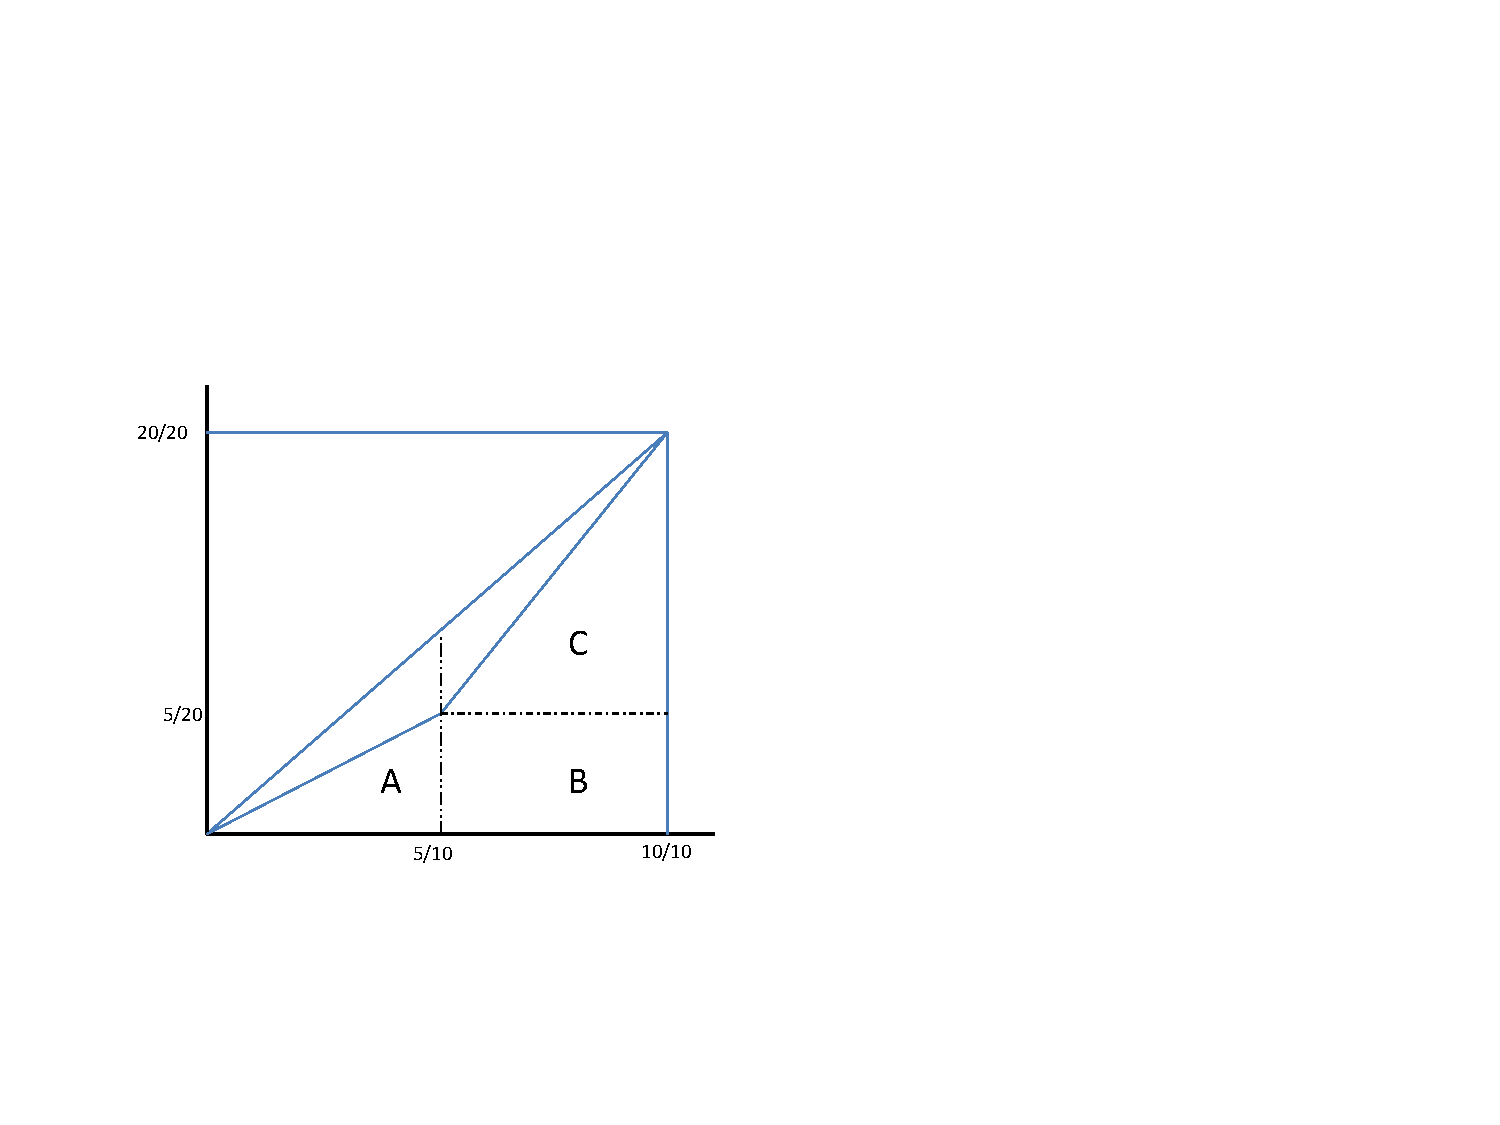
\includegraphics[width=0.5\textwidth]{Bilder/lorenz.pdf}
\end{center}
Gini-Koeffizient ist (Fl\"{a}che zwischen Diagonalen und Lorenzkurve) geteilt durch Fl\"{a}che der Diagonalen
\begin{align*}
  G = \frac{0.5\cdot 1\cdot1 - (\underbrace{0.5\cdot 5/10 \cdot 5/20}_{A} + \underbrace{5/10\cdot5/20}_B + \underbrace{0.5\cdot 5/10 \cdot 15/20)}_{C}}{0.5\cdot1\cdot 1}
  = \frac{1}{4}
\end{align*}


\subsection{BIP-Konzepte: Nominal, Real, Kettenindex}
\begin{enumerate}[a)]
\item Das nominale BIP ist die Summe aller verkauften Endprodukte, bewertet zu den jeweiligen Preisen, d.h. zu den Preisen der gerade
betrachteten Periode. Das nominale BIP kann aus zwei Gr\"{u}nden zunehmen: i) Die Produktion der meisten G\"{u}ter nimmt im Zeitablauf zu. ii) Aber auch die Preise der meisten G\"{u}ter steigen.
Um den Mengeneffekt der Produktion zu isolieren, m\"{u}ssen wir den Effekt steigender Preise herausrechnen: Das reale BIP ist das Ma{\ss} der VGR f\"{u}r die Menge der gesamtwirtschaftlichen
Produktion. Es bereinigt das nominale BIP um Preissteigerungen.\\
Wie berechnet man das reale BIP?
Alte Praxis des Statistischen Bundesamtes: Benutze die Preise eines Basisjahrs. Dieses Basisjahr wurde alle 5 Jahre aktualisiert und die
Zeitreihe des realen BIP neu berechnet.\\
Seit 2005: Kettenindexverfahren: Zur Berechnung des realen BIP-Wachstums zwischen zwei aufeinanderfolgenden Jahren werden jeweils die Preise des Vorjahres verwendet (und alle so gewonnenen Wachstumsraten zu
einem Index verkettet).
  \item \begin{align*}
  2005&: 2224 \cdot \frac{100}{100} = 2224\\
  2006&: 2231 \cdot \frac{103,7}{100} = 2313,55\\
  2007&: 2267 \cdot \frac{107,1}{100} = 2427,96
  \end{align*}
  \item \begin{align*}
    2005-2006&: (2231/2224-1)\cdot 100\% = 0,31 \%\\
    2006-2007&: (2267/2231-1)\cdot 100\% = 1,61 \%
  \end{align*}
  \item \begin{align*}
    (2267/2224-1)\cdot 100\% = (1,019 -1)\cdot 100\% = 1,93 \%
  \end{align*}
  \item \begin{align*}
    \sqrt{1,0031\cdot1,0161} -1 = 0.96\%\\
    \sqrt{1,019}-1 = 0.95\%
  \end{align*}
\end{enumerate}
%\section{Die Klassisch-Neoklassische Theorie}
%\subsection{Verst\"{a}ndnis}
%\begin{enumerate}
%  \item Erl\"{a}uterungen:
%  \begin{itemize}
%  \item \textbf{Das repr\"{a}sentative Unternehmen:}
%  \begin{itemize}
%    \item ist eine gedachte Durchschnittseinheit, die sich - bis auf die Gr\"{o}{\ss}enordnung - so verh\"{a}lt, wie der Unternehmenssektor insgesamt.
%    \item Gewinnmaximierungskalk\"{u}l: Das repr\"{a}sentative Unternehmenproduziert verh\"{a}lt sich als Mengenanpasser. Es prouziert G\"{u}ter Y mit Arbeitseinsatz N und Kapital K gem\"{a}{\ss} einer Produktionsfunktion $Y=F(N,K)$ mit $F_N,F_K >0$ und $F_{NN},F_{KK}<0$. Oft ist $F$ vom Typ Cobb-Douglas: $Y=A N^{\alpha} K^{1-\alpha}$. Eine Arbeitseinheit kostet $W$ [Euro], eine Einheit Kapital wird zum Nominalzins $R$ gemietet und eine G\"{u}tereinheit wird zum Preis $P$ [Euro] verkauft. Das Repr\"{a}sentative Unternehmen ist ein Mengenanpasser, d.h. es nimmt das Preisniveau P, den Nominallohn W und den Zins R als gegeben an und w\"{a}hlt die Mengen N und K, um seinen Gewinn zu maximieren. Somit herrscht vollst\"{a}ndige Konkurrenz, das das Repr\"{a}sentative Unternehmen P, W oder R nicht beeinflussen kann. Formal:
%        \begin{align*}
%          \Pi = P \cdot Y - W \cdot N - R \cdot K
%        \end{align*}
%    \item Im Optimum gilt, dass die Wertgrenzprodukte von Arbeit und Kapital gleich ihrer Entlohnung sein m\"{u}ssen, formal:
%        \begin{align*}
%          \frac{\partial \Pi}{\partial N} &= \overbrace{P \frac{\partial Y}{\partial N}}^{\text{Wertgrenzprodukt}} - W \overset{!}{=} 0 \leftrightarrow \overbrace{\frac{\partial Y}{\partial N}}^\text{Grenzprodukt} = \overbrace{\frac{W}{P}}^\text{Reallohn} \\
%          \frac{\partial \Pi}{\partial K} &= \underbrace{P \frac{\partial Y}{\partial K}}_\text{Wertgrenzprodukt} - R \overset{!}{=} 0 \leftrightarrow \underbrace{\frac{\partial Y}{\partial K}}_\text{Grenzprodukt} = \underbrace{\frac{R}{P}}_\text{Realzins}
%        \end{align*}
%    \item Arbeitsnachfrage ist das Umstellen von der ersten Optimalit\"{a}tsbedingung nach N. Zum Beispiel f\"{u}r Cobb-Douglas-PF:
%        \begin{align*}
%          \frac{\partial Y}{\partial N} &= A \alpha N^{\alpha-1}K^{1-\alpha} =\frac{W}{P}\\
%          N &= \left(\frac{W}{P}\right)^\frac{1}{\alpha-1} \left(\frac{1}{A \alpha}\right)^\frac{1}{\alpha-1} \left(\frac{1}{K^{1-\alpha}}\right)^\frac{1}{\alpha-1} =  \left(\frac{\alpha A}{\frac{W}{P}}\right)^{\frac{1}{1-\alpha}}K \equiv N^d
%          \end{align*}
%    \item Zusammenhang mit Reallohn: Allgemein:
%    \begin{align*}
%      \frac{\partial(W/P)}{\partial N} = \frac{\partial Y^2}{\partial N \partial N}= \underbrace{F_{NN}}_\text{lt.Annahme} <0
%    \end{align*}
%    Konkret f\"{u}r Cobb-Douglas-PF:
%          \begin{align*}
%          \frac{\partial N^d}{\partial \frac{W}{P}} &= \underbrace{\frac{1}{\alpha-1}}_{<0} \left(\frac{W}{P}\right)^{\frac{1}{\alpha-1}-1} \left(\frac{1}{A \alpha}\right)^\frac{1}{\alpha-1} \left(\frac{1}{K^{1-\alpha}}\right)^\frac{1}{\alpha-1} <0
%        \end{align*}
%        Grund f\"{u}r negative Ableitung: Je h\"{o}her der Reallohn ist, desto gr\"{o}{\ss}er muss das Grenzprodukt der Arbeit sein, damit der Grenzerl\"{o}s gr\"{o}{\ss}er als die Grenzkosten ist. Da bei zus\"{a}tzlichen Arbeitseinheiten der Grenzerl\"{o}s abnimmt h\"{a}ngt die Nachfrage des Unternehmens nach Arbeit negativ vom Reallohn ab.
%  \end{itemize}
%  \item \textbf{Der repr\"{a}sentative Haushalt:}
%  \begin{itemize}
%    \item Analog zum RU ist der RHH eine gedachte Durchschnittseinheit, die sich - bis auf die Gr\"{o}{\ss}enordnung - so verh\"{a}lt wie der Haushaltssektor insgesamt. Der Haushalt maximiert seinen Nutzen aus Konsum und Freizeit, d.h. er entscheidet \"{u}ber seinen Konsum und sein Arbeitsangebot gegeben seines Einkommens. Annahmegem\"{a}{\ss} ist er der Besitzer der Unternehmen und vermietet Kapital an diese. Formal gilt folgende Budgetrestriktion
%        \begin{align*}
%          \underbrace{P C}_\text{Konsum} + \underbrace{P S}_\text{Ersparnis} = \underbrace{WN^s}_\text{Lohn-EK} + \underbrace{\Pi}_\text{Gewinne} + \underbrace{\Omega}_\text{Kapital-EK}
%        \end{align*}
%    \item Arbeitsangebot: erfolgt derart, dass der gr\"{o}{\ss}te Nutzen aus der Kombination von Arbeit gezogen wird, formal:
%    \begin{align*}
%      N^s = N^s\overset{+}{\left(\frac{W}{P}\right)} \overset{\text{z.B.}}{=} b \left(\frac{W}{P}\right)^\gamma, \quad \text{mit } b,\gamma >0
%    \end{align*}
%    Das Arbeitsangebot ist positiv abh\"{a}ngig vom Reallohn, je mehr Lohn, desto mehr Arbeit, desto mehr Konsum. (abstrahieren von Einkommenseffekten)
%  \end{itemize}
%  \end{itemize}
%\item Auf dem Arbeitsmarkt treffen die Arbeitsnachfrage des RU $(N^d)$ und das Arbeitsangebot des RHH $(N^s)$ zusammen, der Reallohn $\left(\frac{W}{p}\right)^*$ bringt den Markt ins Gleichgewicht.
%    \begin{align*}
%      N^d\left[\left(\frac{W}{p}\right)^*\right] = N^* = N^s\left[\left(\frac{W}{p}\right)^*\right]
%    \end{align*}
%  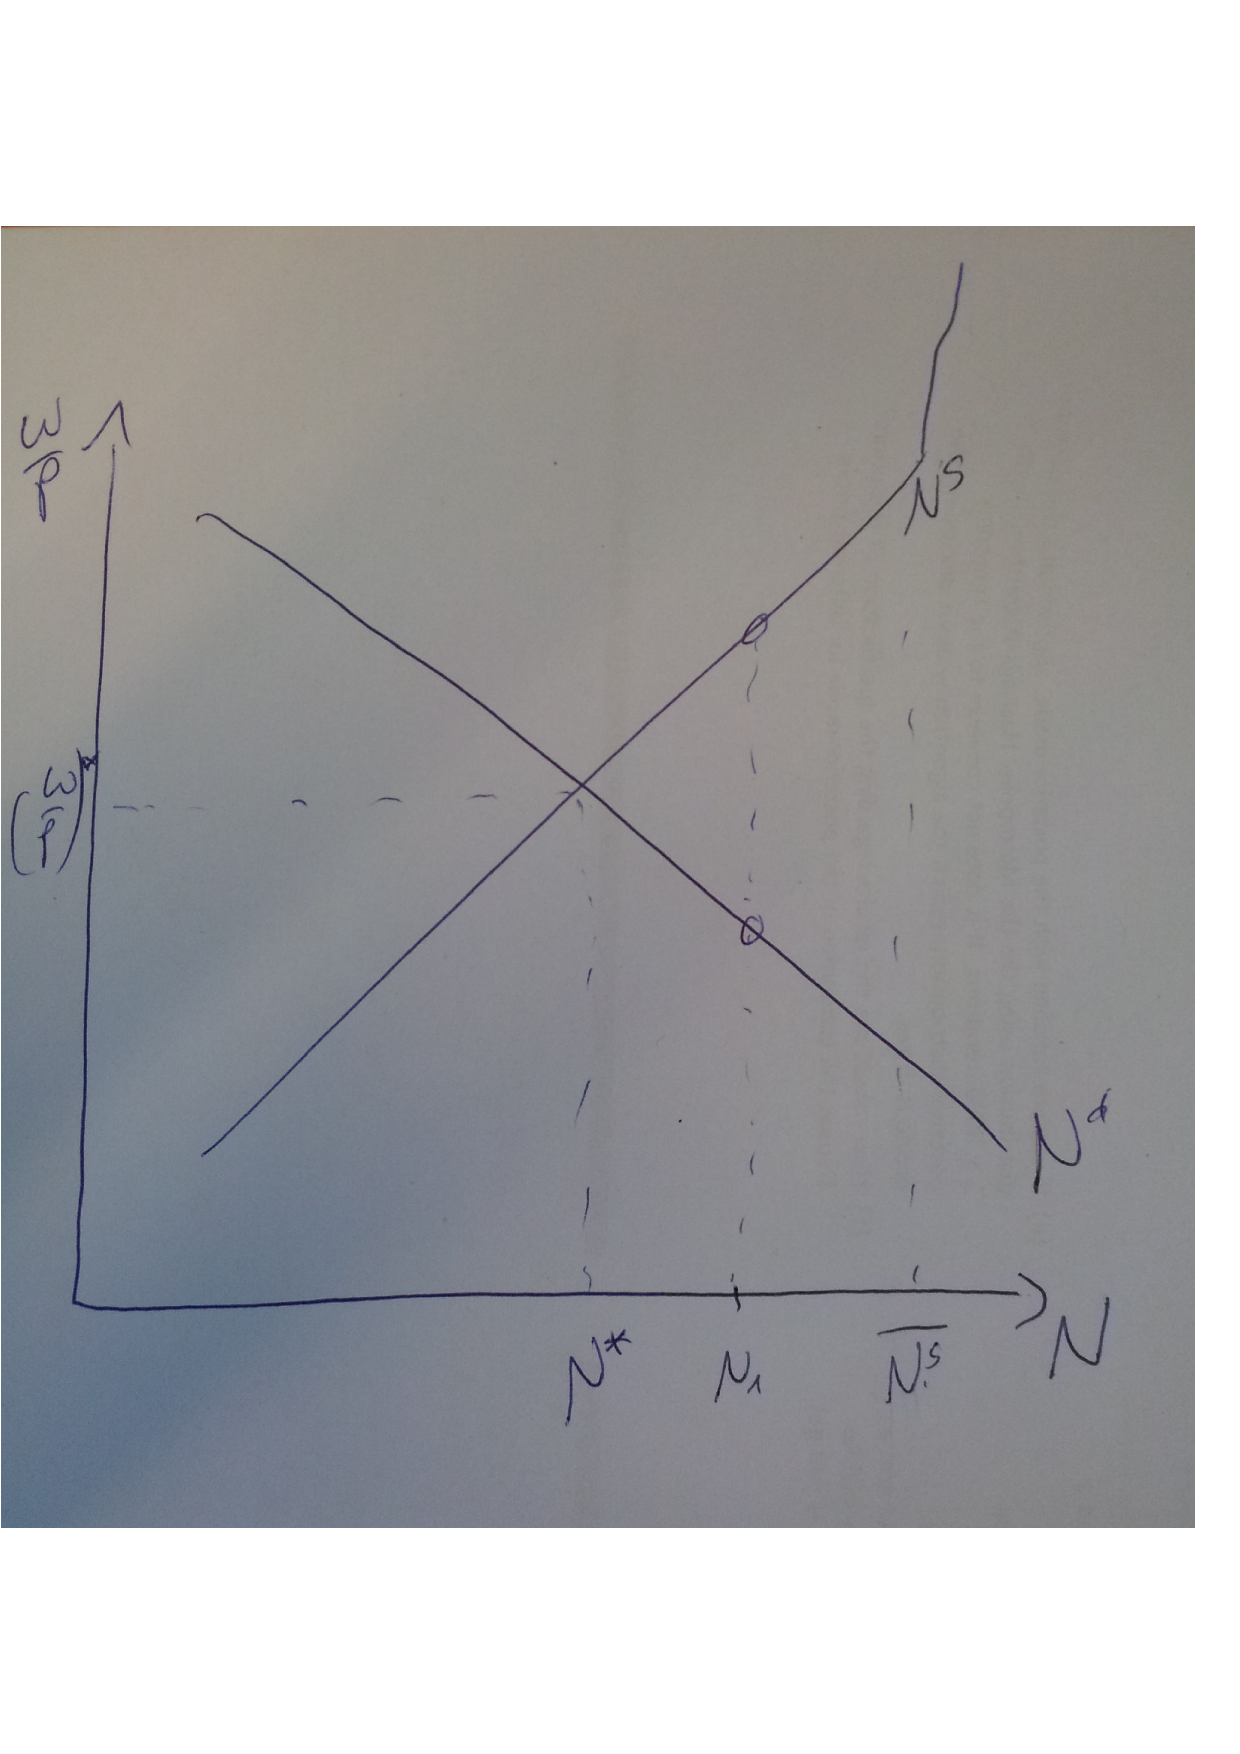
\includegraphics[width=.5\textwidth]{Bilder/Arbeitsmarkt.pdf}\\
%  Vollbesch\"{a}ftigung: Niemand ist unfreiwillig arbeitslos. D.h. z.B. $(N_1-N^*)$ Arbeitnehmer sind freiwillig arbeitslos, da ihnen der gebotene Reallohn zu gering erscheint. Arbeitslosigkeit im klassisch-neoklassischen Modell bezeichnet nur unfreiwillige Arbeitslosigkeit! Anhaltende unfreiwillige Arbeitslosigkeit kann der klassisch-neoklassischen Theorie zufolge NICHT auftreten, da der Lohnmechanismus Angebot und Nachfrage ausgleicht!
%  \item \Tree [.{Kapitalmarkt (Handel von WP)} [.Wertpapierangebot [.{\bf Unternehmen} $I(R)=\frac{\Delta B^s}{P}$ ] ] [.Wertpapiernachfrage [.{\bf Haushalte} $S(R)=\frac{\Delta B^d}{P}$  ]  ] ]\\
%  Unternehmen beachten bei ihrer Planung die Produktionsm\"{o}glichkeiten abh\"{a}ngig von $F(\underbrace{N}_\text{Auf AM bestimmt},\underbrace{K}_\text{Auf KM bestimmt})$. Investitionen = Ver\"{a}nderung des physischen Kapitalbestandes: $I = K-K_0$. Investitionen werden durch Ausgabe von Wertpapieren finanziert, d.h. $p \cdot I(R) = \Delta B^s$ ist Kapitalnachfrage. Die Haushalte bieten dazu ihre Ersparnisse an, d.h. $p \cdot S(R) = \Delta B^d$. Zinssatz passt sich so an, dass $S(R)=I(R)$ gilt. \\
%  Wichtig: $I(R)$ kommt aus der Bedingung f\"{u}r gewinnmaximalen Kapitaleinsatz, $GPK = \frac{\partial F(N,K)}\partial K = R$. Also in jedem Punkt der I-Kurve gilt $GPK = R$, da die I-Kurve alle gewinnmaximalen Kombinationen von Zins und Investitionen abbildet.
%  \item G\"{u}termarkt
%
%  \begin{align*}
%  Y^S(N) = \underbrace{Y^S(W/P)}_\text{G\"{u}terangebot} = \underbrace{C(i)+I(i)}_\text{G\"{u}ternachfrage}
%  \end{align*}
%  Gesetz von Walras: Grundidee:
%  \begin{tabular}{c|c|c}
%    Markt & Unternehmen  & Haushalte \\
%  \hline  Arbeitsmarkt& $N^d$  & $N^S$  \\
%  \hline  Kapitalmarkt& $I$  & $S$  \\
%  \hline  G\"{u}termarkt& $Y^s$  & $C$
%  \end{tabular}
%  Beide Akteure k\"{o}nnen nur zwei Gr\"{o}{\ss}en frei w\"{a}hlen, die dritte ergibt sich automatisch.\\
%  Gesetz von Walras: Die Summe aller \"{U}berschussnachfragen muss gleich null sein.\\
%  Implikationen:
%  \begin{itemize}
%	\item Herrscht auf zwei von drei M\"{a}rkten ein Gleichgewicht, dann ist die \"{U}berschussnachfrage auf dem dritten Markt automatisch null, d.h. der dritte Markt ist ebenso im Gleichgewicht. Bei der makro\"{o}konomischen Analyse gen\"{u}gt es also, das Zustandekommen eines Gleichgewichts auf zwei M\"{a}rkten explizit zu analysieren.
%	\item   Bei positiver Summe der \"{U}berschussnachfrage auf zwei M\"{a}rkten muss ein \"{U}berschussangebot auf dem dritten Markt in entsprechender H\"{o}her vorliegen.
%  \end{itemize}
%
%\item Quantit\"{a}tsgleichung und Quantit\"{a}tstheorie
%\textbf{I) Quantit\"{a}tsgleichung:}\\
%1. Wert des G\"{u}terkaufs = gezahlter Betrag, aufsummieren \"{u}ber alle Transaktionen ergibt $P H = Z$, wobei P: Durchschnittspreis aller gekauften G\"{u}ter, H: gesamte Handelsvolumen, Z: Summe aller gezahlten Betr\"{a}ge\\
%2. $Z=Mv$ wobei M: Bestand an Zahlungsmitteln, $v$: durschnittliche Verwendungsh\"{a}ufigkeit (Umlaufgeschwindigkeit)\\
%1+2: $M v = PH$ dies ist die Quantit\"{a}tsgleichung, eine Identit\"{a}tsgleichung! Problem: in H sind auch Vorleistungen enthalten. F\"{u}r Zusammenhang mit realem Volkseinkommen gilt $Y<H$, d.h. $P_y Y= M v_y$ mit $v_y<v$ die Umlaufgeschwindigkeit im EK-Kreislauf und Y reales Volkseinkommen. $v_y$ ist \"{u}ber Gleichung definiert!\\
%Allg:\\
%\begin{itemize}
%\item KEINE KAUSALEN AUSSAGEN K\"{O}NNEN GETROFFEN WERDEN!
%\item \"{A}ndert sich eine Variable, muss sich auch eine andere \"{a}ndern, welche ist unklar.
%\end{itemize}
%II. Quantit\"{a}tstheorie:\\
%Aussagen \"{u}ber den Zusammenhang zwischen Geldmenge und Preisniveau werden abgeleitet: $P=f(M)$
%\begin{itemize}
%\item Ausgestaltung von f folgt aus der Quantit\"{a}tsgleichung: $P = \underbrace{\frac{v}{Y}}_\text{konstant bzw. exogen} M$
%\item Es werden Verhaltensannahmen getroffen:
%\begin{itemize}
%\item Zahlungsmittel werden gleich oft verwendet, v ist weitgehend konstant und nur von langsam \"{a}ndernden Zahlungsgewohnheiten (exogen) beeinflussbar
%\item Realeinkommen ist realwirtschaftliche bestimmt
%\end{itemize}
%\end{itemize}
%Dann l\"{a}sst sich schlie{\ss}en:\\
%\enquote{Ver\"{a}nderungen des Preisniveaus werden (in proportionaler Weise) von Ver\"{a}nderungen der Geldmenge bestimmt} --> Kausalit\"{a}t!
%
%\item (Neo-)klassische Gesamtmodell
%\begin{align*}
%\text{Realer Sektor} = \begin{cases}
%\text{(1) Gleichgewicht auf dem Arbeitsmarkt: } N^d(W/P) = N^s(W/P) &\Rightarrow N^*;(W/P)^*\\
%\text{(2) Produktionsfunktion: } Y=f(N) & \Rightarrow Y^*\\
%\text{(3) Kapitalmarkt: } S(i)=I(i) & \Rightarrow i^*\\
%\end{cases}
%\end{align*}
%
%\begin{align*}
%\text{Monet\"{a}rer Sektor} = \begin{cases}
%\text{(4) Quantit\"{a}tstheorie: } P=\frac{Mv}{Y} &\Rightarrow P^*\\
%\text{(5) Identi\"{a}t: } W=\frac{W}{P}P & \Rightarrow W^*
%\end{cases}
%\end{align*}
%Realer Sektor determiniert alle realen Gr\"{o}{\ss}en, w\"{a}hrend monet\"{a}rer Sektor nur nominale Gr\"{o}{\ss}en determiniert --> \textbf{DICHOTOMIE}\\
%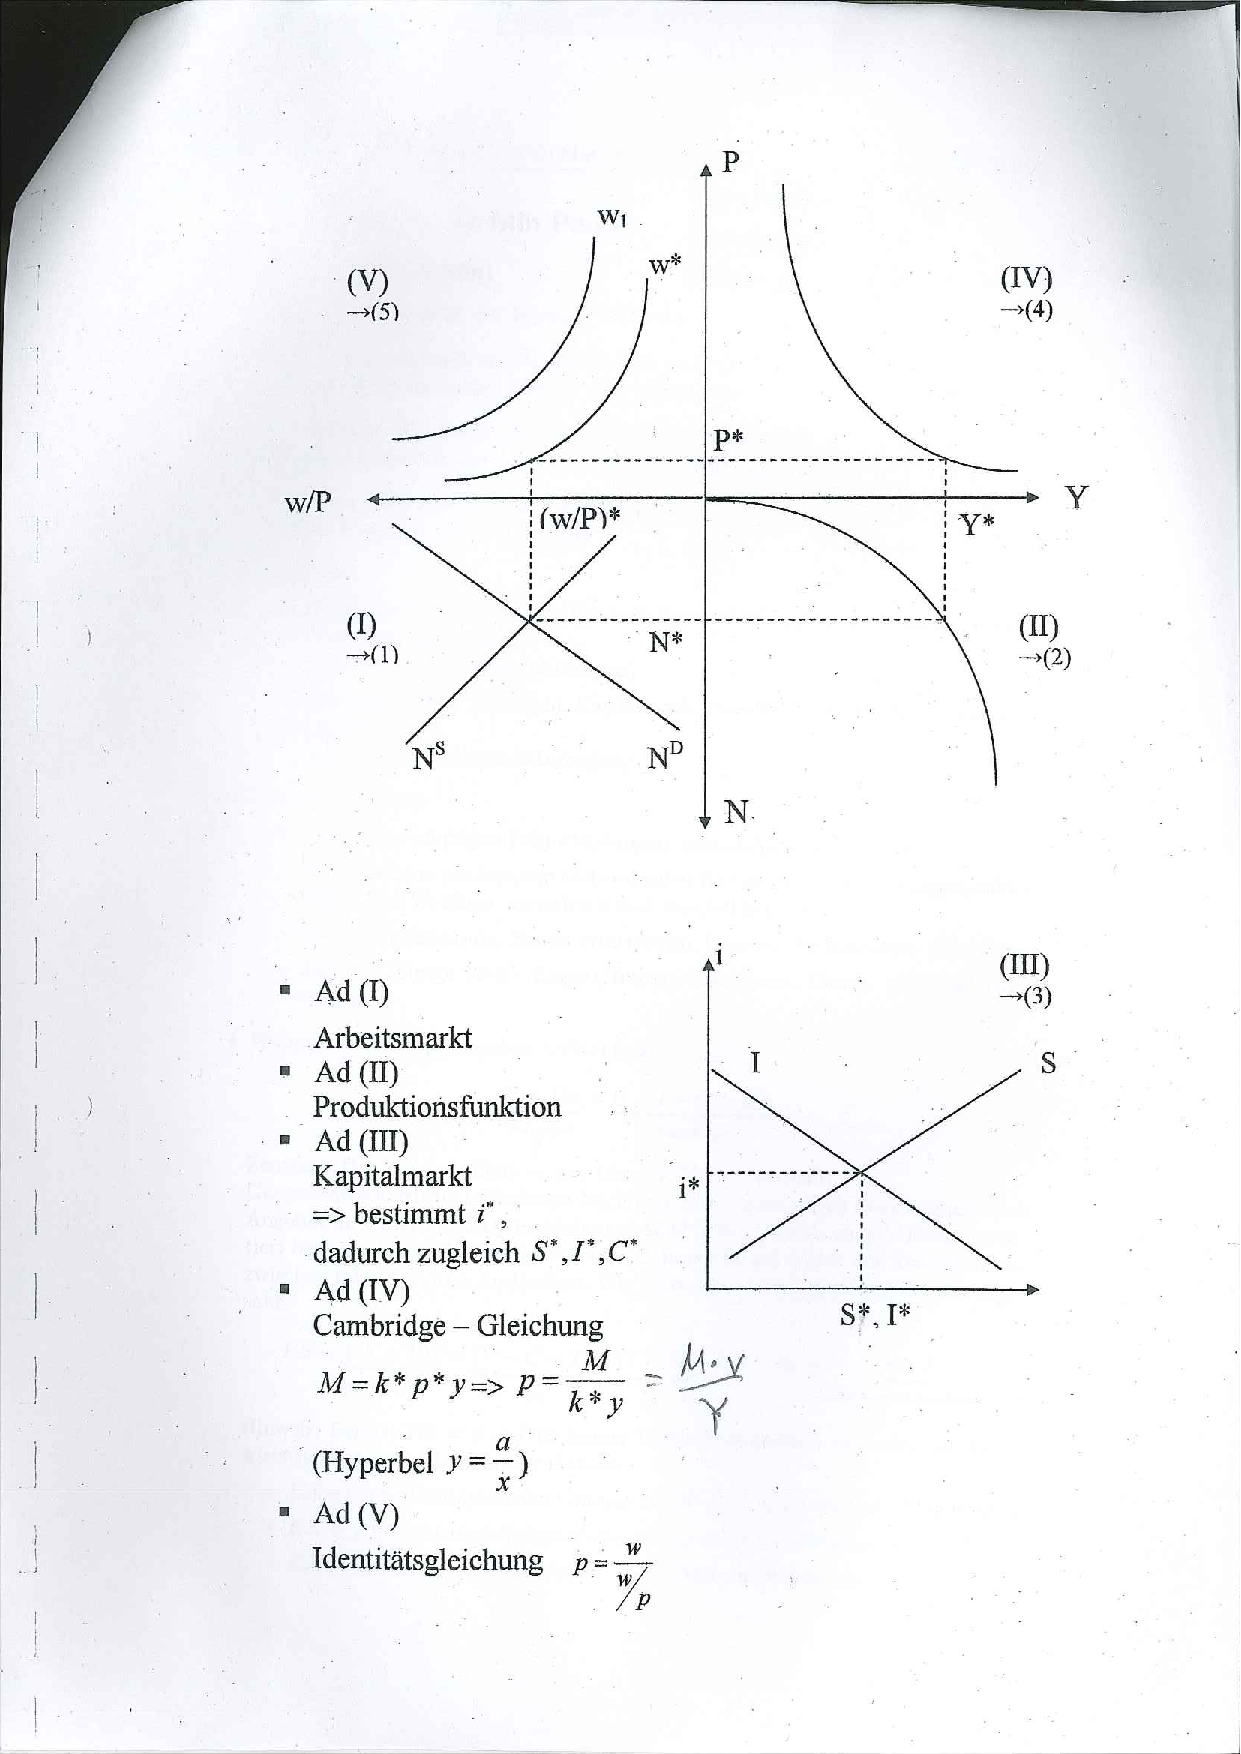
\includegraphics[width=0.9\textwidth]{Bilder/NeoklassikGesamt.pdf}\\
%\textbf{Wann verschieben sich die Kurven?}
%\begin{itemize}
%  \item Produktionsfunktion: Kapital oder Technologieniveau\"{a}nderungen (schiebt sich nach au{\ss}en)
%  \item Geldnachfrage: Kapital oder Technologieniveau\"{a}nderungen (schiebt sich nach au{\ss}en) (analog zur Produktionsfunktion)
%  \item Geldnachfrage: Exogene Einflussfaktoren auf Arbeitsangebot
%  \item Cambridge-Gleichung: Bei Steigerung von Umlaufgeschwindigkeit oder Geldmenge schiebt sich Kurve nach au{\ss}en
%  \item Lohnkurve: Schiebt sich nach au{\ss}en bei Nominallohnsteigerungen oder Preissteigerungen
%  \item I und S \"{a}ndern sich bei Pr\"{a}ferenz\"{a}nderungen
%\end{itemize}
%\item Wirtschaftspolitik in der Neoklassik:\\
%Modell erweitern:
%\begin{align*}
%Y &= C+G+I &\text{ G\"{u}termarkt}\\
%Y &= C-T+S &\text{ Budgetrestriktion}\\
%S &= I + D	&\text{Kapitalmarkt}\\
%D &= G-T &\text{Staatsbudget, D ist Neuverschuldung}
%\end{align*}
%\begin{enumerate}[(i)]
%\item Kreditfinanzierte Staatsausgabenerh\"{o}hung: T=0, D=G, Staat wird auf Kreditmarkt aktiv, d.h.
%\begin{align*}
%S=I+D =I+G
%\end{align*}
%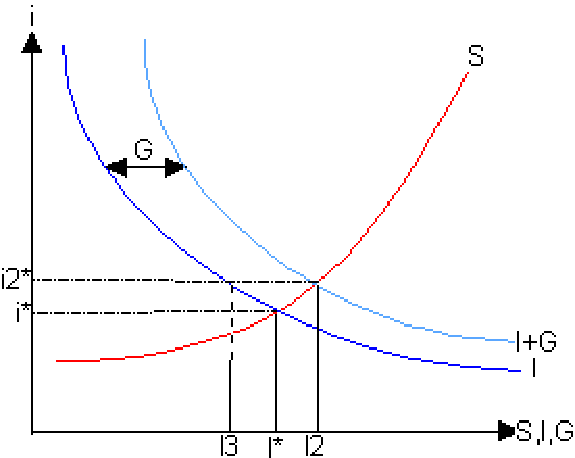
\includegraphics[width=0.5\textwidth]{Bilder/CrowdingOut.pdf}\\
%2 Effekte:\\
%1. $i\uparrow \rightarrow I \downarrow$ Investitions-Crowding-Out\\
%2. $i\uparrow \rightarrow S \uparrow \rightarrow C \downarrow$ Konsum-Crowding-Out\\
%In Summe ergibt das vollst\"{a}ndiges Crowding-Out, denn Nachfrage muss insgesamt immer noch gleich Angebot sein $Y^d=Y^s$. $Y^s$ wird aber \"{u}ber den Arbeitsmarkt mithilfe der Produktionsfunktion bestimmt!
%
%\item Steuerfinanzierte Staatsausgabenerh\"{o}hung: $T=G,D=0$
%\begin{align*}
%Y-T = C+S,\qquad T\uparrow &\rightarrow C \downarrow\\
%& \rightarrow S \downarrow \rightarrow i \uparrow \rightarrow I \downarrow
%\end{align*}
%Auch hier vollst\"{a}ndiges Crowding-Out, nur Komposition zwischen C und S \"{a}ndert sich aufgrund ver\"{a}ndertem Zins.
%\item Geldpolitik: Erh\"{o}hung des Geldangebots: $M\uparrow$
%\begin{align*}
%M = \frac{Y}{v} P\\
%M \uparrow \rightarrow P \uparrow
%\end{align*}
%Cambridge-Effekt: H\"{o}here Geldmenge f\"{u}hrt zu h\"{o}herer G\"{u}ternachfrage $(Y^d>Y^s)$, aber $Y^s$ konstant. D.h. Preis muss steigen $(P\uparrow)$, aber dann sinkt auch die Nachfrage wieder bis $Y^d=Y^s$ gilt. Reale Geldmenge $\frac{M}{P}$ bleibt konstant!
%\end{enumerate}
%
%Merke:\\
%(1) Fiskalpolitik nicht erforderlich, da das (neo-)klassische Modell von sich aus das Vollbesch\"{a}ftigungsgleichgewicht erreicht! Fiskalpolitik f\"{u}hrt zu vollst\"{a}ndigem Crowding-Out, da das Arbeitsangebot allein vom Reallohn abh\"{a}ngt und somit die Produktion und Einkommen unver\"{a}ndert bleiben. Nur die Verteilung und der Zins \"{a}ndern sich.\\
%(2) Geldpolitik beeinflusst nur das Preisniveau!
%\item Rechenaufgabe:\\
%\begin{enumerate}[(1)]
%\item $N^d = 4 \left(\frac{W}{P}\right)^{-2}$
%\item $(W/P)^*=2,N^*=1,Y^*=4,Lohnsumme=N^* W^* = 2, Gewinn = 2$
%\end{enumerate}
%\item Verst\"{a}ndnisfragen:
%\begin{enumerate}[1.]
%\item wahr, BR gilt immer f\"{u}r alle Kombis
%\item falsch, da Arbeitsnachfrage steigt f\"{u}r jeden Lohn
%\item wahr
%\item wahr
%\item wahr
%\item wahr
%\item falsch
%\item wahr
%\item falsch
%\item wahr
%\item falsch
%\item falsch
%\item falsch
%\item falsch
%\item wahr
%\item falsch
%\item falsch
%\item falsch
%\item falsch
%\item falsch
%\item wahr
%\item falsch
%\item falsch
%\item wahr
%\item falsch
%\item wahr
%\item falsch
%\item wahr
%\item wahr
%\item falsch
%\item falsch
%\item falsch
%\item falsch
%\item falsch
%\item wahr
%\item falsch
%\item wahr
%\item wahr
%\item falsch
%\item falsch
%\item wahr
%\end{enumerate}
%\end{enumerate}
%
%



\section{G\"{u}termarkt und IS-Kurve}
\subsection{Sparfunktion, marginale Neigungen und Multiplikatoren}
\begin{enumerate}[(a)]
%\item Fundamentale Unterschiede zur neoklassischen Theorie:
%\begin{itemize}
%\item Gleichgewichtsbegriff
%\begin{itemize}
%  \item Klassik-GG: Marktr\"{a}umung
%  \item Keynes-GG: Keine inneren Anreize zum Abweichen
%\end{itemize}
%\item Lohn- und Preisrigidit\"{a}ten\\
%Hindernisse erschweren insbesondere Lohn- und Preissenkungen:
%    \begin{itemize}
%      \item Vermachtung (Marktkonzentration)
%      \item Psychologische Ursachen
%      \item Institutionelle Ursachen (Vertragslaufzeiten)
%    \end{itemize}
%    Preise nehmen nicht zwangsl\"{a}ufig Marktr\"{a}umungswerte an, d.h. umgesetzte Mengen bestimmt durch Minimumsregeln $Y=min(Y^s,Y^d)$, k\"{u}rzere Seite gewinnt.
%\item Effektive Nachfrage\\
%    Definition: Wert des Volkseinkommens bei dem ein GG auf dem gesamtwirtschaftlichem G\"{u}termarkt herrscht $Y^d=Y^s$. F\"{u}r Konsum ist tats\"{a}chliches verf\"{u}gbares Einkommen relevant.\\
%    Schematisch:\\
%    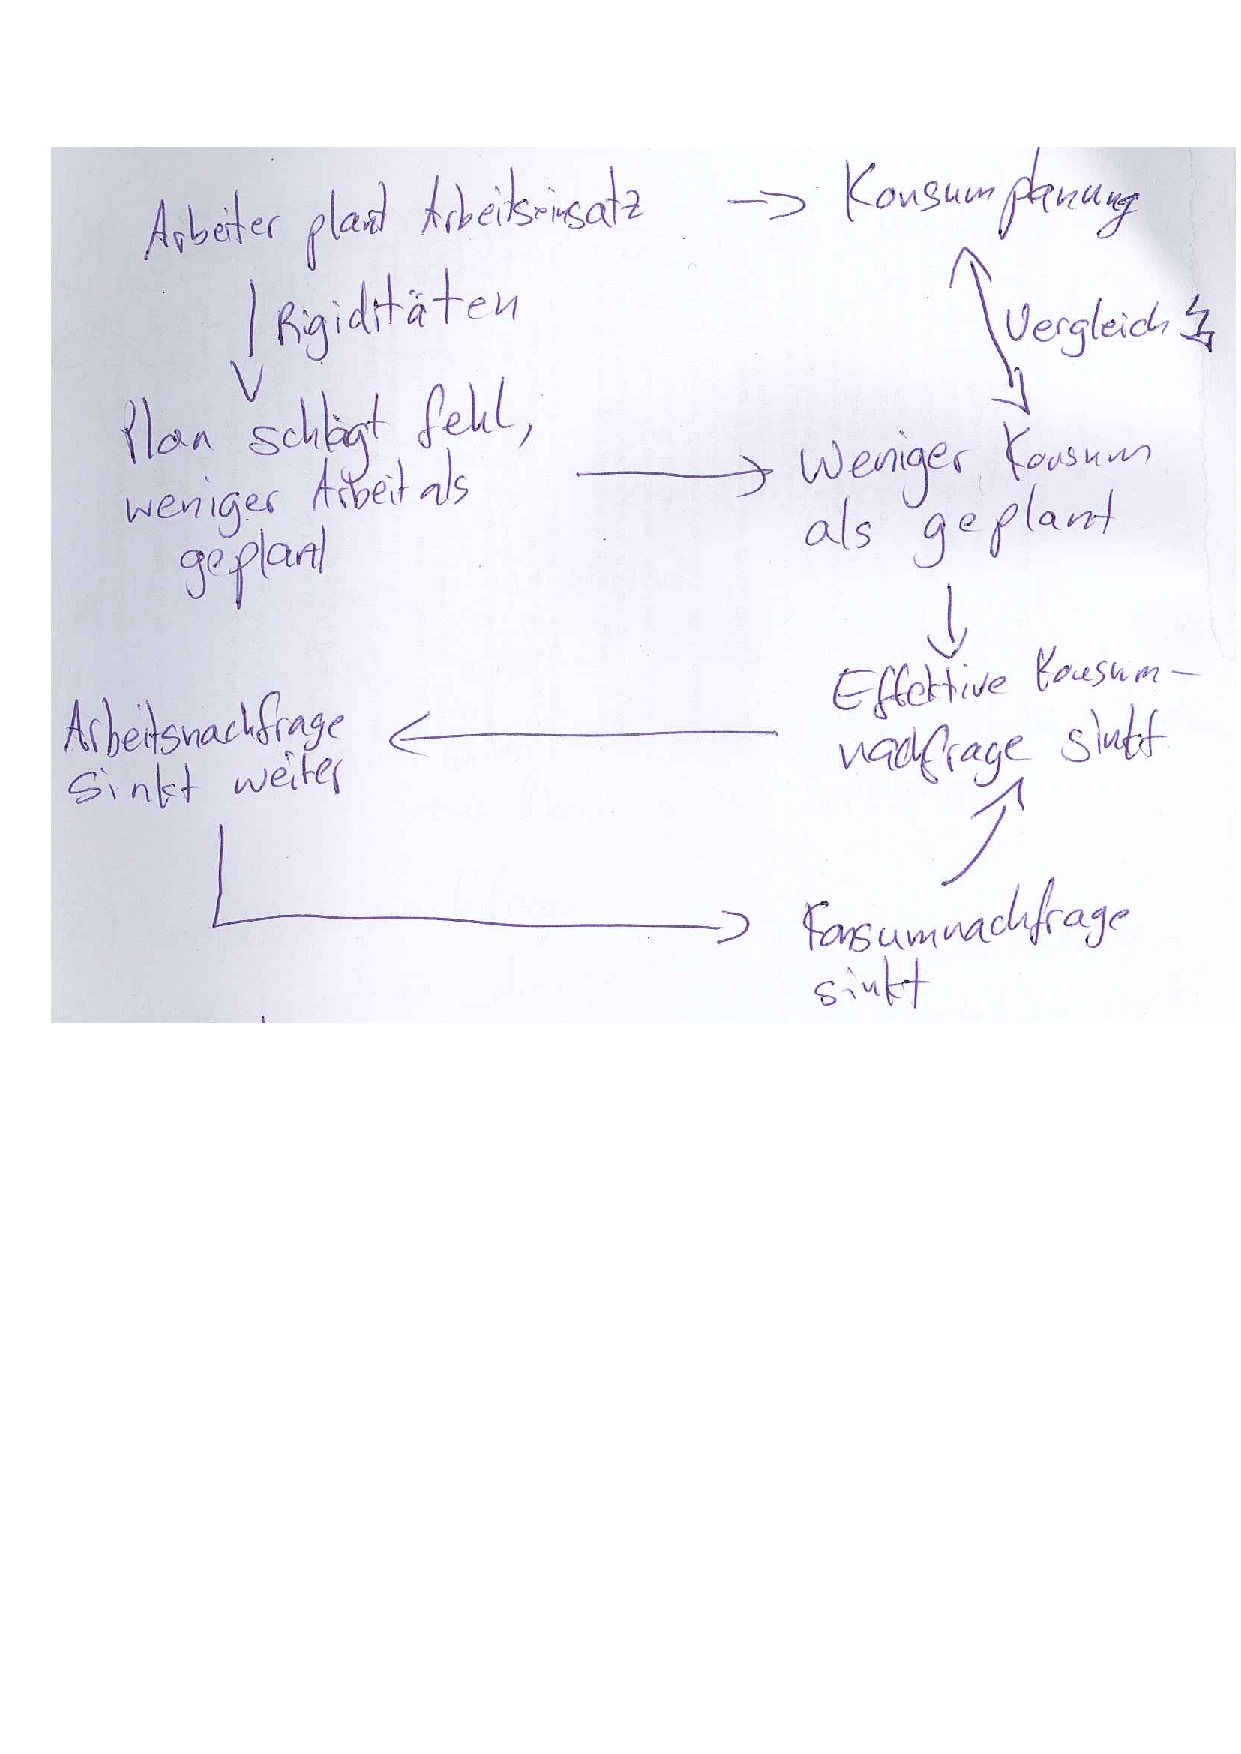
\includegraphics[width=\textwidth]{Bilder/Effektive_Nachfrage.pdf}
%\item Rationierung\\
%Unternehmen sind auf G\"{u}termarkt rationiert (effektive G\"{u}ternachfrage)\\
%Haushalte sind auf Arbeitsmarkt rationiert (effektive Arbeitsnachfrage)
%\end{itemize}
\item Gleichungen (basierend auf Keynes Annahmen)
\begin{enumerate}[(1)]
  \item Konsumnachfrage (linear, Verhaltensgleichung): $C=\underbrace{c_{0}}_\text{exogen} + c_1 \underbrace{Y}_\text{endogen}$\\
  Konsum heute h\"{a}ngt vom verf\"{u}gbaren Einkommen \emph{heute} ab und nicht von Plangr\"{o}{\ss}en! $c_{0}$ ist autonomer Konsum und $c_1 = \partial C / \partial Y$ die sogenannte marginale Konsumneigung.\\
%  Unterschiede zur Neoklassik:
%  \begin{itemize}
%    \item Kein intertemporaler Ausgleich (Konsum nicht von i abh\"{a}ngig)
%    \item Keine simultane Planung von EK und Konsum bzw. Planung ist irrelevant
%  \end{itemize}
  \item Investitionsnachfrage (Verhaltensgleichung, hier: funktional Zinsabh\"{a}ngig, ABER i ist exogen, also $I=\overline{I}$!)\\
  Idee: Investiere solange bis die Grenzleistungsf\"{a}higkeit einer zus\"{a}tzlichen Investition gr\"{o}{\ss}er als der Zins ist. Grenzleistungsf\"{a}higkeit des Kapitals nimmt mit einer zus\"{a}tzlichen Einheit Kapital ab: $I=I(\overset{-}{r})=\underbrace{I_{0}}_\text{exogen} - b \underbrace{ri}_\text{hier exogen,da r gegeben sp\"{a}ter endogen}$.\\
%  Funktional \"{a}hnlich der neoklassischen Investitionsfunktion, aber Einsch\"{a}tzung der Grenzleistungsf\"{a}higkeit ist stark psychologisch bestimmt (interner Zinssatz einer Investition)
  \item Aggregierte Nachfrage (Identit\"{a}tsgleichung), effektive Nachfrage, $Y^d = C+I$, alles endogen
  \item Gleichgewichtsgleichung, Im Gleichgewicht gilt Nachfrage = Angebot $(Y^s=Y^d)$, insbesondere bei Keynes antizipierte Nachfrage = tats\"{a}chliche Nachfrage
  \item Unternehmen passen Produktion an erwartete Nachfrage an (Verhaltensgleichung):
  \begin{itemize}
    \item Produktion $Y^S$ h\"{a}ngt ab von der Nachfrage $Y^d$
    \item Nachfrage h\"{a}ngt ab vom Einkommen
    \item Einkommen wird durch Produktion bestimmt
    \item Y ist also Einkommen, Nachfrage und Produktion im Gleichgewicht!
    \item ENDOGENER PROZESS
  \end{itemize}
  $(3)+(4)+(5) \Rightarrow Y^s=Y=Y^d$, Y ist endogen!
\end{enumerate}

\item \textbf{Sparfunktion:}
\begin{itemize}
\item \textbf{\emph{Analytische Herleitung:}}
    \begin{align*}
      S=Y-C=Y-c_{0}-c_1 Y = -c_{0}+(1-c_1) Y\\
      \Leftrightarrow S = -c_{0} + \underbrace{(1-c_1)}_{\equiv s} Y = -c_{0} + s Y
    \end{align*}
    Marginale Konsumneigung: $\frac{\partial C}{\partial Y} = c_1$ und marginale Sparneigung: $\frac{\partial S}{\partial Y} = 1-c_1\equiv s$
\item \textbf{\emph{Grafische Herleitung}}
\begin{center}
  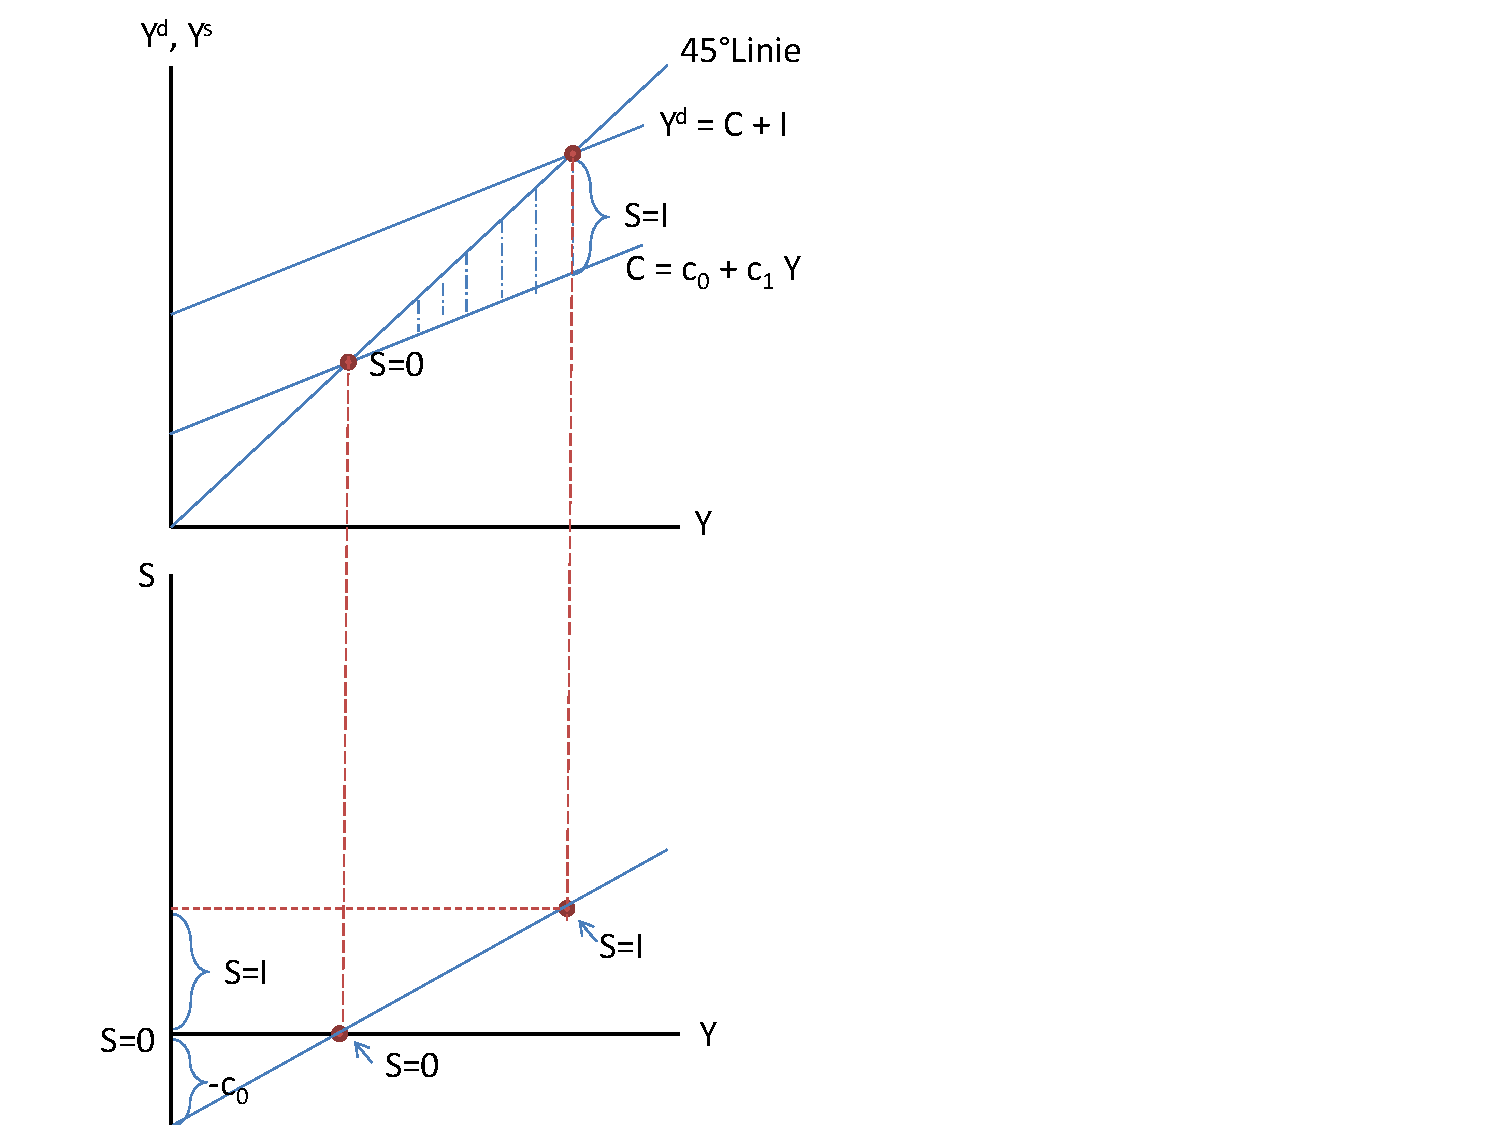
\includegraphics[width=.6\textwidth]{Bilder/sparfunktion.pdf}\\
\end{center}
\end{itemize}

\item
\textbf{Bestimmung des gleichgewichtigen Einkommens}
\begin{enumerate}[(i)]
  \item Keynesianische Kreuz
  \begin{align*}
    Y=C+I=c_{0}+c_1 Y + I_{0} -b r\\
    Y= \frac{1}{1-c_1} (c_{0} + I_{0} - b r)
  \end{align*}
  \begin{center}
  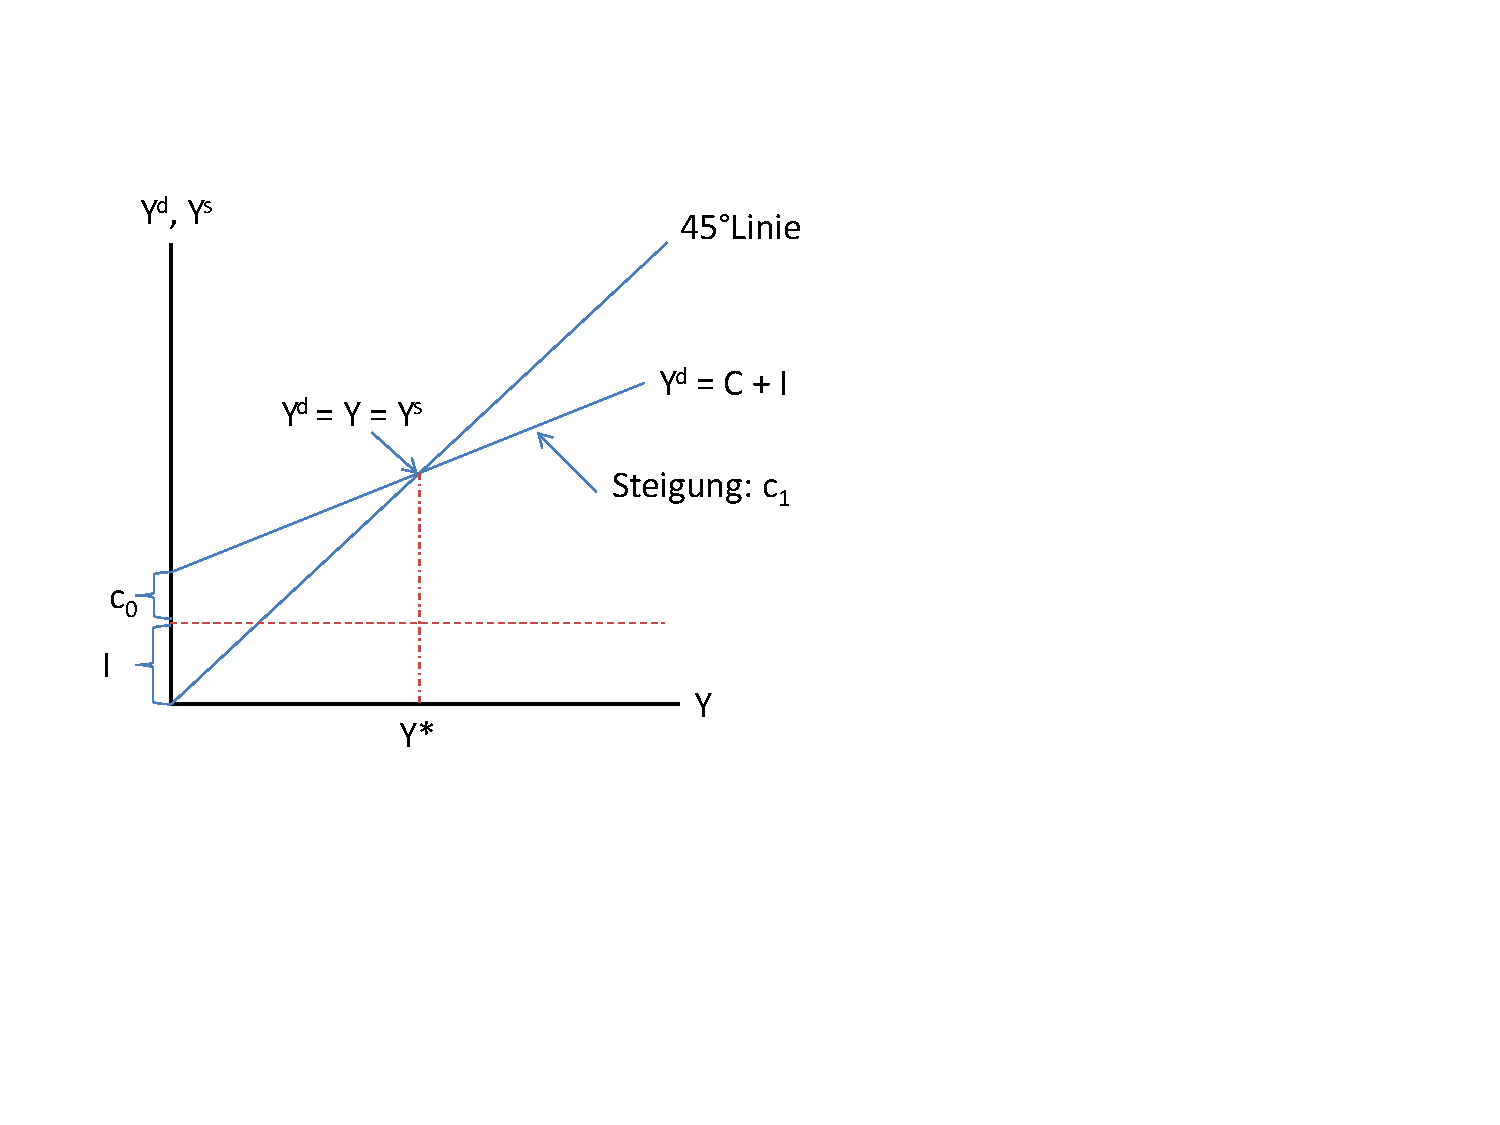
\includegraphics[width=.5\textwidth]{Bilder/ISGG1.pdf}
  \end{center}
  \item Sparfunktion
  \begin{align*}
    S=I \Leftrightarrow -c_{0} + (1-c_1)Y = I_{0} -b r\\
    Y= \frac{1}{1-c_1} (c_{0} + I_{0} - b r)
  \end{align*}
    \begin{center}
  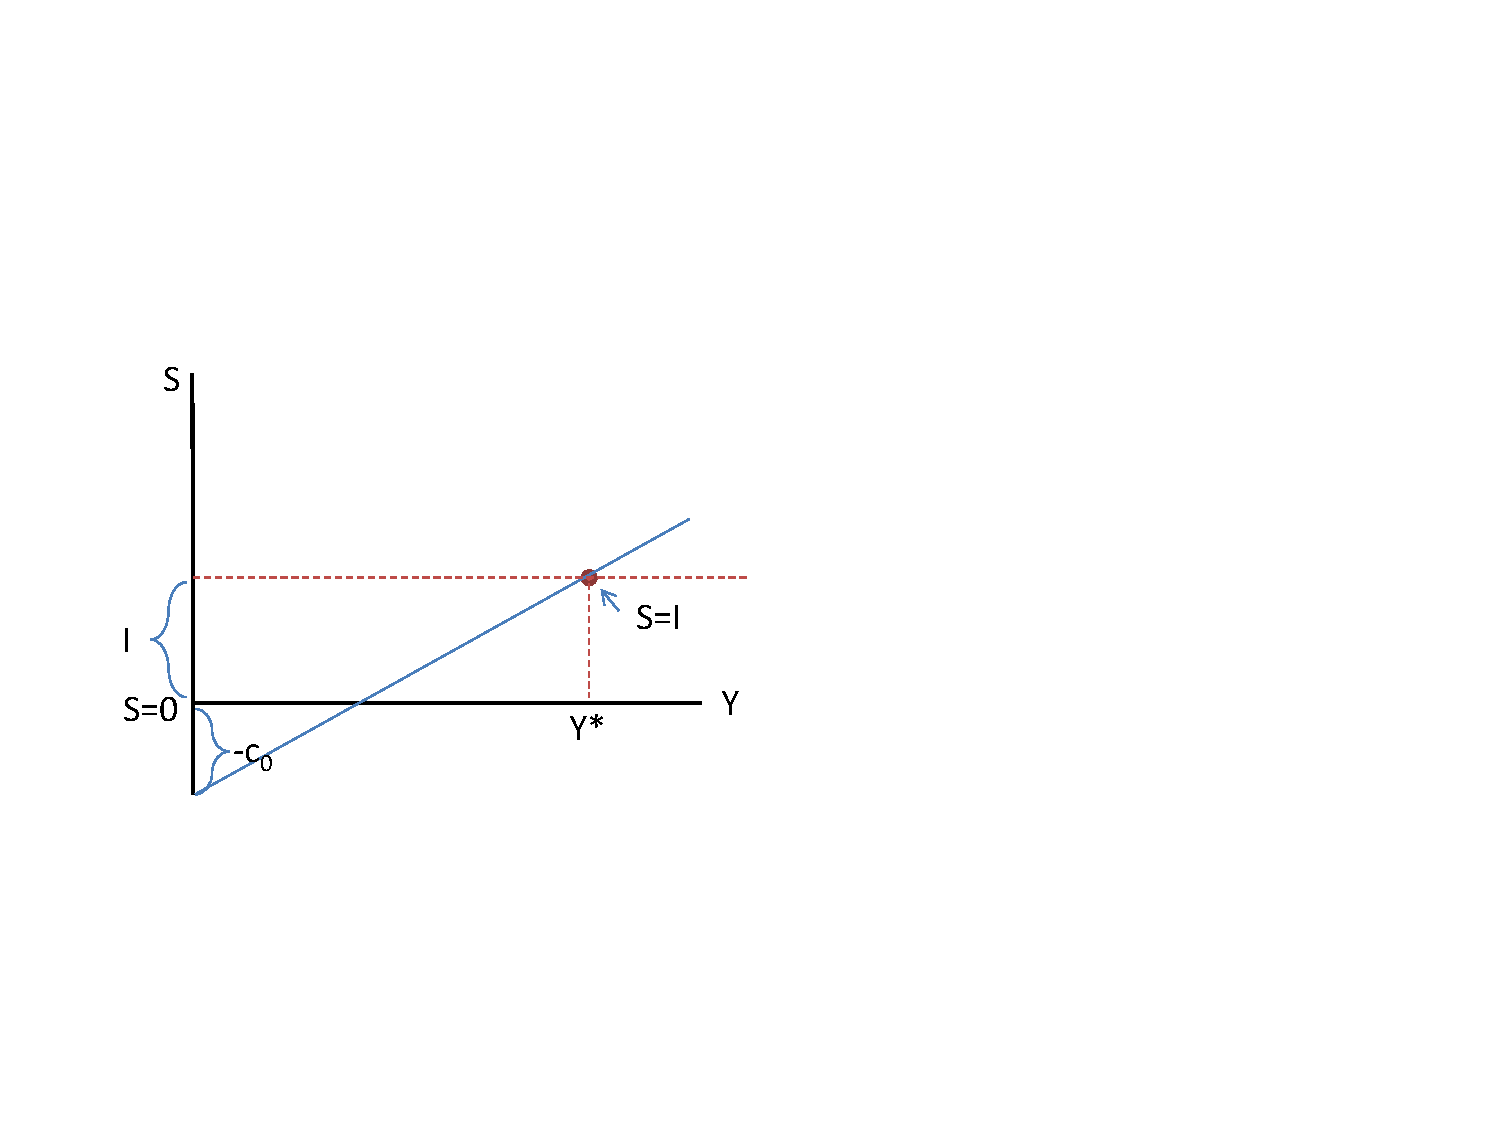
\includegraphics[width=.5\textwidth]{Bilder/ISGG2.pdf}
  \end{center}
\end{enumerate}
Sinnvolles Gleichgewicht existiert nur , wenn $0<c_1<1$, denn sonst ist $Y^* <0$.\\
%\textbf{Vergleich zur Neoklassik:}\\Hier wird das GG \"{u}ber den Arbeitsmarkt und Produktionsfunktion bestimmt! Say: Jedes Angebot schafft sich seine Nachfrage vs. Keynes: Effektive Nachfrage

\item
\begin{enumerate}[(i)]
  \item Erh\"{o}hung von $c_{0}: \frac{\partial Y^*}{\partial c_{0}}=\frac{1}{1-c_1}>1$
  \begin{itemize}
    \item Zunahme in $Y^*$ ist gr\"{o}{\ss}er als die urspr\"{u}ngliche Mehrnachfrage in $c_{0}$
    \item Multiplikatorprozess!
  \end{itemize}
  \item Erh\"{o}hung von $r: \frac{\partial Y^*}{\partial r}=-b\frac{1}{1-c_1}<0$
  \begin{itemize}
    \item Sinkende Investitionen f\"{u}hren zu sinkendem gleichgewichtigen Einkommen (sp\"{a}ter nennen wir das die IS-Kurve!)
  \end{itemize}
\end{enumerate}
\textbf{Der Multiplikatorprozess:}
\begin{center}
  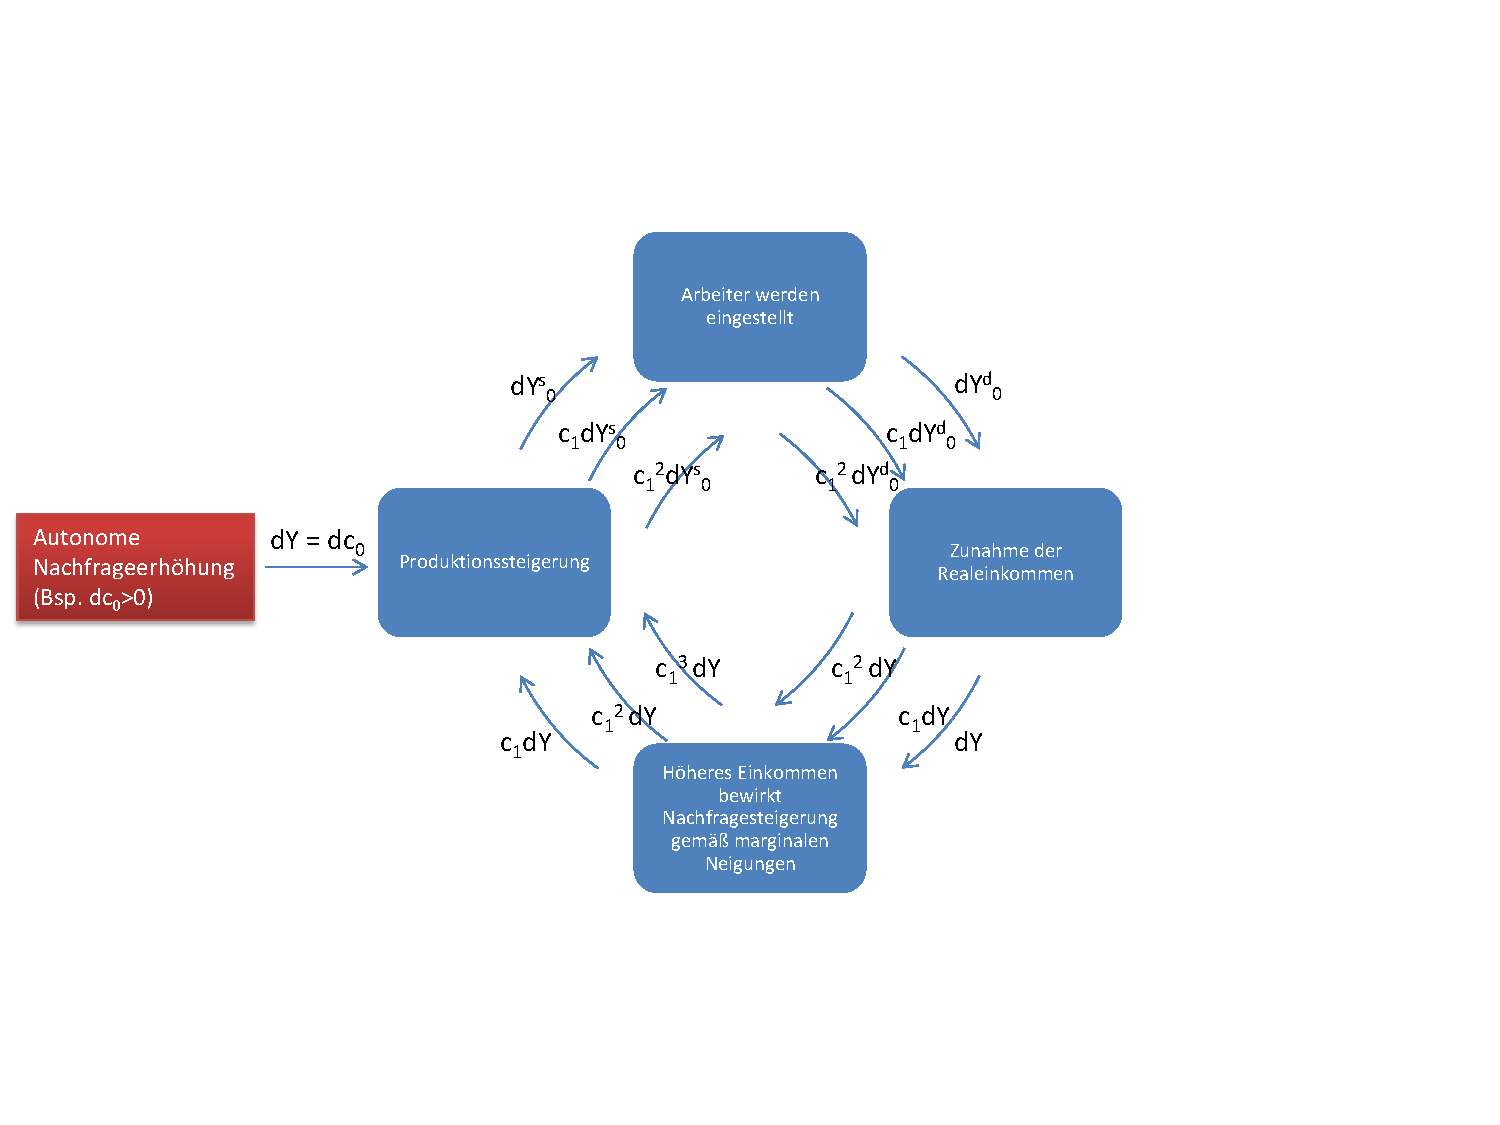
\includegraphics[width=\textwidth]{Bilder/multiplikator.pdf}
\end{center}
\begin{align*}
  d Y^* &= d c_{0} + c_1 d c_{0} + c_1^2 d c_{0} + \dots = d c_{0} \cdot \overbrace{\underbrace{(1 + c_1 + c_1^2+ \dots)}}_{=\frac{1}{1-c_1}, \text{falls } 0<c_1<1}^\text{Unendlichte geometrische Reihe}= \frac{1}{1-c_1}dc_{0}, \\\text{ denn:}&\\
  d Y^* - c_1 d Y^* &= d c_{0}(1 + c_1 + c_1^2+ \dots) - c_1 d c_{0}(1 + c_1 + c_1^2+ \dots) \\
  &= d c_{0} + d c_{0}(c_1 + c_1^2+ \dots) - d c_{0}(c_1 + c_1^2+ \dots) \\
  &= d c_{0}\\
  \Leftrightarrow d Y^* &= \frac{d c_{0}}{1-c_1}
\end{align*}
\begin{center}
  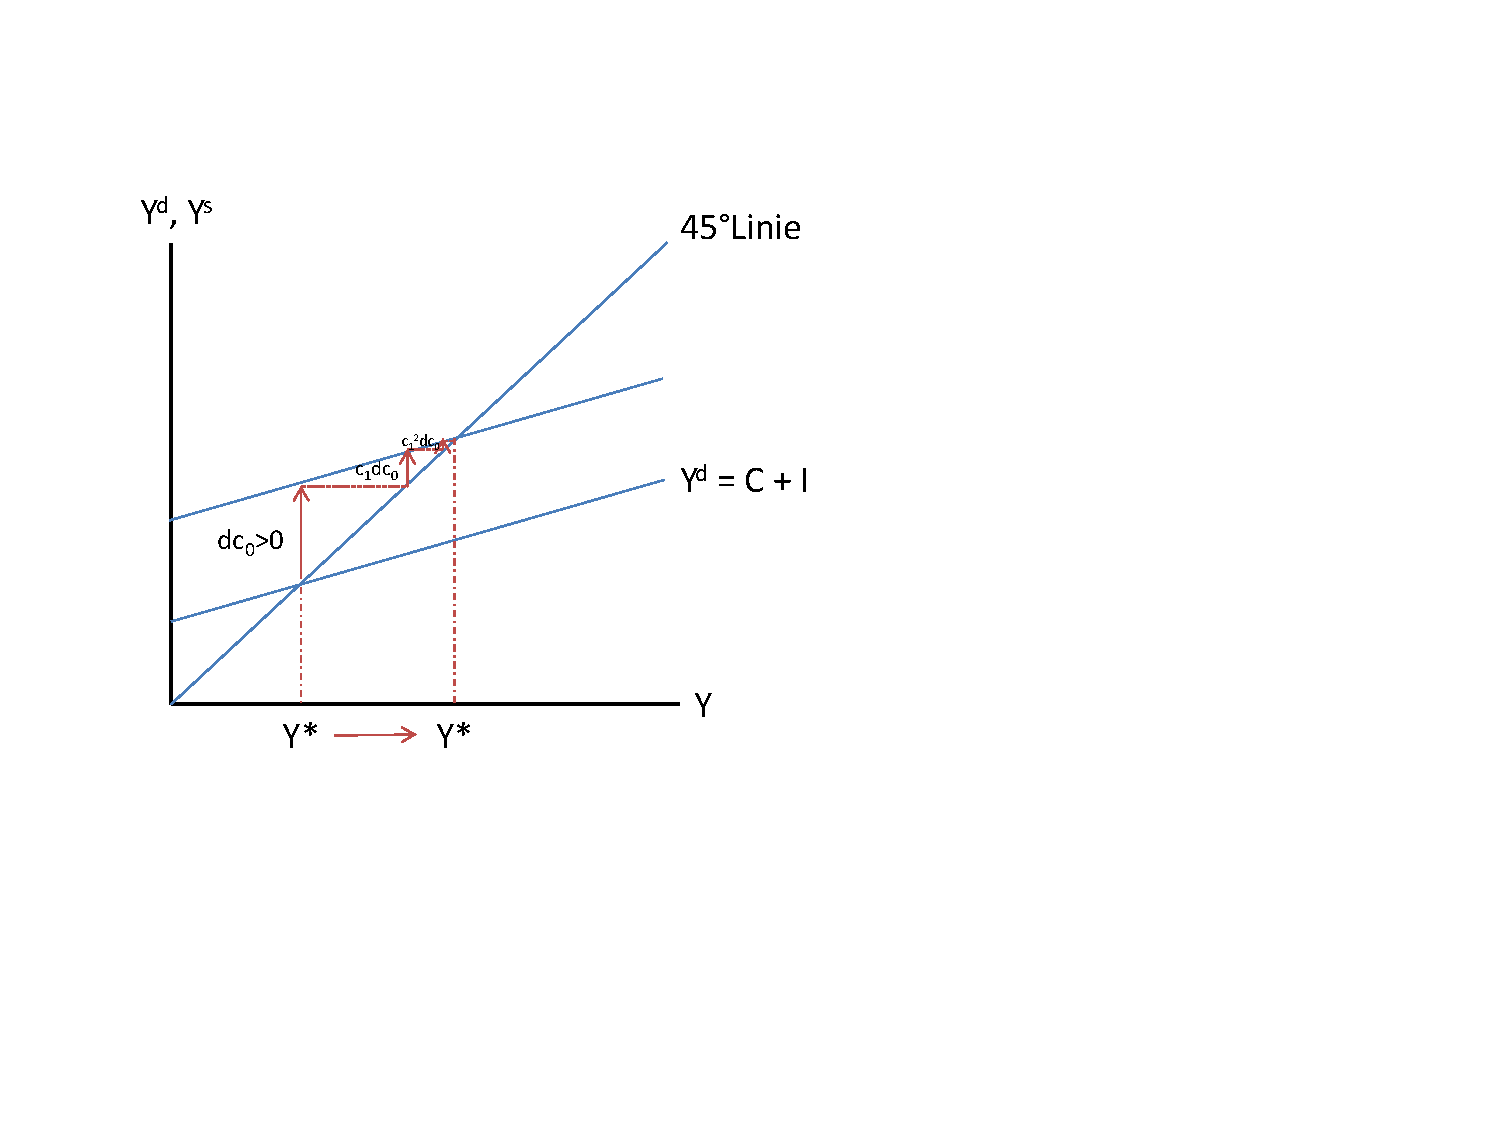
\includegraphics[width=0.5\textwidth]{Bilder/multiplikatorgrafisch.pdf}
\end{center}
\item \begin{align*}
C = c_0 + c_1(Y-T)\\
      S = S^{pr} + S^{St} = (Y-T-C) + (T-G) = \overline{I}\\
      Y = \frac{1}{1-c}(c_0 + \overline{I} + G - c_1 T)
    \end{align*}
\item Sparparadox: $S = S^{pr} + S^{St} = (Y-T-C) + (T-G) = overline{I}$. (i) Aus Staatssicht: Da I konstant ist, gilt, falls die Regierung spart, d.h. $S^{St} \uparrow$, muss $S^{Pr}$ sinken, da die Gesamtersparnis sich nicht ver\"{a}ndern kann. (ii) Haushaltssicht: Wenn HH mehr sparen wollen, d.h. weniger konsumieren, sinkt die gleichgewichtige Produktion und Einkommen im selben Ma{\ss}e $Y^* \downarrow$. Im Endeffekt bleibt die private Ersparnis unver\"{a}ndert. Die Leute m\"{o}chten zwar mehr sparen, aber das Einkommen (und damit die Produktion) muss gerade so stark zur\"{u}ckgehen, dass die Ersparnis unver\"{a}ndert bleibt. Dieses Ph\"{a}nomen wird als Sparparadox bezeichnet.
\begin{enumerate}[(i)]
  \item $dG>0$, d.h.
  \begin{align*}
    dY = \frac{1}{1-c_1} dG \Leftrightarrow (1-c_1)dY=dG\\
    dC = c_1 dY\\
    \Rightarrow dY-c_1 dY = dG \Leftrightarrow dY-dC = dG\\
    \Rightarrow dS = dY-dC-dG = dG-dG = 0
  \end{align*}
  \item $dG=dT$, d.h.
  \begin{align*}
    dY = \frac{1}{1-c_1} (dG -c_1 dT) = \frac{1}{1-c_1}(dG -c_1 dG) = \frac{1-c_1}{1-c_1}dG = dG\\
    \Rightarrow dS = dY-dT - dC +dT -dG = dG-dG = 0
  \end{align*}
    \item $dc_1<0$, d.h.
  \begin{align*}
    dY - c_1 dY -dc_1Y =dc_0 +d\overline{I} +dG - c_1dT -dc_1T
    \Leftrightarrow (1-c_1)dY = dc_1(Y-T)\\
    dC = dc_0 + dc_1(Y-T) +c_1(dY-dT) = dc_1(Y-T) + c_1 dY = (1-c_1)dY + c_1dY = dY\\
    \Rightarrow dY-c_1 dY = dG \Leftrightarrow dY-dC = dG\\
    \Rightarrow dS = dY-dC = 0
  \end{align*}
\end{enumerate}
\end{enumerate}

\subsection{IS-Kurve}
\begin{enumerate}[(a)]
\item \textbf{IS-Kurve Analytisch:}
\begin{itemize}
\item Berechnung der Sparfunktion:
\begin{align*}
  S &= S^{Pr} + S^{St} = (Y-C-T) + (T-G) = Y-c_{0} -c_1\underbrace{(Y-T_{0} - t Y)}_{\equiv Y^v} - G_{0}\\
  \Leftrightarrow S&= -G_{0} - C_{0} - c_1 T_{0} + (1-c_1(1-t))Y
\end{align*}
\item $I(r)=S(Y):$
\begin{align*}
  I_{0} - b r &= -G_{0} - c_{0} - c_1 T_{0} + (1-c_1(1-t))Y\\
  \Leftrightarrow Y &= \frac{1}{1-c_1(1-t)}(c_{0} - c_1 T_{0} + I_{0} + G_{0} - b r)\\
  \Leftrightarrow r &=\frac{1}{b}(c_{0} -c_1 T_{0} + G_{0} - (1-c_1(1-t))Y)
\end{align*}
\end{itemize}

\textbf{IS-Kurve Grafisch:}
\begin{center}
  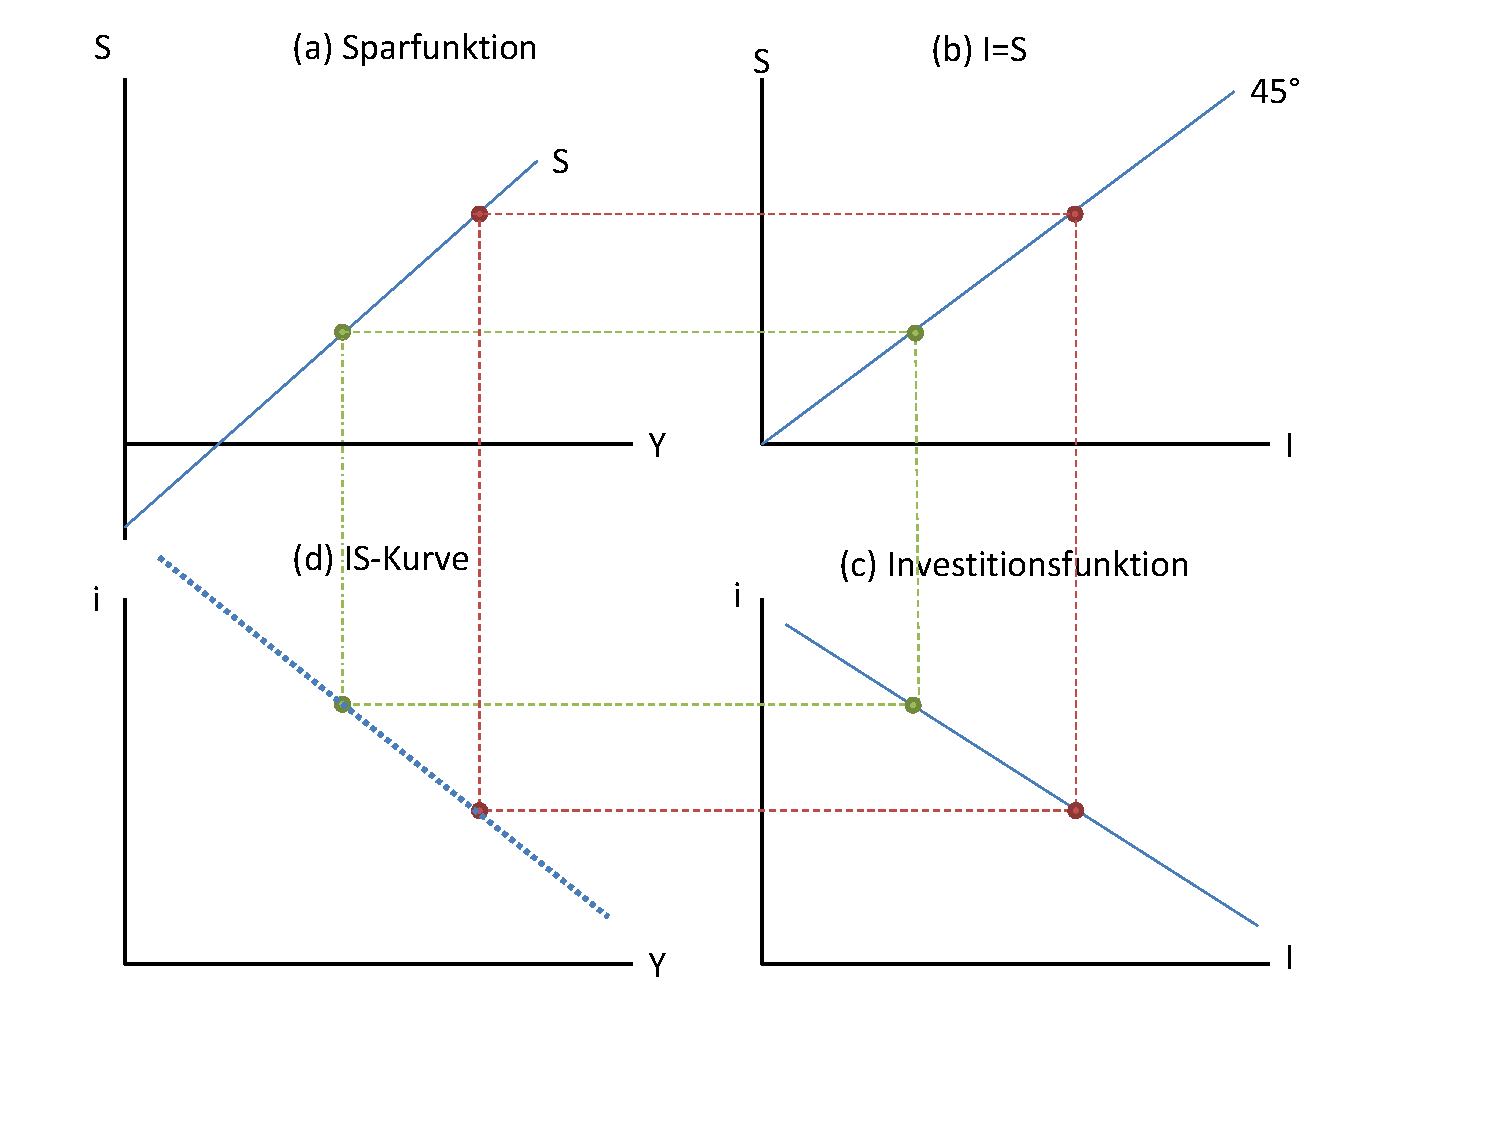
\includegraphics[width=\textwidth]{Bilder/ISgrafisch.pdf}
  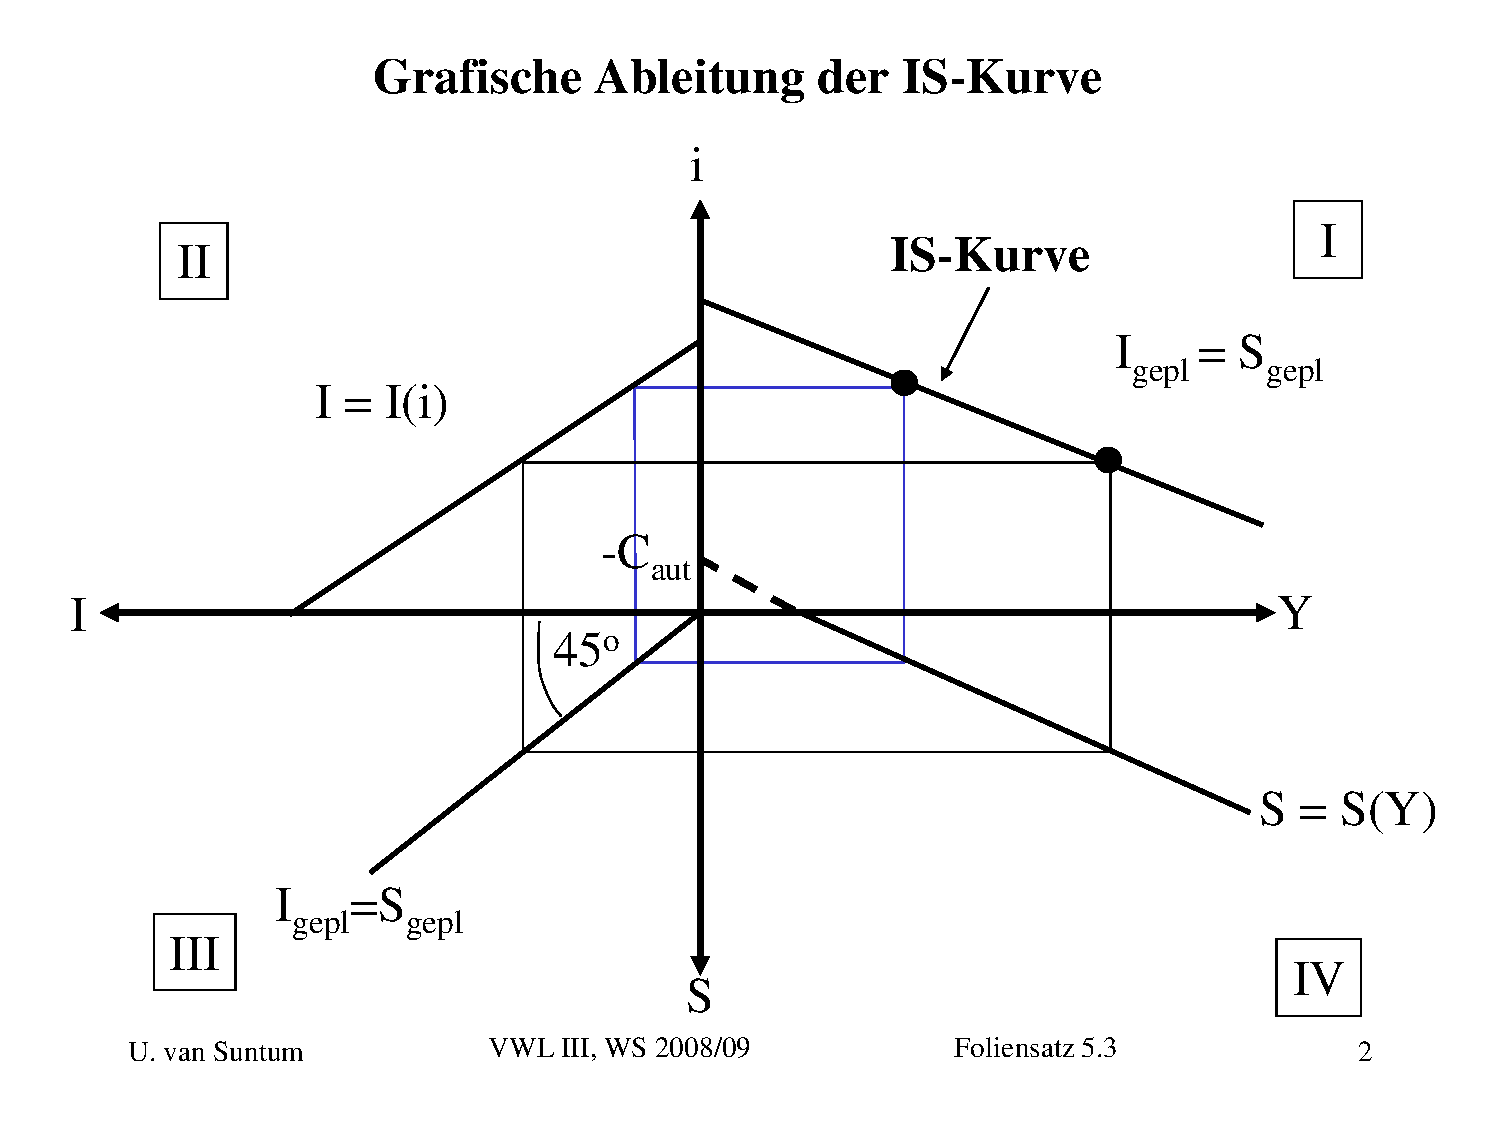
\includegraphics[width=\textwidth]{Bilder/ISgrafisch2.pdf}
\end{center}

\item
\textbf{Steigung der IS-Kurve:}
\begin{align*}
  \frac{\partial r}{\partial Y} = -\frac{1}{b}(1-c_1(1-t))<0
\end{align*}
Interpretation:
\begin{itemize}
  \item Wie stark muss der Zins fallen damit eine Erh\"{o}hung von $Y^*$ um eine marginale Einheit m\"{o}glich ist
  \item $r\downarrow \rightarrow I\uparrow\rightarrow Y \uparrow$
  \item Alternativ: Wie stark muss das Einkommen steigen, damit bei einer Senkung der Zinsen um ein marginales Prozent wieder das Gleichgewicht auf dem G\"{u}termarkt erreicht wird.
\end{itemize}
\textbf{Steigungsparameter:}
\begin{itemize}
\item Zinsabh\"{a}ngigkeit von I (Betrachte relativ gro{\ss}es $b$):
\begin{itemize}
  \item $r\downarrow$
  \begin{itemize}
  \item[$\rightarrow$] starke Erh\"{o}hung von I
  \item[$\rightarrow$] starke Erh\"{o}hung von Y n\"{o}tig, um $S(Y)=I(r)$ wiederherzustellen
  \item[$\rightarrow$] Flache IS-Kurve
  \end{itemize}
\end{itemize}
\item Marginale Konsumneigung (Betrachte relativ hohes $c_1$):
\begin{itemize}
  \item $i\downarrow\rightarrow I\uparrow \rightarrow Y\uparrow \rightarrow S(Y) \uparrow$
  \item Bei hohem $c_1$ gilt, dass h\"{o}heres Y zu geringerer zus\"{a}tzlicher Ersparnis f\"{u}hrt
  \item Multiplikator ist bei hohem $c_1$ gro{\ss}
  \item Flache IS-Kurve
\end{itemize}
\item Steuersatz t (Betrachte relativ hohes t)
\begin{itemize}
  \item Wenn t hoch ist, ist eine geringe Vergr\"{o}{\ss}erung von Y n\"{o}tig, damit $S=I$ wiederhergestellt ist
  \item IS-Kurve verl\"{a}uft steiler fallend
\end{itemize}
\end{itemize}
\textbf{Lageparameter:}
\begin{itemize}
  \item $c_{0} \uparrow, I_{0} \uparrow, G_{0} \uparrow \rightarrow $ Bei gegebenem $r$ f\"{u}hrt dies zu h\"{o}herem Y gem\"{a}{\ss} Multiplikatorprozess
  \item[$\hookrightarrow$] IS-Kurve verschiebt sich nach RECHTS!
  \item $T_{0}\uparrow \rightarrow C\downarrow, Y\downarrow$ bei gegebenem r $\rightarrow$ R\"{u}ckgang G\"{u}ternachfrage
    \item[$\hookrightarrow$] IS-Kurve verschiebt sich nach LINKS!
\end{itemize}
Zusammenfassend: Steuererh\"{o}hungen wirken kontraktiv, Erh\"{o}hung der autonomen Nachfragekomponenten wirken expansiv!

\item
IS-Kurve ordnet jedem Zinssatz ein gleichgewichtiges Einkommen zu.\\
Idee: Jedem Zinssatz ist eine Investitionsnachfrage zugeordnet. Wie hoch muss Y sein, damit die Ersparnis in H\"{o}he der Investitionsnachfrage entsteht.\\
Logik f\"{u}r negative Zinsabh\"{a}ngigkeit vom Zins:\\
Wenn r steigt, sinken die Investitionen. Da diese Bestandteil der effektiven Nachfrage sind, sinkt das Einkommen $Y^*$.\\
Fazit:\\
IS-Kurve bildet das \textbf{simultane} Gleichgewicht auf dem G\"{u}termarkt und dem Kapitalmarkt ab, denn auf dem G\"{u}termarkt ist die geplante Nachfrage gleich dem realisierten Einkommen, w\"{a}hrend auf dem Kapitalmarkt geplante Investitionen im Gleichgewicht der Ersparnis entsprechen!
\end{enumerate}

\subsection{Verst\"{a}ndnisfragen IS-Kurve}
\begin{enumerate}
  \item Wahr!
  \begin{itemize}
  \item Minimalmodel: $d Y = \frac{1}{1-c_1}(d G_{0} + d c_{0})$
  \item Modell mit Steuern: $d Y = \underbrace{\frac{1}{1-c_1(1-t)}}_{Multiplikator}\underbrace{(d G_{0} + d c_{0} - c_1 d T_{0})}_\text{Summe autonomer Gr\"{o}{\ss}en}$
  \end{itemize}
  \item Falsch! $I=S$ und $Y^d=C+I+G$ sind \"{a}quivalent!
  \item Falsch, da Pauschalsteuer in Konsumfunktion eingeht: \\$Y = \frac{1}{1-c_1(1-t)}(\dots+G_{0}-c_1 T_{0}+\dots)$.
\end{enumerate}

\section{Geldmarkt und LM-Kurve}
\subsection{Geldsch\"{o}pfung, Geldnachfrage und Geldangebot}
\begin{enumerate}[(a)]
    \item LM-Kurve: Reale Geldnachfrage = Reales Geldangebot: $(L(\overset{+}{Y},\overset{-}{r})=\frac{M}{P})$
    \begin{enumerate}[(i)]
    \item Geldnachfrage (real): $L(\overset{+}{Y},\overset{-}{i})$
    \begin{itemize}
      \item Transaktionsmotiv:
      \begin{itemize}
      \item Mehr Einkommen $\rightarrow$ Mehr K\"{a}ufe $\rightarrow$ Mehr Geld wird ben\"{o}tigt, d.h. $L_T=L_T(\overset{+}{Y})$, positiv abh\"{a}ngig von Y.
      \end{itemize}
      \item Vorsichtsmotiv:
      \begin{itemize}
      \item Transaktionsbedarf nur begrenzt vorhersehbar
      \item Halte mehr Geld als zu Transaktionszwecken im Durchschnitt n\"{o}tig
      \item Ausgabenschwankungen nehmen mit Ausgaben zu, d.h. $L_V=L_V(\overset{+}{Y})$
      \end{itemize}
      \item Spekulationsmotiv:
        \begin{itemize}
          \item Geld halten statt Wertpapiere, da Kursver\"{a}nderungen mit ber\"{u}cksichtigt werden.
          \item Grundidee: Kapitalmarkt und Wertpapiermarkt stehen in Konkurrenz, Zins verbindet sie
          \begin{itemize}
          \item Kapitalmarkt: $I=S, dB^s=dB^d$ Bondneuemission
          \item Geldmarkt: Alte Bonds werden gehandelt
          \item Verzinsung muss aber identisch sein
          \end{itemize}
          \item Bei uns: Kapitalmarkt wird \"{u}ber G\"{u}termarkt abgebildet und Wertpapiermarkt \"{u}ber Geldmarkt. Da beide zusammenwirken, folgt identischer Zins.
          \item $i\uparrow$, d.h. mehr Leute glauben, dass Zins und Kursver\"{a}nderungen eines Wertpapiers gr\"{o}{\ss}er als Null sind und wollen mehr Wertpapiere als Geld halten $\rightarrow L_S=L_S(\overset{-}{i})$
        \end{itemize}
        \item Somit: $L = L_T(\overset{+}{Y})+L_V(\overset{+}{Y})+L_S(\overset{-}{i}) = L(\overset{+}{Y},\overset{-}{i})$
    \end{itemize}

    \item Geldangebot (nominal), $M^s=M$
    \begin{itemize}
      \item Exogen gegeben, da von Zentralbank kontrolliert!
      \item Wie macht die Zentralbank das?
      \begin{itemize}
      \item Offenmarktpolitik [bzw. evtl. durch Mindestreservesatz]
      \item Offenmarktpolitik: Ankauf oder Verkauf von Wertpapieren (bzw. Repos)
      \item Idee:
      \begin{itemize}
        \item ZB kauft Wertpapiere, bezahlt mit Geld $(M\uparrow)$
        \item ZB verkauft Wertpapiere, bekommt Geld $(M\downarrow)$
      \end{itemize}
      \item Genauer: Negativer Zusammenhang zwischen Kurs und aktuellem Zins eines Wertpapiers aufgrund von Arbitrage:
      \begin{align*}
        (1+r)P_B = \underbrace{NW\cdot(1+r_0)}_\text{konstant}
      \end{align*}
      \item D.h. wenn ZB Wertpapiere nachfragt, steigt $P_B$, da $NW\cdot(1+r_0)$ konstant ist, muss $r$ sinken: $P_B\uparrow \rightarrow r \downarrow$
      \item Bei gegebenem $Y$ folgt $r\downarrow \rightarrow L(Y,\overset{-}{r})\uparrow$, da $\frac{\partial L}{\partial r}<0$. Daraus folgt $M\uparrow$.
      \item In der Realit\"{a}t ist die Zentralbank aber nur begrenzt f\"{a}hig, $M$ zu steuern aufgrund der Geldsch\"{o}pfung der Gesch\"{a}ftsbanken
      \end{itemize}
    \end{itemize}
    \item Gleichgewicht: $M^s=M^d $
    \begin{align*}
      \Leftrightarrow \underbrace{\frac{M}{P}}_\text{konstant}=L(\overset{+}{Y},\overset{-}{r})
    \end{align*}
    \begin{itemize}
      \item Aufgrund des exogenen Geldangebots muss auch die Geldnachfrage konstant sein!
      \item Wenn Y steigt, muss r auch steigen! $\rightarrow$ Positive Steigung der LM-Kurve!
      \item $Y\uparrow\rightarrow (L_T+L_V)\uparrow$, d.h. Subjekte brauchen mehr Geld, also wollen sie Wertpapiere verkaufen $\rightarrow P_B \downarrow \rightarrow r \uparrow \rightarrow L_r \downarrow$, d.h. Wertpapierkauf wird immer unattraktiver und die Geldnachfrage kehrt zum urspr\"{u}nglichen Niveau zur\"{u}ck.
    \end{itemize}
  \end{enumerate}
  \item Geldmarkt:
  \begin{center}
  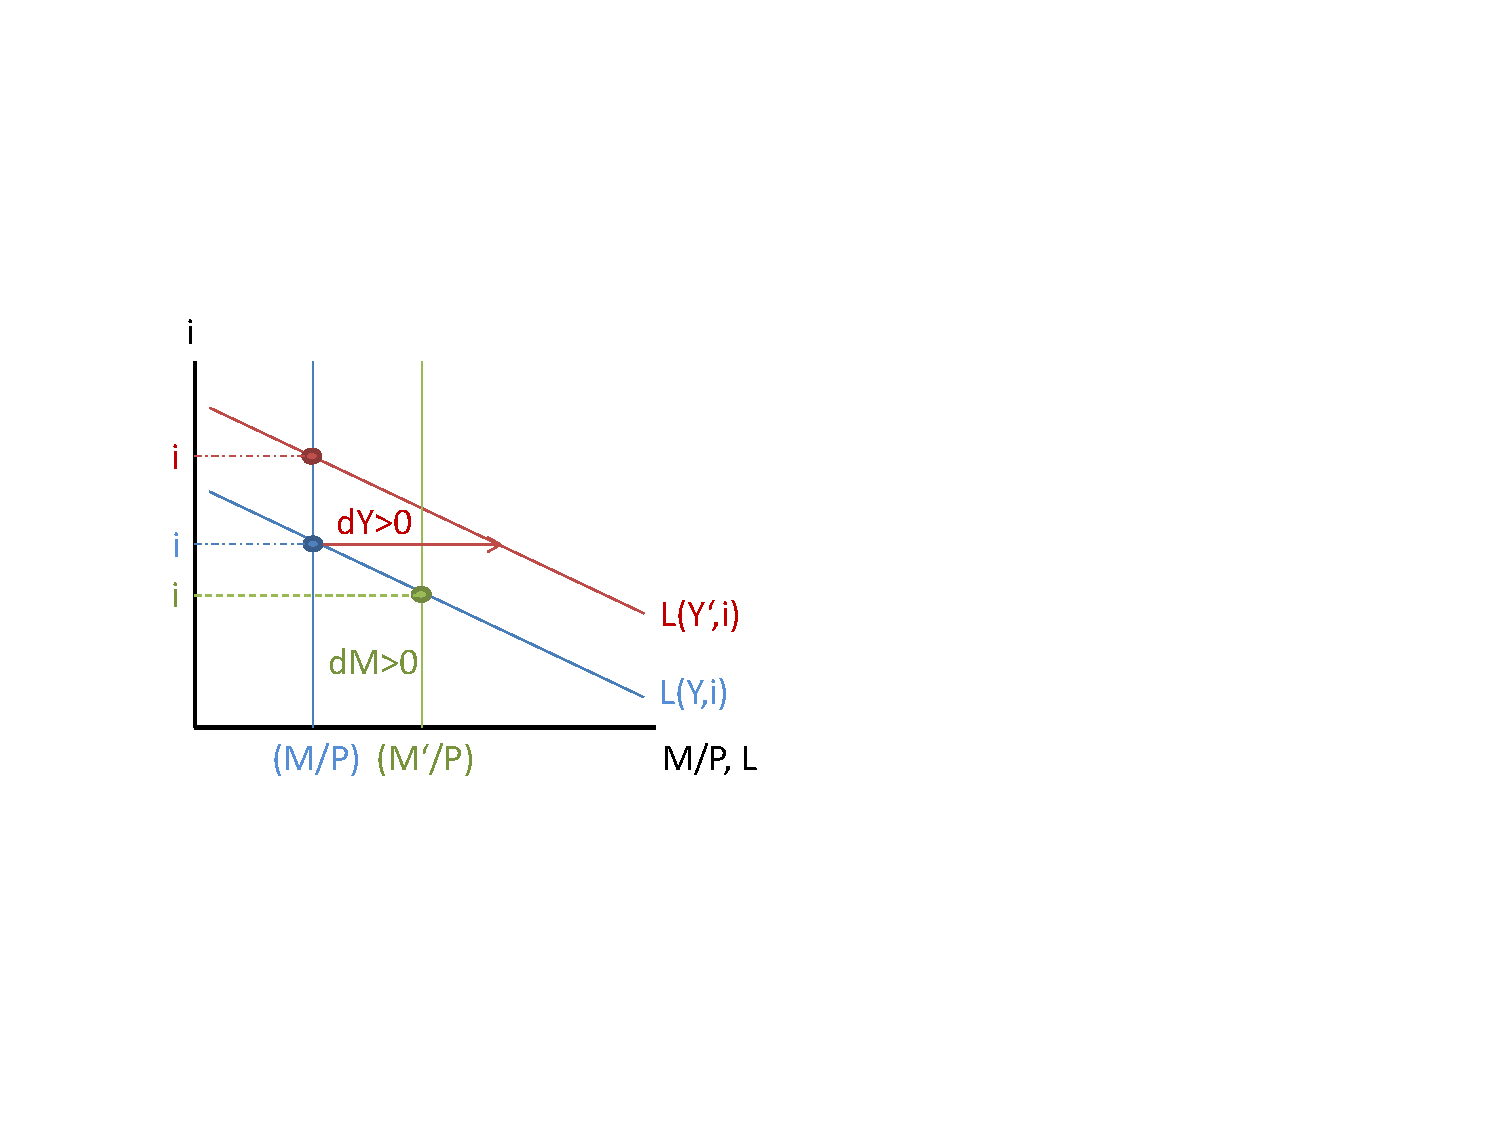
\includegraphics[width=.5\textwidth]{Bilder/geldmarkt.pdf}
  \end{center}
  Ver\"{a}nderungen:
  \begin{itemize}
    \item $Y \uparrow \rightarrow$ Rechtsverschiebung der Geldnachfrage, d.h. $r\uparrow$
    \item $M\uparrow$ bzw. $P \downarrow \rightarrow$ Rechtsverschiebung des Geldangebots, d.h. $r \downarrow$
  \end{itemize}
  \item Herleitung LM-Kurve:
  \begin{itemize}
    \item Grafisch:
  \begin{center}
  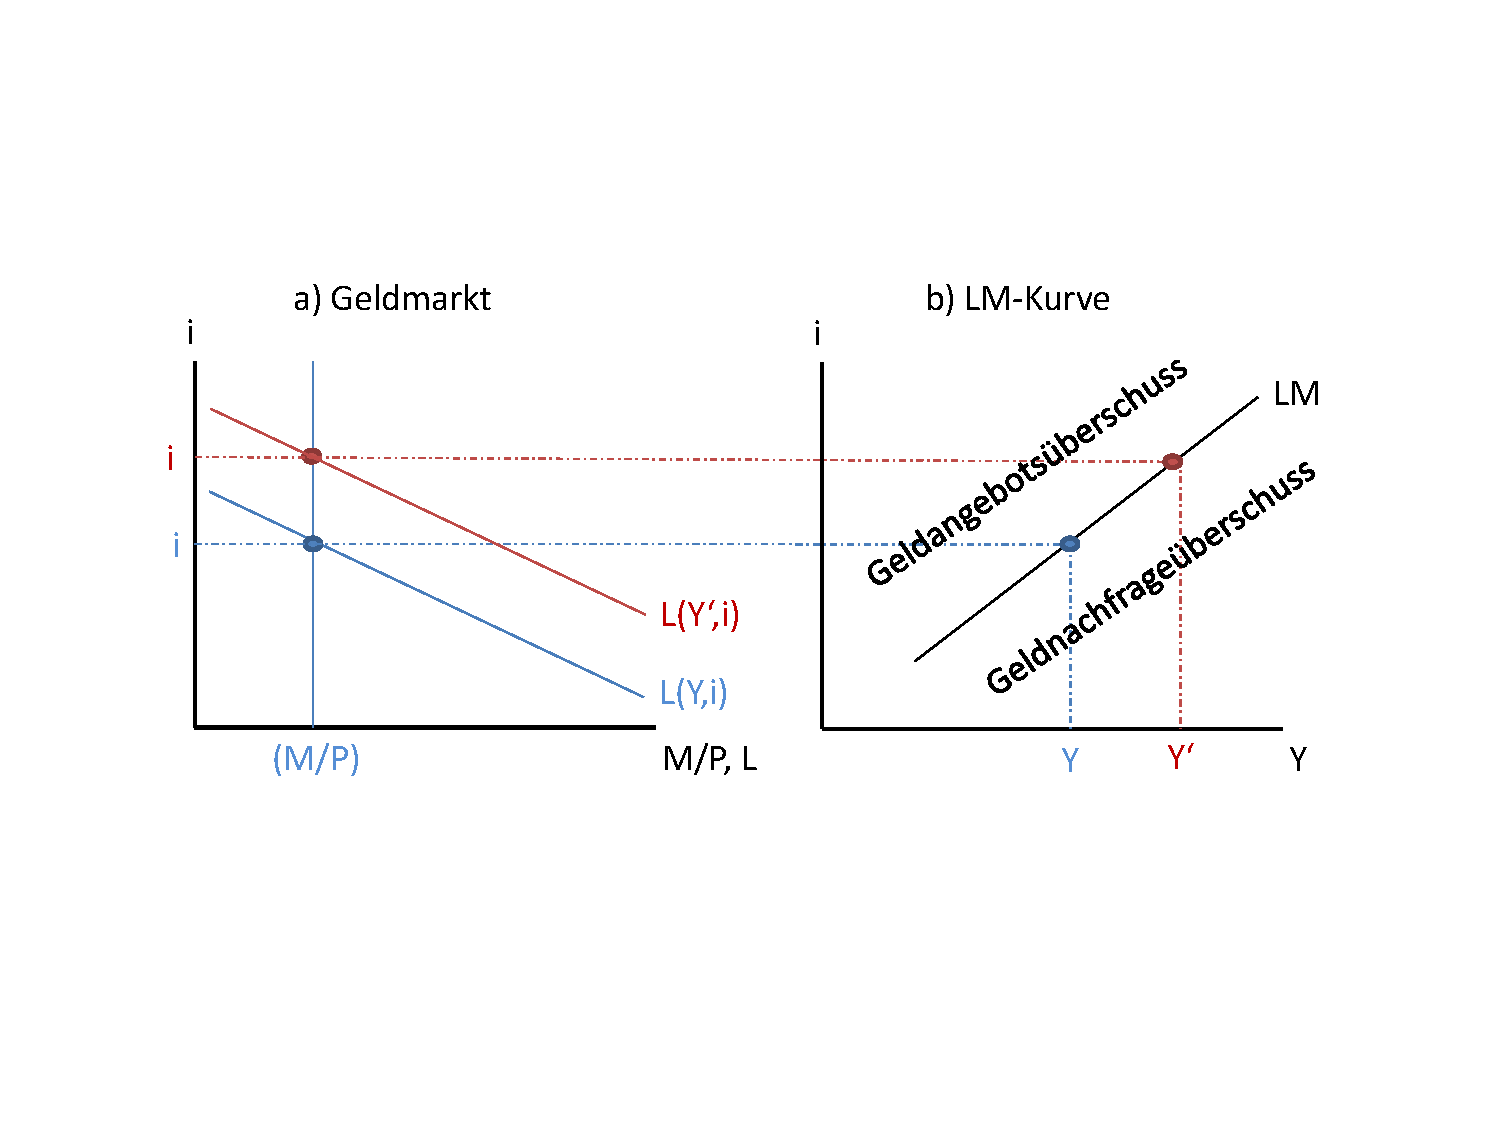
\includegraphics[width=\textwidth]{Bilder/LM.pdf}\\
    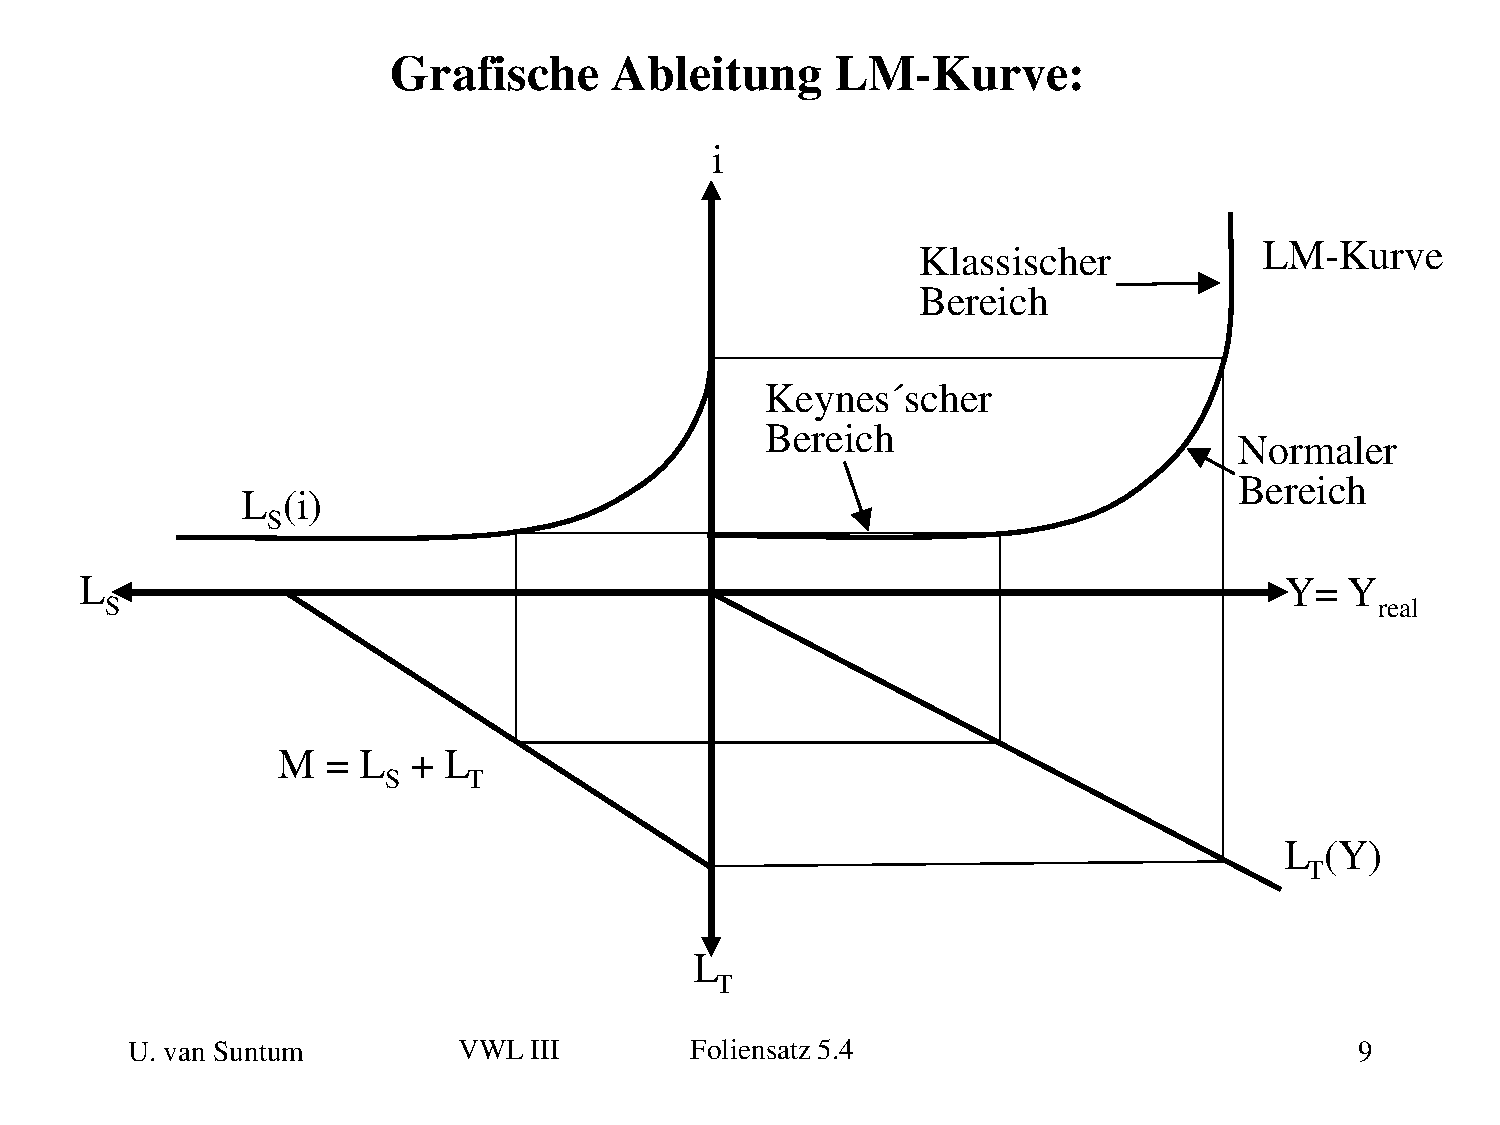
\includegraphics[width=\textwidth]{Bilder/LM2.pdf}
  \end{center}
    \item Analytisch:
    \begin{align*}
      \frac{M}{P}= L(Y,r)
    \end{align*}
    Hier kommt es auf die funktionale Form von L an, einfach nach Y oder r aufl\"{o}sen.
  \end{itemize}
  \item
  \begin{itemize}
    \item Steigung:
  \begin{align*}
    \frac{M}{P}&= L(Y,r)\\
    \frac{1}{P}dM - \frac{M}{P^2}dP &= \overset{>0}{L_Y} dY + \overset{<0}{L_r} dr
  \end{align*}
  F\"{u}r Steigung: $dM=dP=0$:
  \begin{align*}
    \frac{dY}{dr}=-\frac{L_Y}{L_r}>0
  \end{align*}
   \item Zinsabh\"{a}ngigkeit von L, betrachte also $L_r$:
   \begin{itemize}
     \item hohes $|L_r| \rightarrow$ Flacher Verlauf der  LM-Kurve
     \item niedriges $|L_r| \rightarrow$ Steiler Verlauf der LM-Kurve
     \item Klassik: $L_r=0 \rightarrow$ Senkrechte LM-Kurve
     \item Liquidit\"{a}tsfalle $L_r= -\infty \rightarrow$ horizontale LM-Kurve
   \end{itemize}
   \item Einkommensabh\"{a}nigkeit der Geldnachfrage, betrachte also $L_Y$
   \begin{itemize}
     \item Hohes $L_Y, Y\uparrow \rightarrow L\upuparrows$, d.h. starke Zinserh\"{o}hung erforderlich, um Geldnachfrage wieder auf das Niveau der realen Geldmenge zu bringen $\rightarrow$ Steile LM-Kurve
   \end{itemize}
   \item Lageparameter (Verschiebung der LM-Kurve)
   \begin{align*}
       \frac{1}{P}dM - \frac{M}{P^2}dP &= \overset{>0}{L_Y} dY + \overset{<0}{L_r} dr
       \end{align*}
  \begin{itemize}
     \item Erh\"{o}hung von $M (dr=dP=0)$
     \begin{align*}
       \frac{dY}{dM}=\frac{1}{P L_Y} >0
     \end{align*}
     $\rightarrow$ Rechstverschiebung, zu jedem Outputniveau ist nun ein h\"{o}heres Zinsniveau erforderlich
     \item Erh\"{o}hung von $P (dr=dM=0)$
     \begin{align*}
       \frac{dY}{dP}=\frac{-M}{P^2 L_Y} <0
     \end{align*}
     $\rightarrow$ Linksverschiebung
   \end{itemize}
  \end{itemize}
  \item LM-Kurve ist der geometrische Ort aller Kombinationen aus Zinsen und Einkommen, f\"{u}r die der Geldmarkt im Gleichgewicht ist.
\end{enumerate}

\subsection{Geldsch\"{o}pfungsmultiplikator}
\begin{enumerate}[1)]
  \item Geldmenge = Cash + Einlagen | $M=C+E \Leftrightarrow E=M-C$
  \item Bargeldquote = Cash/Geldmenge | $c = C/M \Leftrightarrow C=cM$
  \item Mindestreservesatz = Reserven/Einlagen | $r=RE/E \Leftrightarrow RE =rE = r(M-C) \Leftrightarrow RE = r(M-cM) = r(1-c)M$
  \item Geldbasis = Cash +Reserven | $B=C+RE = cM + r(1-c)M \Leftrightarrow M = \frac{1}{c+r(1-c)}(C+RE) = mB$
\end{enumerate}
Hier m=5.78!
\subsection{Verst\"{a}ndnisfrage LM}
\begin{enumerate}[1)]
  \item wahr
  \item wahr
  \item wahr
  \item wahr
  \item falsch
  \item falsch (Wertaufbewahrung)
\end{enumerate}

\section{IS-LM Modell}

\subsection{Wirtschaftspolitische Ma{\ss}nahmen}
Herleitung IS (G\"{u}termarkt-GG):
\begin{align*}
  Y^d=Y^s=Y &= C+I+G = c_{0} + c_1(Y-T_{0}) + I_{0}-br + G_{0}\\
  Y &= \frac{1}{1-c_1}(c_{0} - c_1T_{0} + I_{0}-br + G_{0})\\
  \text{Totales Differential:}\\
  dY &= \frac{1}{1-c_1}(dc_{0}-c_1 dT_{0} + dI_{0} - b dr + dG_{0})
\end{align*}
Herleitung LM (Geldmarkt-GG):
\begin{align*}
  M = M^a = P L \Leftrightarrow \frac{M}{P} &= L(Y,r)\\
  \text{Totales Differential:}\\
  \frac{1}{P}dM - \frac{M}{P^2}dP &= L_Y dY + L_r dr\\
  \Leftrightarrow dr &= \frac{1}{L_r} \left(\frac{1}{P}dM-\frac{M}{P^2}dP-L_Y dY\right)
\end{align*}
LM in IS einsetzen, und Terme zusammenfassen
\begin{align*}
  dY = \frac{1}{1-c_1 -\frac{b L_Y}{L_r}} \left(dc_{0} - c_1 dT_{0} + dI_{0} +dG_{0} - \frac{b}{L_r} \left(\frac{1}{P}dM-\frac{M}{P^2}dP\right)\right)
\end{align*}
\begin{enumerate}
  \item Steuerfinanzierte Staatsausgabenerh\"{o}hung
  \begin{align*}
    dG_{0}&=dT_{0}>0; dM_{0}=dI_{0}=dc_{0}=dP=0, P=1\\
  dY &= \frac{1}{1-c_1 -\frac{b L_Y}{L_r}} \left(- c_1 \underbrace{dT_{0}}_{=dG_{0}} +dG_{0} \right) = \frac{\overbrace{1-c_1}^{>0}}{\underbrace{\overbrace{1-c_1}^{>0} - \overbrace{\frac{b L_Y}{L_r}}^{<0}}_{>0}} \underbrace{dG_{aut}}_{>0} >0\\
  dr &= \underbrace{\frac{-L_Y}{L_r}}_{>0} \underbrace{dY}_{>0} >0
  \end{align*}
  Eine Steuerfinanzierte Staatsausgabenherh\"{o}hung erh\"{o}ht Y und r --> Expansive Wirkung\\
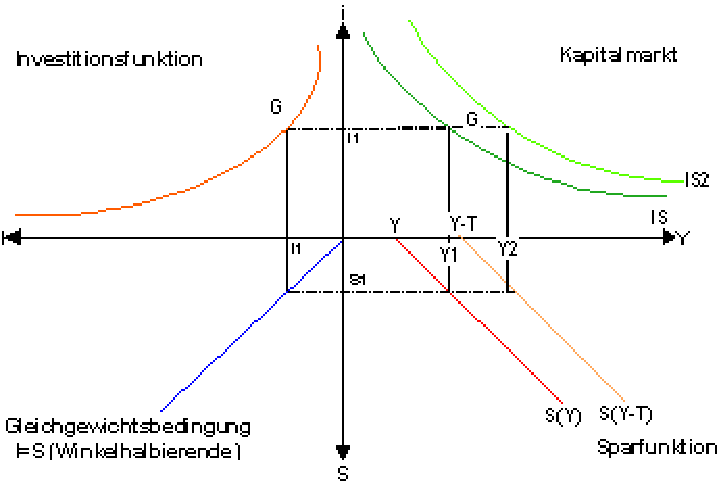
\includegraphics[width=0.5\textwidth]{Bilder/ISLMSteuerfinanziert.pdf}\\
Durch Steuern wird die Sparfunktion um T(=G) verschoben; Bei einem konstanten Zins $r_1$ und einer Konstanten Sparleistung $S_1$ mu{\ss} sich jetzt das Einkommen erh\"{o}hen von $Y_1$ auf $Y_2$. Daher verschiebt sich die IS-Kurve genau um G nach au{\ss}en und das Einkommen steigt ebenfalls um $G=Y_2-Y_1$. Grund der Einkommenssteigerung ist die marginale Konsumneigung.\\
Fazit: Kampf gegen Arbeitslosigkeit m\"{o}glich ohne Budgetbelastung!\\
Haavelmo Theorem:\\
Expanisve Wirkung das das Einkommen k\"{o}nnen von einem ausgeglichenem Staatshaushalt ausgehen (Mehr Steuer, diese Einnahmen sofort ausgeben). Grund: Staat besitzt im Gegensatz zu den privaten Haushalten keine marginale Sparquote, somit werden Steuereinnahmen zu 100\% Nachfragewirksam.
  \item Kreditfinanzierte Steuersenkung
  \begin{align*}
    dT_{0}<0; dM_{0}=dI_{0}=dc_{0}=dG_{0}=dP=0, P=1\\
  dY = \frac{1}{1-c_1 -\frac{b L_Y}{L_r}} \left(- c_1 \underbrace{dT_{0}}_{<0}\right) >0\\
  dr = \frac{-L_Y}{L_r} dY >0
  \end{align*}
  Eine Kreditfinanzierte Steuersenkung erh\"{o}ht Y und r; Wirkung umso st\"{a}rker, je h\"{o}her die marginale Konsumneigung ist.\\
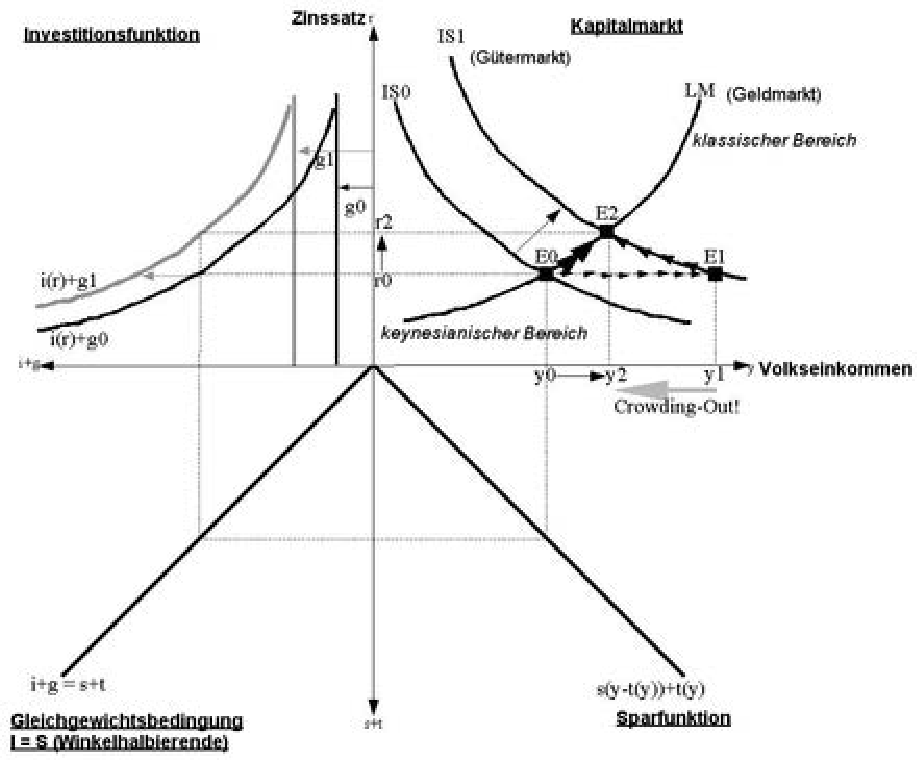
\includegraphics[width=0.5\textwidth]{Bilder/ISLMKreditfinanzierteSteuersenkung.pdf}\\
Wirkungskette: $T\downarrow \rightarrow C\uparrow \rightarrow Y^d \uparrow \rightarrow Y^d > Y^s \rightarrow Y \uparrow$ (G\"{u}termarkt, IS Kurve verschiebt sich nach rechts), $Y\uparrow \rightarrow L > M^s/P \rightarrow P_B \downarrow \rightarrow i \uparrow I \downarrow \rightarrow Y^d \downarrow \dots bis Y^d = Y = Y^s.$ (Bewegung AUF der IS Kurve).
\item Erh\"{o}hung der autonomen Investitionen
  \begin{align*}
    dI_{0}>0; dM_{0}=dT_{0}=dC_{0}=dG_{0}=dP=0, P=1\\
  dY &= \frac{1}{1-c_1 -\frac{b L_Y}{L_r}} \left(\underbrace{dI_{0}}_{>0}\right) >0\\
  dr &= \frac{-L_Y}{L_r} dY >0
  \end{align*}
  Grafik v\"{o}llig analog zu Kreditfinanzierten Staatsausgabenerh\"{o}hungen.\\
  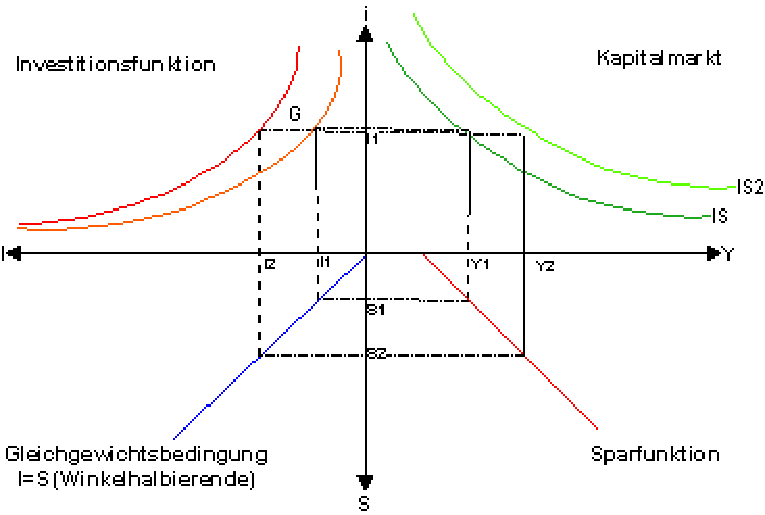
\includegraphics[width=0.5\textwidth]{Bilder/ISLMKreditfinanziert.pdf}\\
\item Erh\"{o}hung des Geldangebots: $dM>0$ (oder Senkung des Preisniveaus $dP<0$)
\begin{align*}
    dY &= \frac{1}{1-c_1 -\frac{b L_Y}{L_i}} \left(- \frac{b}{L_i} \frac{1}{P}dM\right) >0\\
    di &= \frac{1}{L_i P} dM-\frac{L_Y}{L_i} dY = \frac{1}{L_i}\left(\frac{dM}{P}-L_Y \frac{1}{1-c_1 -\frac{b L_Y}{L_i}} \left(- \frac{b}{L_i} \frac{1}{P}dM\right) \right)\\
    di &= \frac{1}{L_i}\left(1 + \frac{\frac{b L_Y}{L_i}}{1-c_1-\frac{b L_Y}{L_i}}\right) \frac{dM}{P} =\frac{1}{L_i}\left(\frac{ 1-c_1-\frac{b L_Y}{L_i} + \frac{b L_Y}{L_i}}{1-c_1-\frac{b L_Y}{L_i}}\right) \frac{dM}{P}<0
\end{align*}
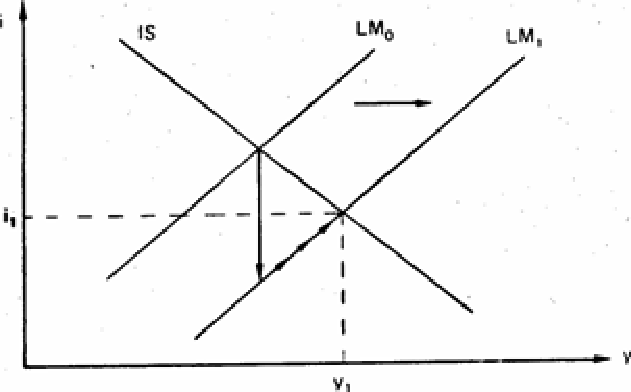
\includegraphics[width=0.5\textwidth]{Bilder/ISLMGeldpolitik.pdf}\\
Zusammenfassend:\\
Korrelation zwischen Zins und Einkommen h\"{a}ngt von der Politikma{\ss}nahme ab:
\begin{itemize}
  \item Fiskalpolitik oder Investitionspolitik gibt positive Korrelation
  \item Geldpolitik gibt negative Korrelation
\end{itemize}
\end{enumerate}

\subsection{Rechenaufgabe}
\begin{enumerate}
  \item \begin{align*}
    Y^s=Y^d \Leftrightarrow Y = C + I + G = \frac{1}{5}Y + 60 \Leftrightarrow Y^* = 75
  \end{align*}
  \item \begin{align*}
    dY &= \frac{-c}{1-c(1-q)} dT_{aut} = \frac{-1/2}{4/5} dT_{aut} = -5\\
    dT^* &= d^T_{aut} + \frac{3}{5}dY = 5
  \end{align*}
  \item \begin{align*}
    \text{IS: } Y &= \frac{1}{5}Y + 70 -40 i; C=\frac{1}{5}Y\\
    \text{LM: } \frac{M}{P} &= L \Leftrightarrow11.5 = \frac{1}{5}Y -30i = C-30i\\
    \text{IS: } \frac{4}{5} Y &= 70-40i\\
    C=\frac{1}{5}Y &= \frac{70}{4}-10i = 11.5 + 30i = \frac{46}{4}+30i \Leftrightarrow 6 = 40i\\
    \Rightarrow \frac{4}{5} Y &= 4 C = 70-6 = 64 \Rightarrow C^*=16
  \end{align*}
\end{enumerate}

\subsection{Verst\"{a}ndnisfragen IS-LM}
\begin{enumerate}
  \item Falsch
  \item Wahr
  \item Wahr
  \item Wahr
  \item Wahr
  \item Falsch
\end{enumerate}

\section{Offene Volkswirtschaft und Mundell-Fleming}
\subsection{Offene Volkswirtschaft}
\begin{enumerate}[a)]
\item Zentraler Unterschied: Gesamtwirtschaftliche inl\"{a}ndische Nachfrage muss nicht mehr gleich dem inl\"{a}ndischen Angebot an G\"{u}tern und Dienstleistungen sein. G\"{u}ter k\"{o}nnen vom Ausland importiert und ins Ausland exportiert werden. Zahlungsbilanz erfasst alle Transaktionen zwischen Inl\"{a}ndern und Ausl\"{a}ndern; sie ist das buchhalterische Abbild des Devisenmarkts.\\
    Devisenmarkt:
    \begin{itemize}
      \item Angebot an Fremdw\"{a}hrung: Bestimmt durch Export bzw. Kapitalimport
      \item Nachfrage nach Fremdw\"{a}hrung: bestimmt durch Import bzw. Kapitalexport
      \item Wechselkurs ist Preis zwischen ausl\"{a}ndischer und inl\"{a}ndischer W\"{a}hrung ($S = \frac{inl\"{a}nd.W\"{a}hrung}{ausl. W\"{a}hrung}=\frac{Euro}{Dollar}$), der den Devisenmarkt ins Gleichgewicht bringt.
    \end{itemize}
\begin{center}
  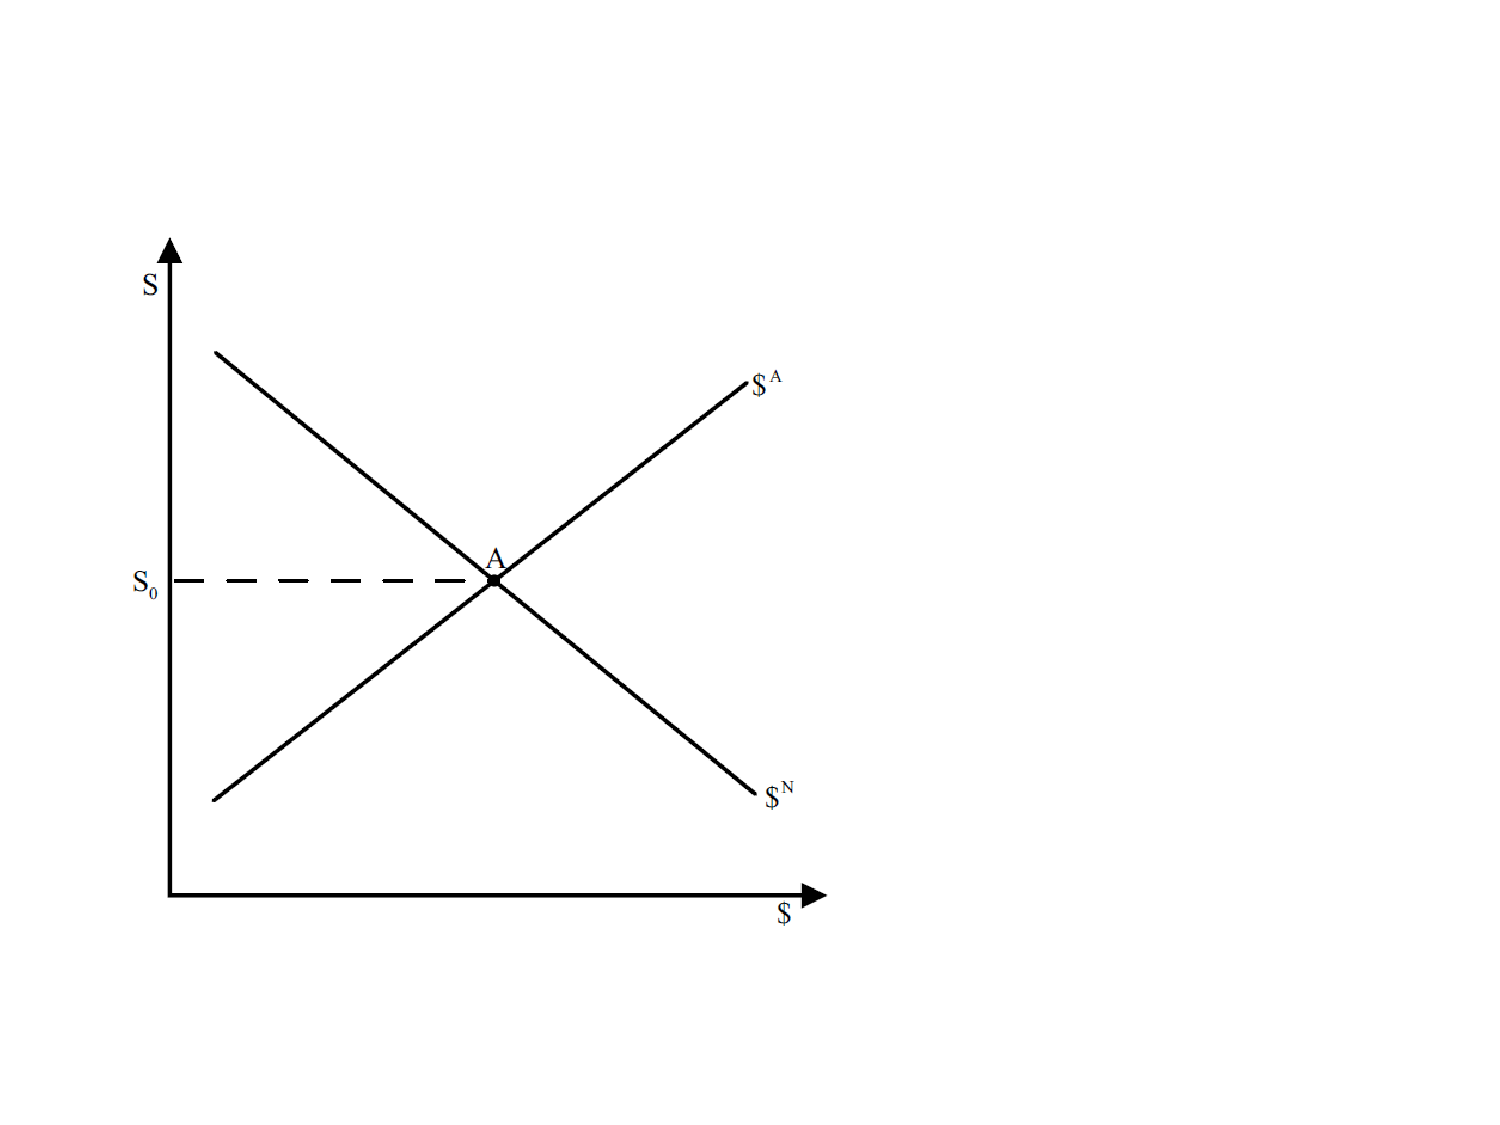
\includegraphics[width=0.5\textwidth]{Bilder/Devisenmarkt.pdf}
\end{center}
\begin{itemize}
  \item Fallende Nachfrage: $S\uparrow \rightarrow$ H\"{o}here Importpreise, d.h. Inland fragt weniger Importg\"{u}ter nach $IM \downarrow \rightarrow$ Dollarnachfrage sinkt ($\$^{N}\downarrow$)!
  \item Steigendes Angebot: $S\uparrow \rightarrow$ Abwertung inl\"{a}ndischer W\"{a}hrung $\rightarrow$ Inl\"{a}ndische G\"{u}ter werden g\"{u}nstiger $\rightarrow$ EX $\uparrow \rightarrow$ Dollarangebot steigt ($\$^{A}\uparrow$)!
\end{itemize}
\item Vereinfachend bei uns:
\begin{align*}
  Handelsbilanzssaldo &= Leistungsbilanzsaldo\\
  \underbrace{S-I}_\text{Nettokapitalabfl\"{u}sse} &= \underbrace{EX-IM}_\text{Nettoexporte}
\end{align*}
\begin{center}
$S>I$ Nettodarlehensgeber | $EX-IM >0$ LB-\"{U}berschuss\\
$S<I$ Nettodarlehensnehmer | $EX-IM <0$ LB-Defizit\\
internationaler Finanzstrom | internationaler G\"{u}terstrom
\end{center}
Ein LB-Defizit erfordert einen Kapitalzufluss zur Finanzierung der Nettoimporte!
\end{enumerate}

\subsection{Mundell Fleming}
\begin{enumerate}[a)]
  \item Gleichungen:
  \begin{itemize}
    \item IS- Kurve: GG auf G\"{u}termarkt und Kapitalmarkt
    \begin{align*}
      Y = C(\overset{+}{Y}) + I(\overset{-}{i}) + G + X(\overset{+}{Y^*},\overset{+}{S}) - IM(\overset{+}{Y},\overset{-}{S})
    \end{align*}
    \item LM-Kurve: GG auf Geldmarkt
    \begin{align*}
      M= D+R = L(\overset{+}{Y},\overset{-}{i})
    \end{align*}
    \item ZZ- Kurve: geometrischer Ort aller (i,Y) Kombinationen f\"{u}r die der Devisenmarkt im GG ist
    \begin{align*}
       \underbrace{X(\overset{+}{Y^*},\overset{+}{S}) - IM(\overset{+}{Y},\overset{-}{S})}_\text{Leistungsbilanz} + \underbrace{F(\overset{+}{i},\overset{-}{i^*})}_\text{Handelsbilanz} = 0
    \end{align*}
    F: Nettokapitalimporte als Saldo aus Direktinvestitionen, Wertpapiertransaktionen und dem \"{u}brigen Kapitalverkehr
    $F>0$ Nettokapitalimport, $F<0$ Nettokapitalexport
\begin{center}
  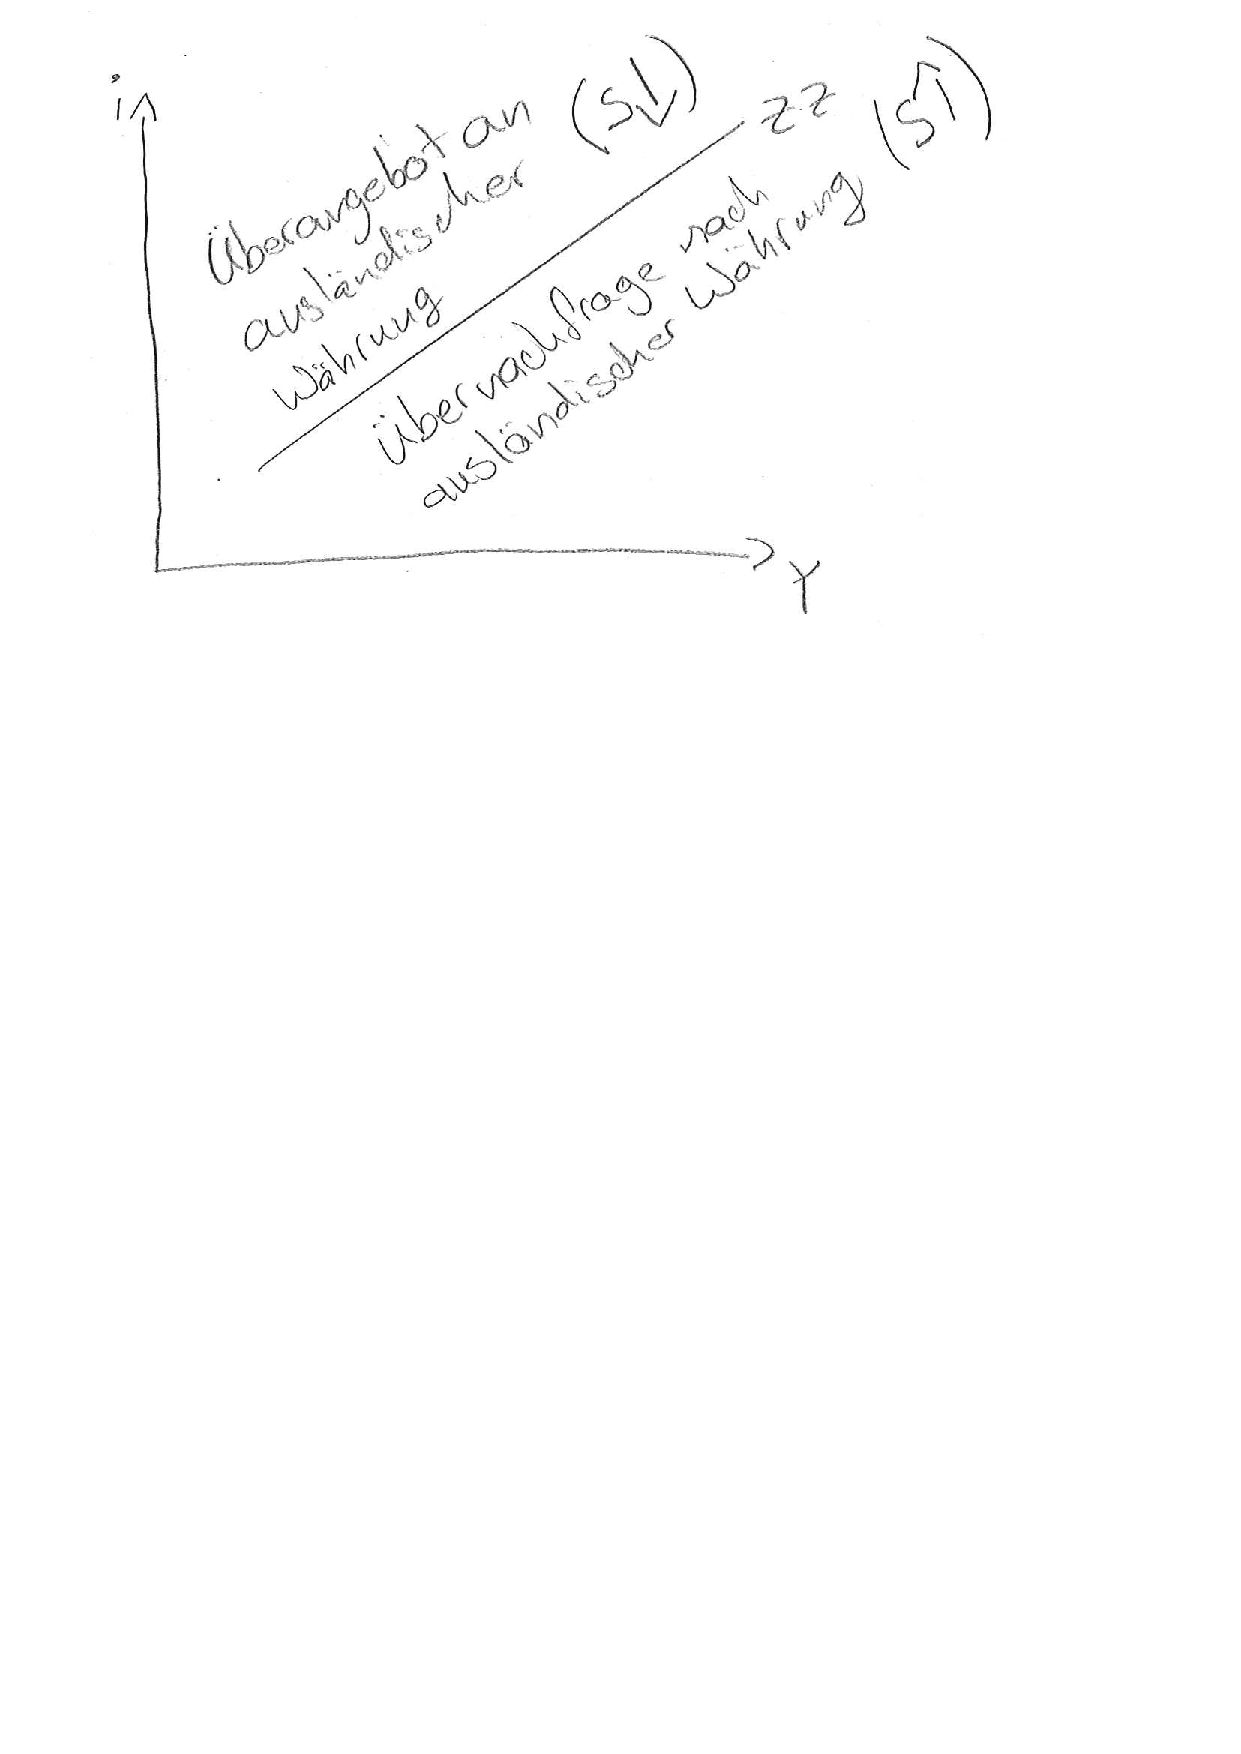
\includegraphics[width=0.5\textwidth]{Bilder/ZZObenUnten.pdf}
\end{center}
\begin{center}
  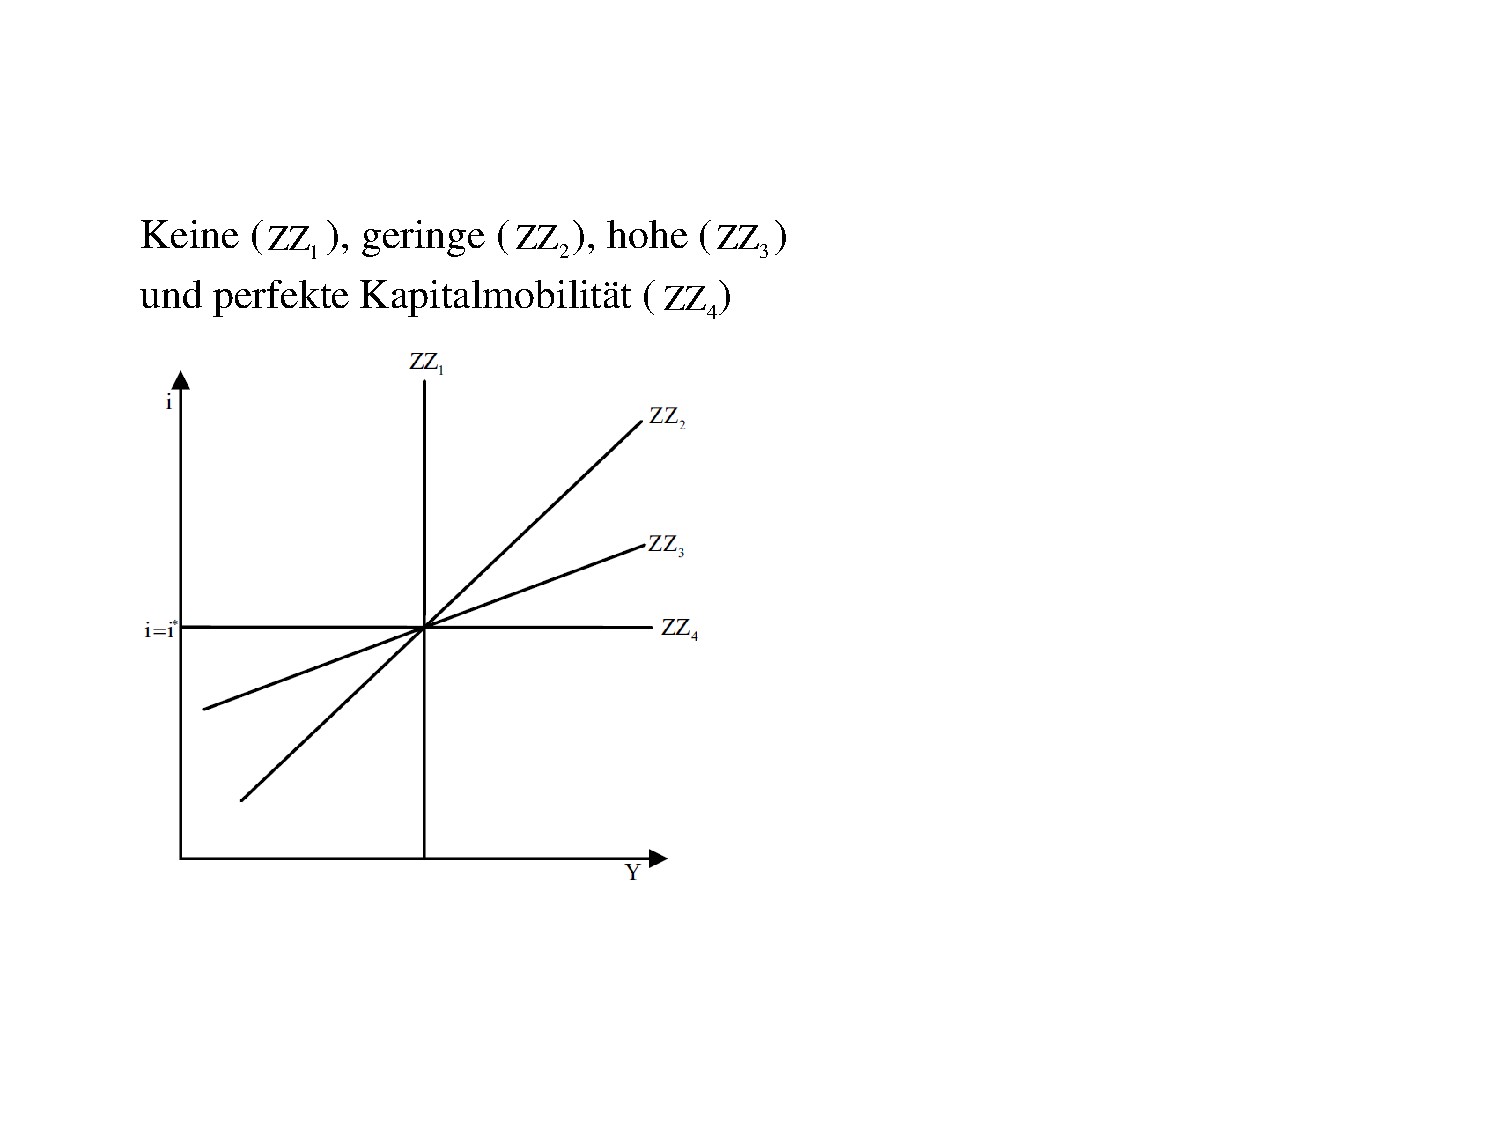
\includegraphics[width=0.5\textwidth]{Bilder/ZZSteigung.pdf}
\end{center}
\begin{center}
  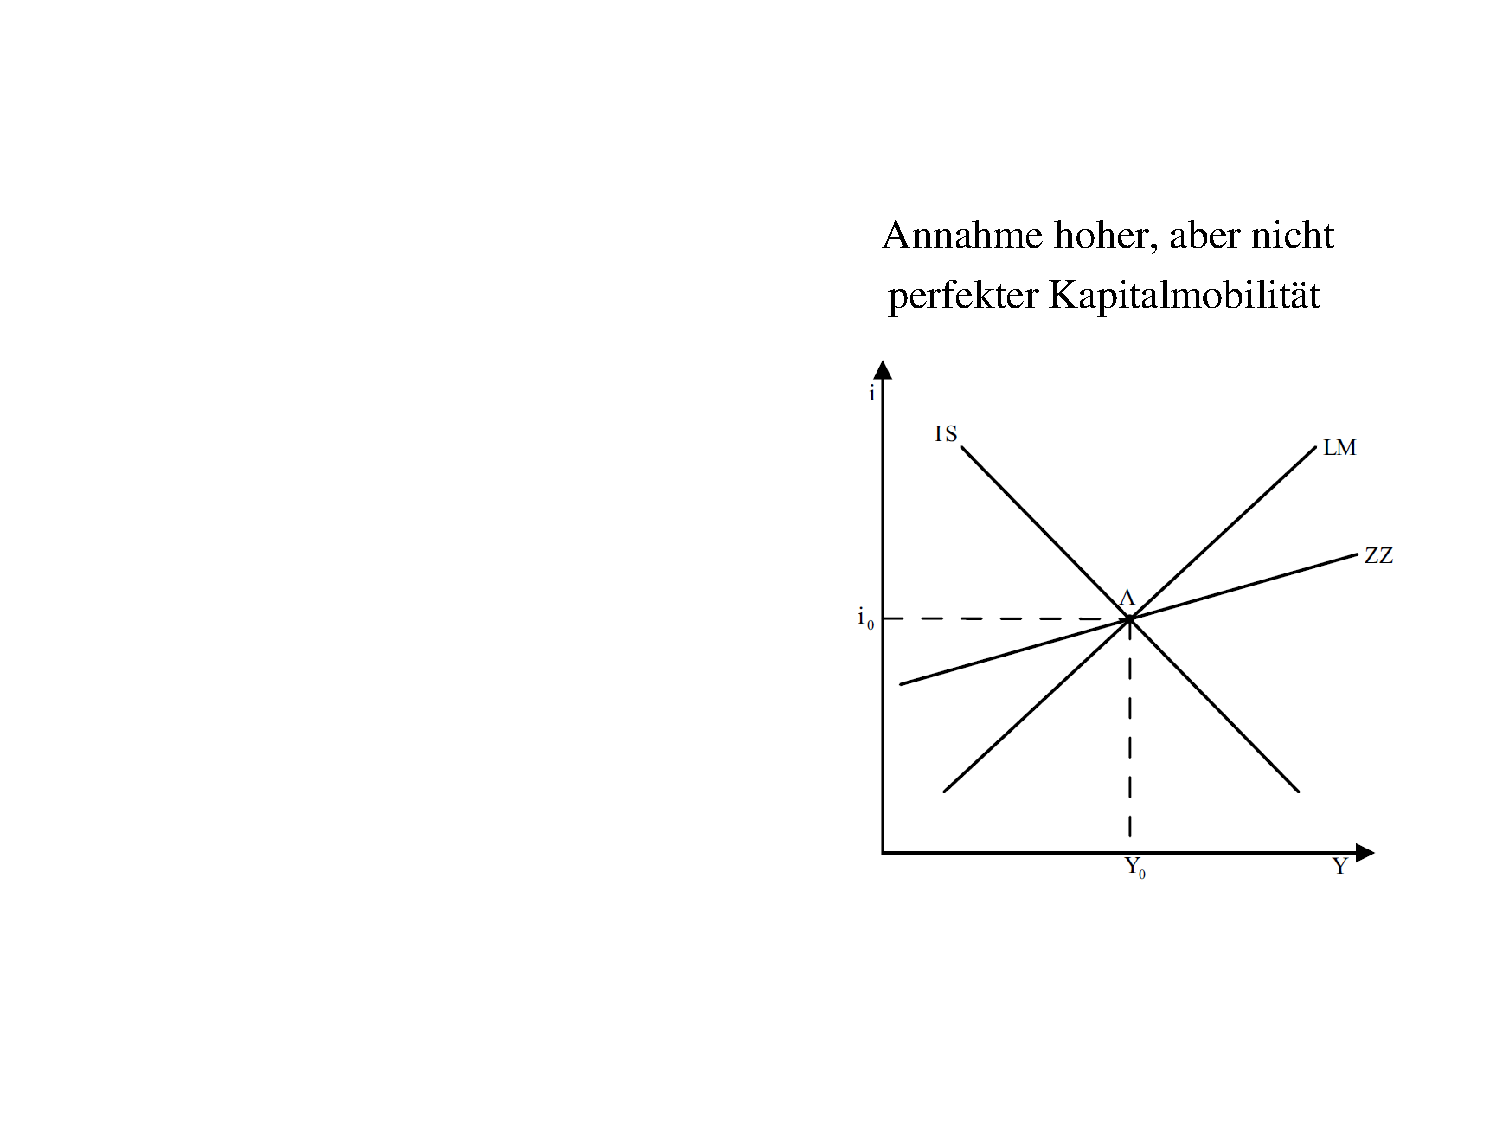
\includegraphics[width=0.5\textwidth]{Bilder/ZZISLM.pdf}
\end{center}
    Steigung h\"{a}ngt von Kapitalmobilit\"{a}t ab: ZZ-Kurve verl\"{a}uft flacher als LM-Kurve, wenn F stark zinselastisch ist, also hohe Kapitalmobilit\"{a}t vorliegt. Bei perfekter Kapitalmobilit\"{a}t gilt $i=i^*$.
  \item LAGE: S und $i^*$
  \begin{align*}
    S\uparrow \begin{cases}\begin{rcases}
    \rightarrow X \uparrow, \text{ da Inlandsg\"{u}ter im Ausland billiger werden } \rightarrow \$^{A} \uparrow\\
    \rightarrow IM\downarrow \rightarrow \$^{N} \downarrow
    \end{rcases}\end{cases}
    \Rightarrow \$^{A} > \$^{N}
  \end{align*}
  Devisenangebots\"{u}berschuss!. Bei gegebenem Y muss i nun solange fallen, bis \"{U}berschussangebot weg ist, d.h. Verschiebung nach rechts unten!
  \\~\\
  $i^*$: F\"{u}r gegebenes Y muss i solange steigen bis das GG wieder hergestellt ist, ZZ nach links oben!

  \end{itemize}
  \item Fixer WK: Zentralbank interverniert um S konstant zu halten!

  \begin{itemize}
  \item Fixer WK, Hohe Kapitalmobilit\"{a}t, Expansive Geldpolitik, d.h. $D\uparrow$
\begin{center}
  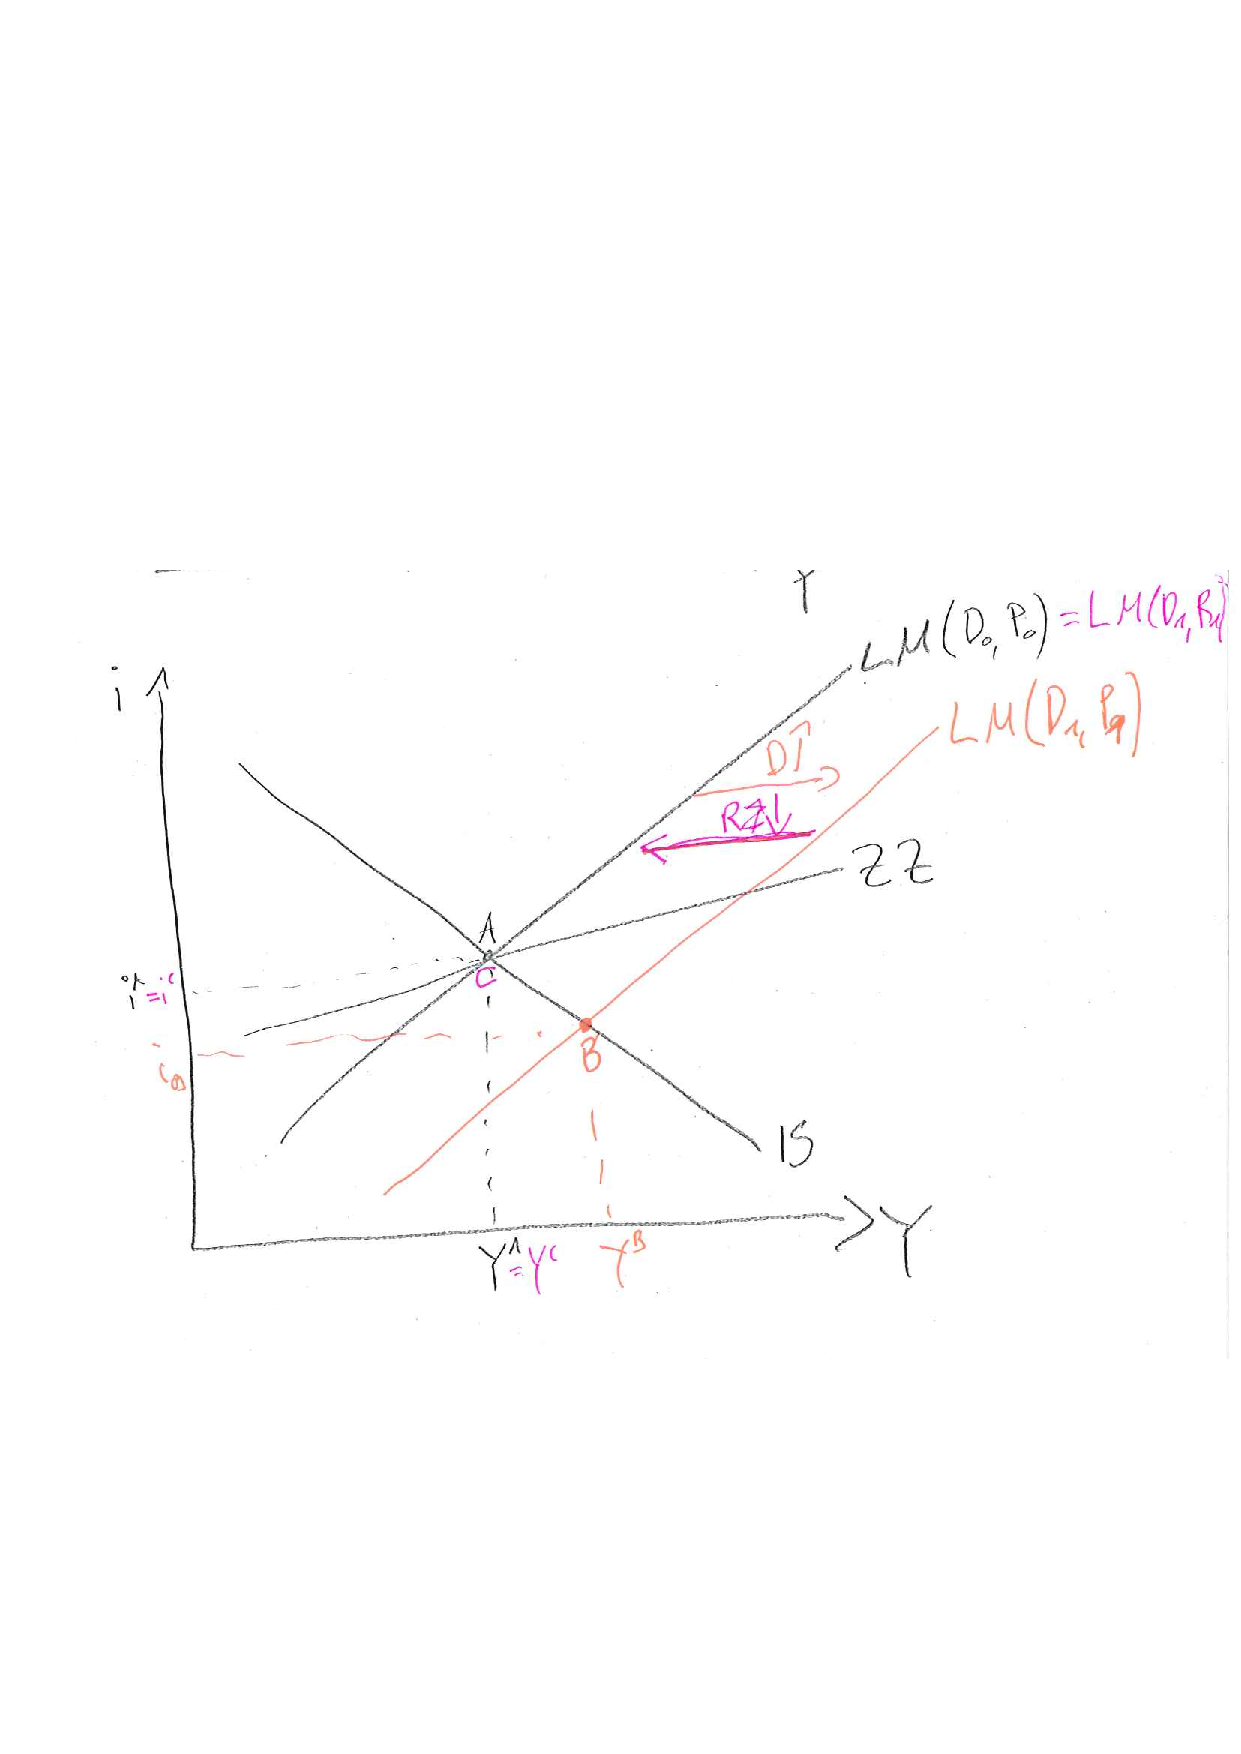
\includegraphics[width=0.5\textwidth]{Bilder/MF1.pdf}
\end{center}
  Intern.GG: $D\uparrow$, d.h. $M^s>M^d \rightarrow P_B \uparrow \rightarrow i \downarrow \rightarrow I \uparrow \rightarrow Y \uparrow$ bis $D+R = L(Y,i)$ $[A\rightarrow B ]$.
  In B gibt es eine \"{U}berschussnachfrage nach Devisen, denn:
  \begin{align*}
    \begin{rcases}
    Y \uparrow \rightarrow IM \uparrow \rightarrow LB \downarrow\\
    i \downarrow \rightarrow F\downarrow
    \end{rcases}
    \$^{N}>\$^{A}
  \end{align*}
  S m\"{u}sste steigen, heimische W\"{a}hrung m\"{u}sste abwerten. Damit S konstant bleibt, verkauft ZB Reserven $R\downarrow$, Bewegung von B zur\"{u}ck zu A bzw. C. Dies nennt man eine sterilisierte Devisenmarktintervention.

  \item Fixer WK, Hohe Kapitalmobilit\"{a}t, Expansive Fiskalpolitik, d.h. $G\uparrow$
\begin{center}
  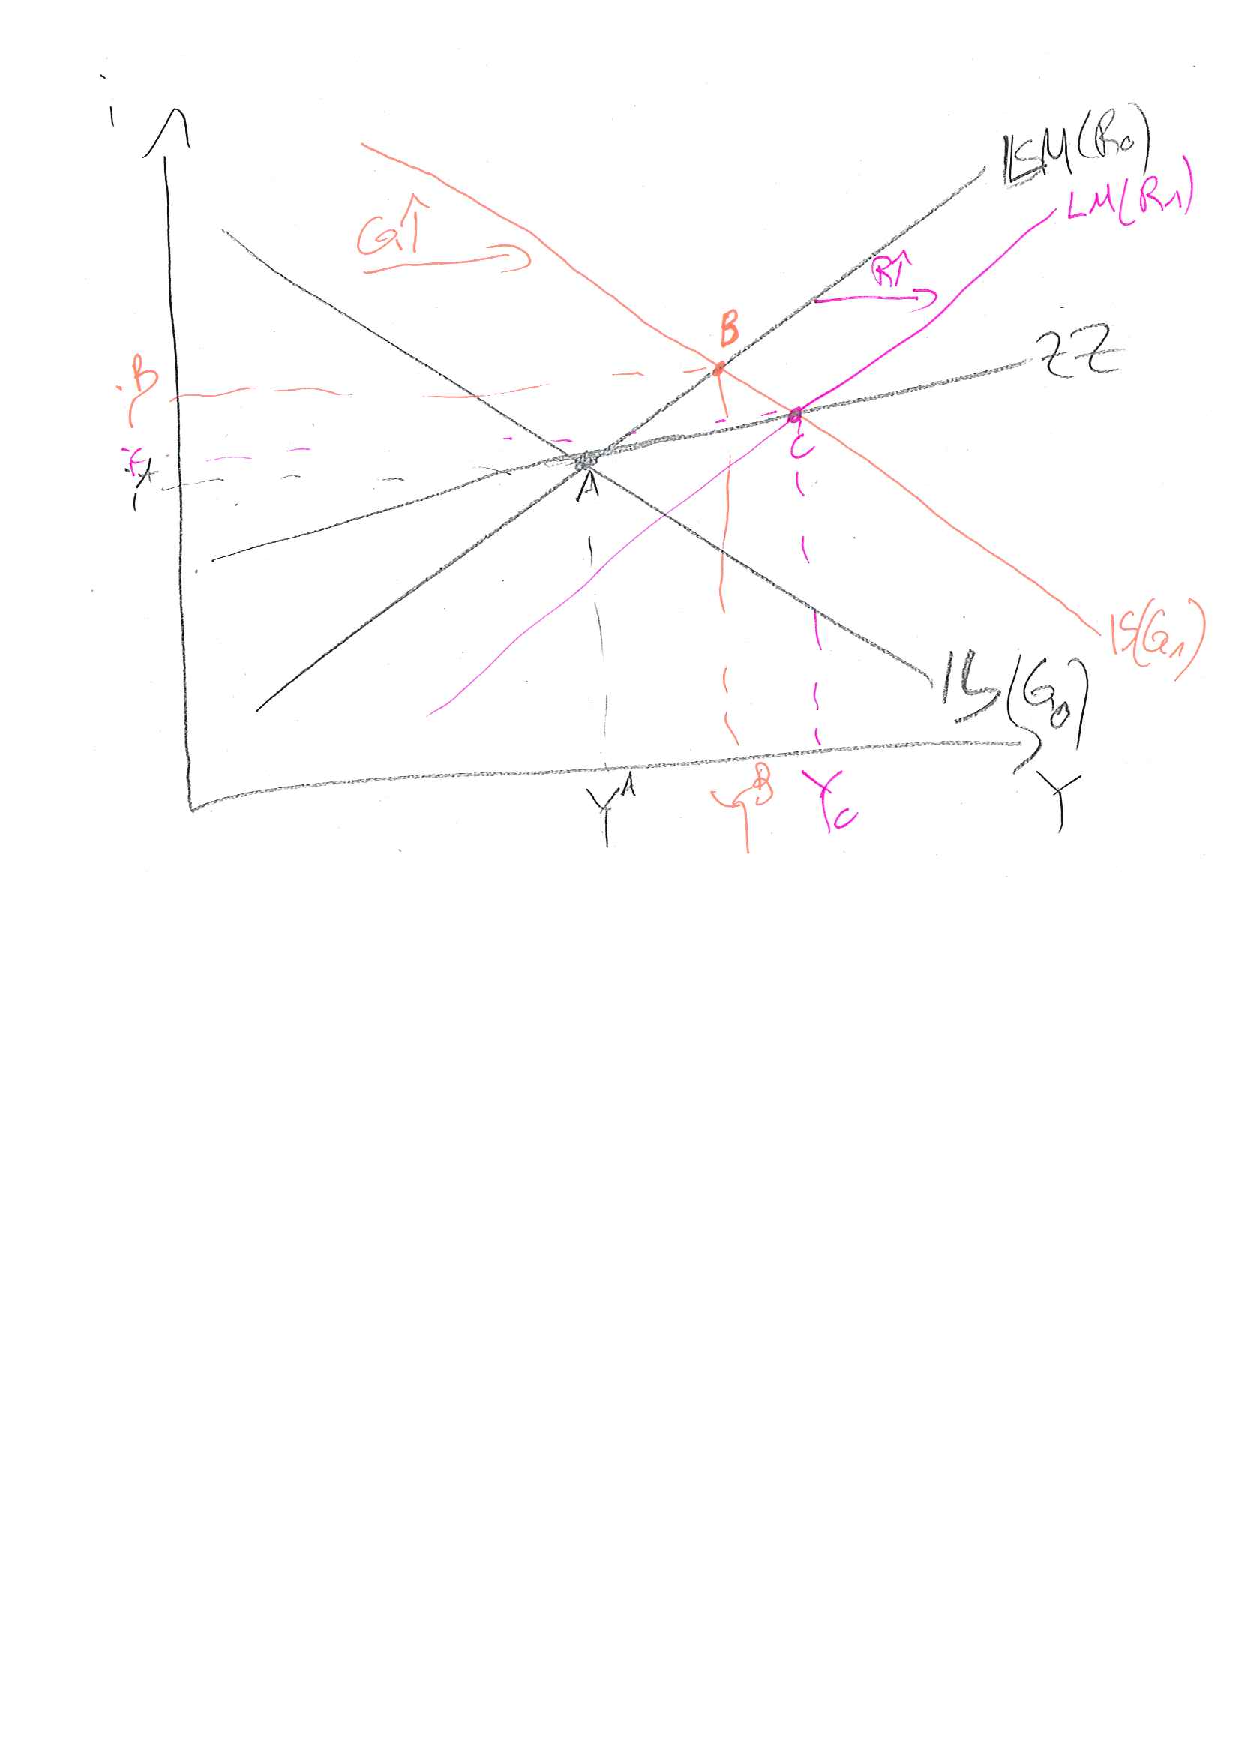
\includegraphics[width=0.5\textwidth]{Bilder/MF2.pdf}
\end{center}
  Intern.GG: $G\uparrow \rightarrow Y \uparrow$ wegen Multiplikatoreffekt, d.h. $M^d>M^s \rightarrow P_B \downarrow \rightarrow i \uparrow [A\rightarrow B ]$.
  Extern GG:
  \begin{align*}
    1:& Y\uparrow \rightarrow IM \uparrow \Rightarrow \$^{N}>\$^{A}\\
    2:& i\uparrow \rightarrow F \uparrow \Rightarrow \$^{A}>\$^{N}
  \end{align*}
  Bei hoher Kapitalmobilit\"{a}t gilt dass $2>1$, also $\$^{A}>\$^{N}$. S m\"{u}sste sinken. Damit S konstant bleibt kauft die ZB das \"{U}berschussangebot auf $\rightarrow R\uparrow \rightarrow M^{S}>M^{d} \rightarrow P_B \uparrow \rightarrow i\downarrow \rightarrow I \uparrow \rightarrow Y \uparrow [B\rightarrow C]$.
  \end{itemize}
\item Flexible WK: $S\uparrow$ d.h. Inlandsw\"{a}hrung wertet ab. Dies impliziert, dass sowohl die IS als auch die ZZ Kurven sich nach rechts verschieben (ZZ-Kurve jedoch mehr!).
\begin{itemize}
  \item Flexible WK, Hohe Kapitalmobilit\"{a}t, Expansive Geldpolitik
  \begin{center}
  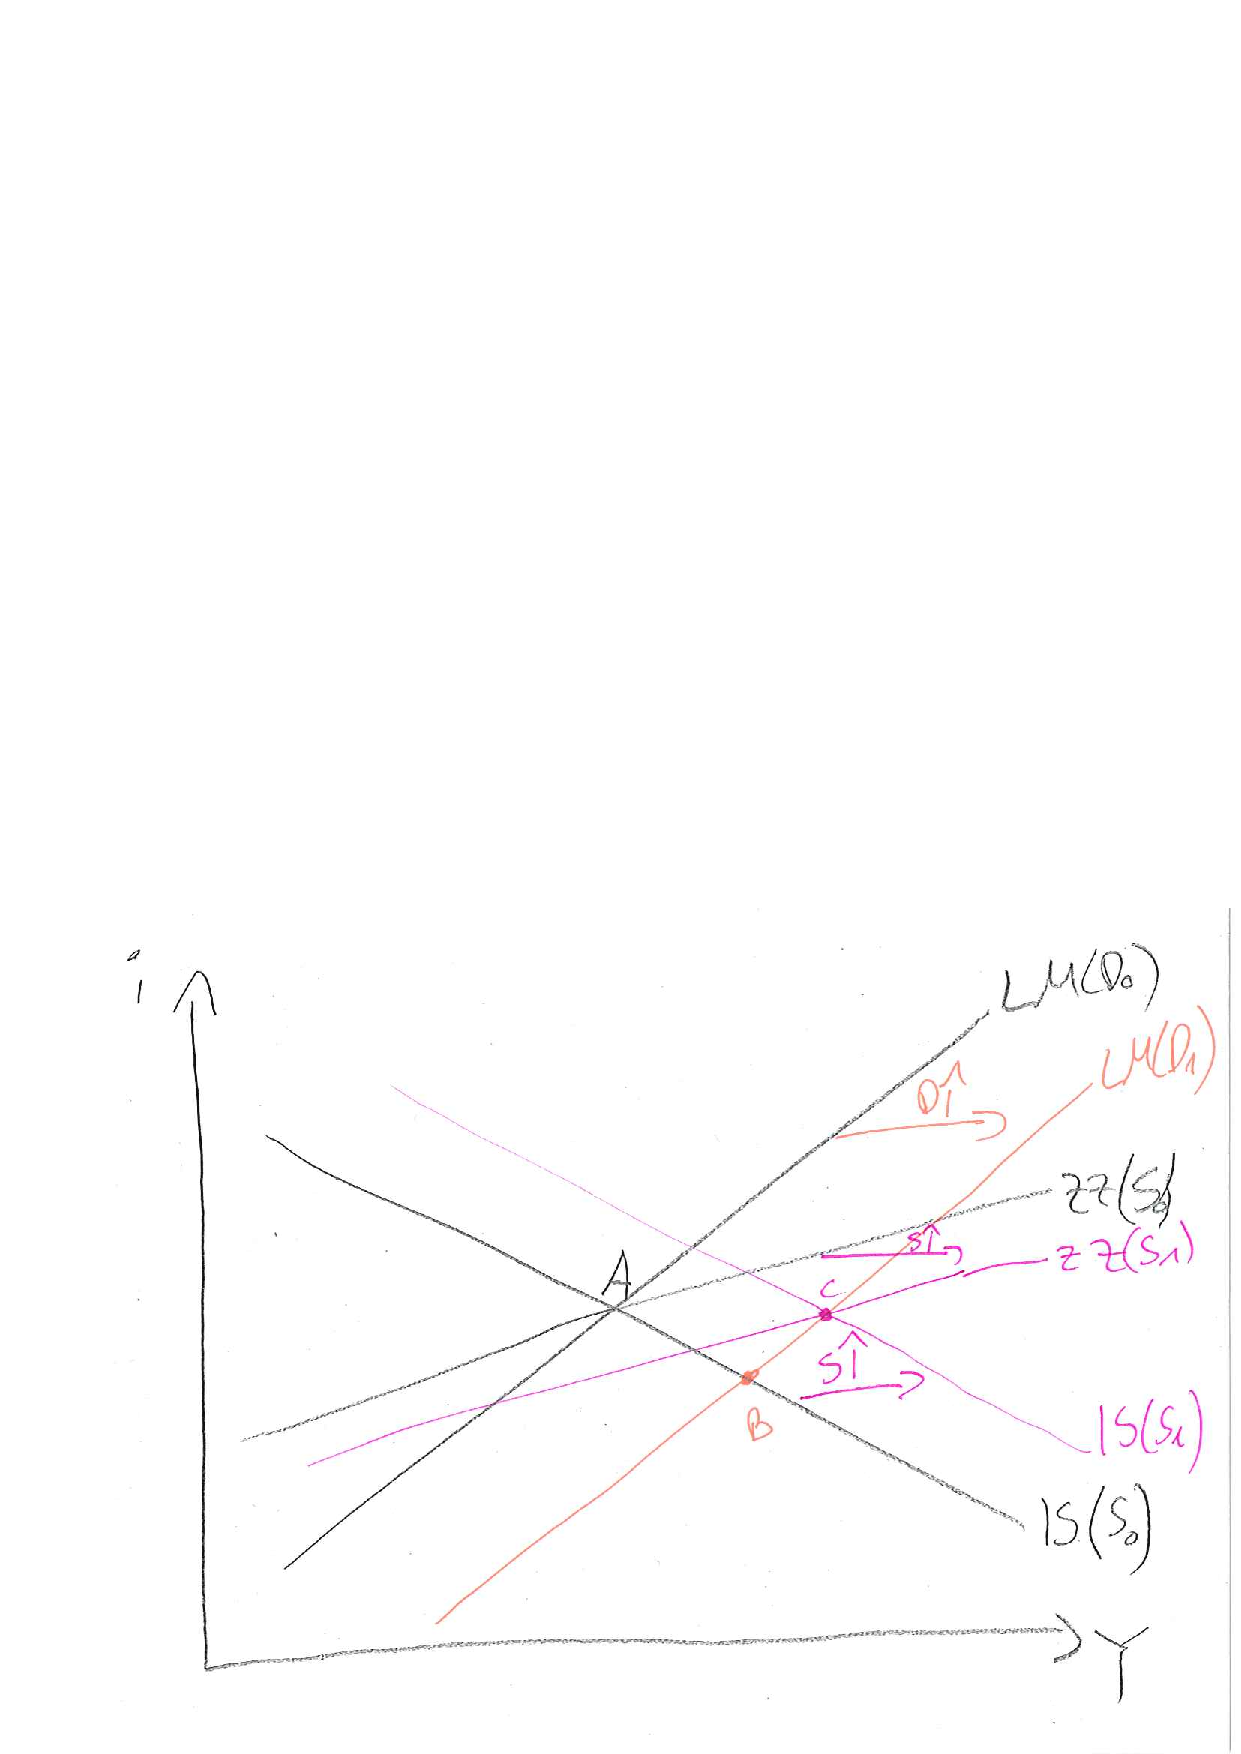
\includegraphics[width=0.5\textwidth]{Bilder/MF3.pdf}
\end{center}
    $D\uparrow \rightarrow M^s>M^d \rightarrow P_B \uparrow \rightarrow i \downarrow \rightarrow I \uparrow \rightarrow Y \uparrow [A\rightarrow B]$
    \begin{align*}
    1:& Y\uparrow \rightarrow IM \uparrow \Rightarrow \$^{N}>\$^{A}\\
    2:& i\downarrow \rightarrow F \downarrow \Rightarrow \$^{N}>\$^{A}
    \end{align*}
    Inlandw\"{a}hrung wird abgewertet, $S\uparrow$!
    \begin{align*}
      S\uparrow \rightarrow (X-IM)\uparrow \begin{cases}
        Y \uparrow \text{ (bei gegebenem i, IS nach rechts)}\\
        i \downarrow \text{ (bei gegebenem Y, ZZ nach rechts)}\\
      \end{cases}
      [B \rightarrow C]
    \end{align*}

  \item Flexible WK, Hohe Kapitalmobilit\"{a}t, Expansive Fiskalpolitik
  \begin{center}
  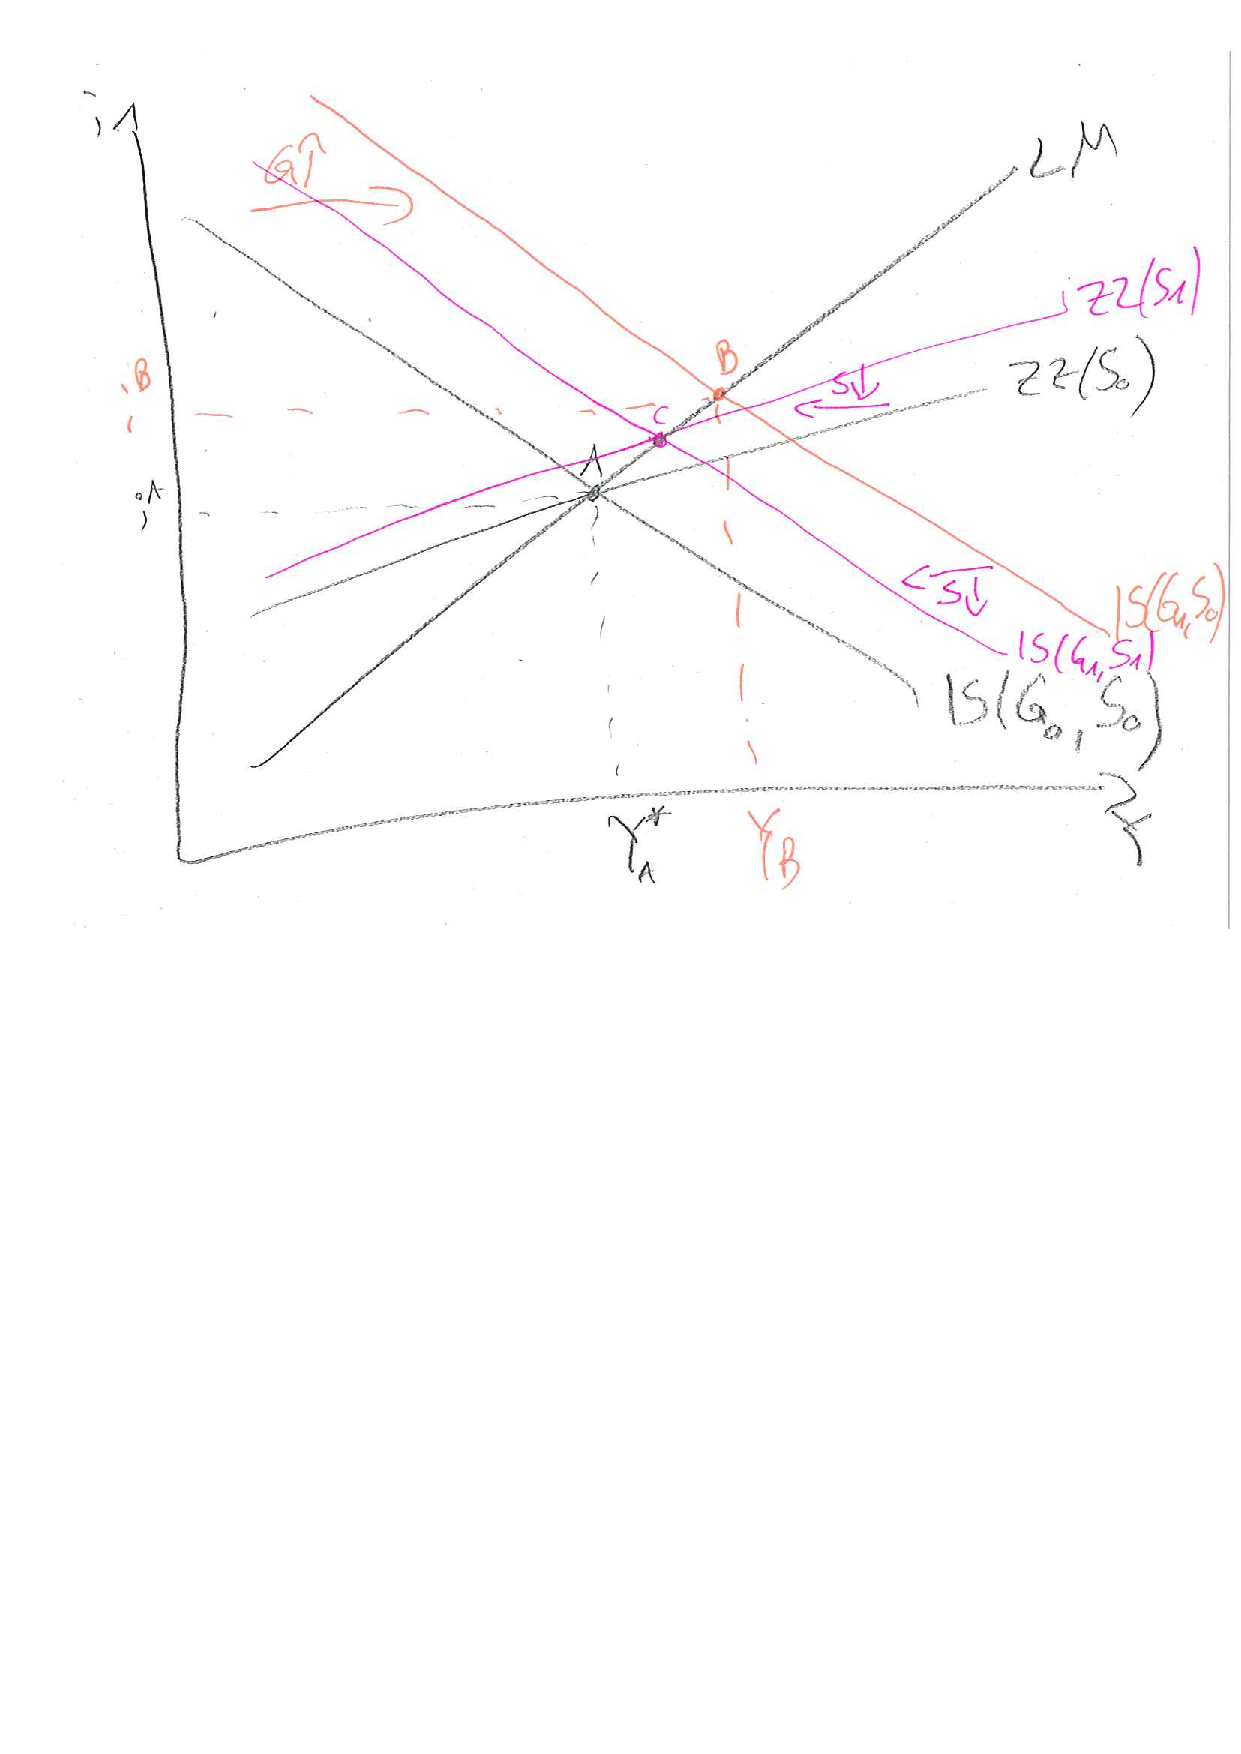
\includegraphics[width=0.5\textwidth]{Bilder/MF4.pdf}
\end{center}
$G\uparrow \rightarrow Y \uparrow \rightarrow M^d>M^s \rightarrow P_B\downarrow \rightarrow i\uparrow [A\rightarrow B]$
\begin{align*}
  \begin{rcases}
  1:& Y \uparrow \rightarrow IM \uparrow\\
  2:& i \uparrow \rightarrow F\uparrow
  \end{rcases}
  \text{Bei hoher Kap.Mobilit\"{a}t} 2>1 \rightarrow \$^{A}>\$^{N} \rightarrow S\downarrow \text{Aufwertung!}\\
  S\downarrow \rightarrow (X-IM)\downarrow
  \begin{cases}
    \rightarrow Y \downarrow \text{ IS nach links}\\
    \rightarrow i \downarrow \text{ ZZ nach links}?????
  \end{cases}
\end{align*}
\end{itemize}

\item Perfekte Kapitalmobilit\"{a}t: $i=i^* \Rightarrow$ Keine Anpassung \"{u}ber Zins m\"{o}glich! D.h., wenn es aufgrund eines \"{U}berschussangebots an Geld, eine \"{U}berschussnachfrage nach Wertpapieren gibt, wird dieses durch ein entsprechendes ausl\"{a}ndisches Angebot an Wertpapieren bei gegebenen Kursen und Zinse bedient. Ausl\"{a}ndische Wertpapiere sind in $\$$ notiert, deshalb brauchen wir Devisen, d.h. $\$^{N} > \$^{A} \rightarrow S\uparrow$.
\begin{itemize}
  \item Flexible WK, Perfekte Kap.Mobilit\"{a}t, Expansive Geldpolitik
    \begin{center}
      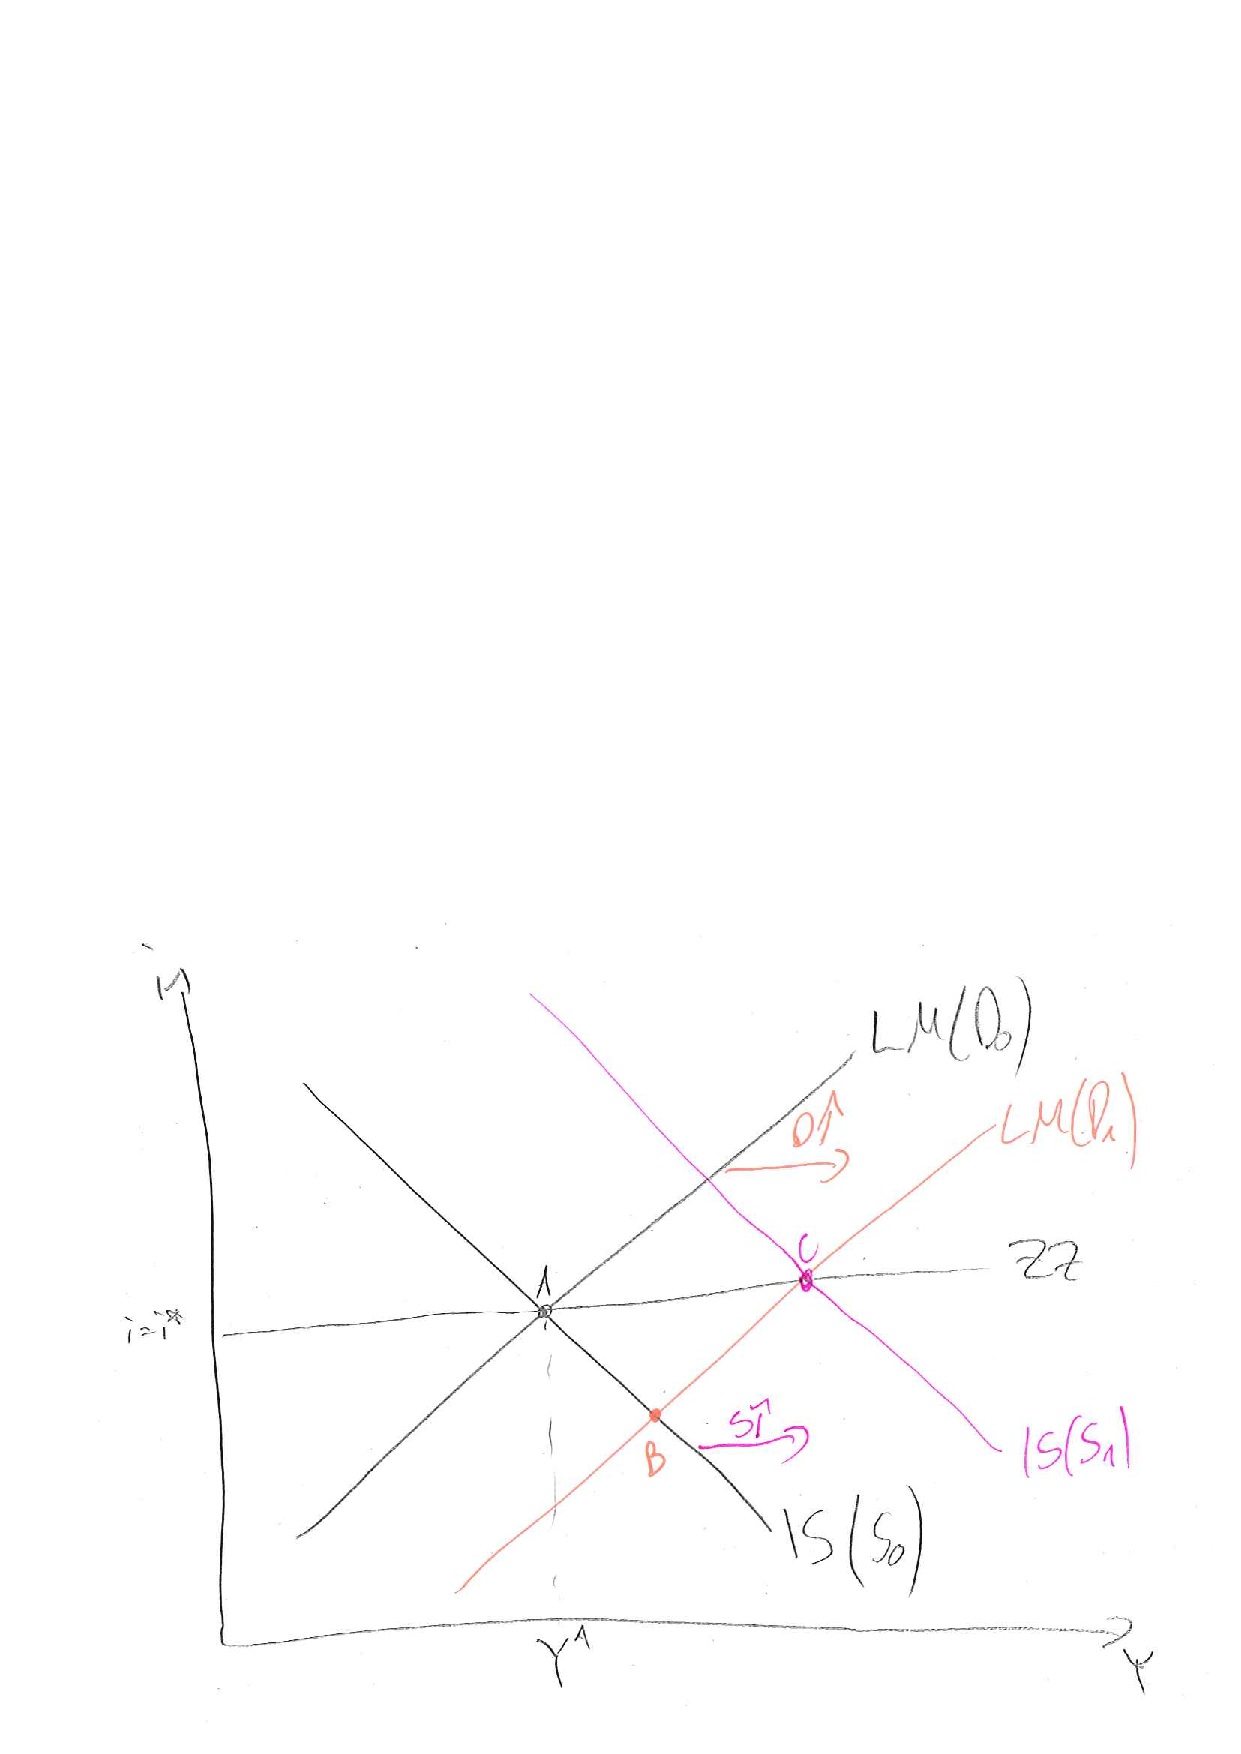
\includegraphics[width=0.5\textwidth]{Bilder/MF5.pdf}
    \end{center}
    $D\uparrow \rightarrow R+D > L$, \"{U}berschussnachfrage nach Wertpapieren, jetzt aber keine Anpassung \"{u}ber Wertpapier-Mechanismus m\"{o}glich, da $i=i^*$! $\$^{N}>\$^{A} \rightarrow $ Abwertung $S\uparrow \rightarrow (X-IM)\uparrow \rightarrow Y \uparrow [B\rightarrow C]$

\item Flexible WK, Perfekte Kap.Mobilit\"{a}t, Expansive Fiskalpolitik
    \begin{center}
      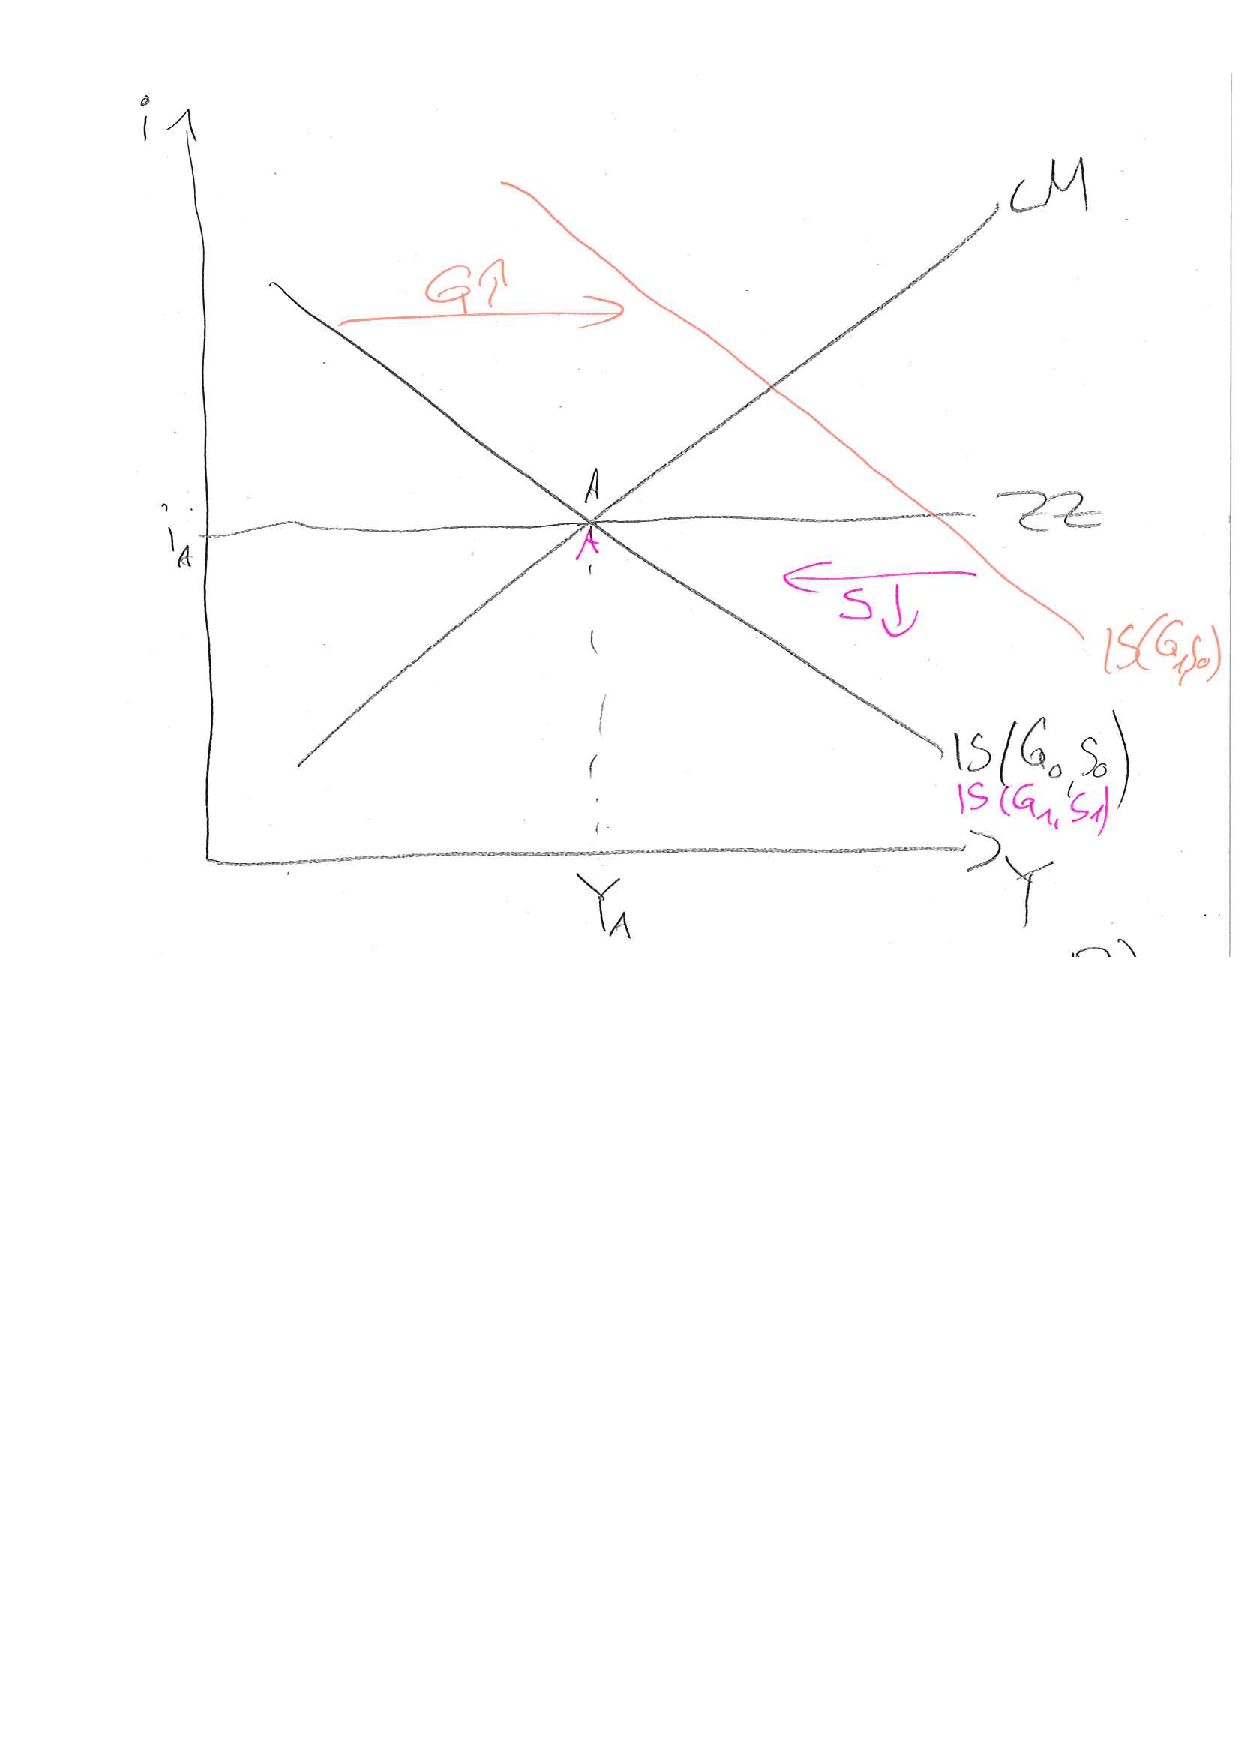
\includegraphics[width=0.5\textwidth]{Bilder/MF6.pdf}
    \end{center}
    $G\uparrow \rightarrow Y \uparrow \rightarrow L > D+R$, keine Anpassung \"{u}ber Zins m\"{o}glich, d.h. Ausland bedient Mehrangebot an Wertpapieren $\$^{A}>\$^{N} \rightarrow $ Aufwertung $S\downarrow \rightarrow (X-IM)\downarrow \rightarrow Y \downarrow [B\rightarrow A]$
\end{itemize}

\item Perfekte Kapitalmobilit\"{a}t, Konjunkturzyklus $Y^*\uparrow$
    \begin{center}
    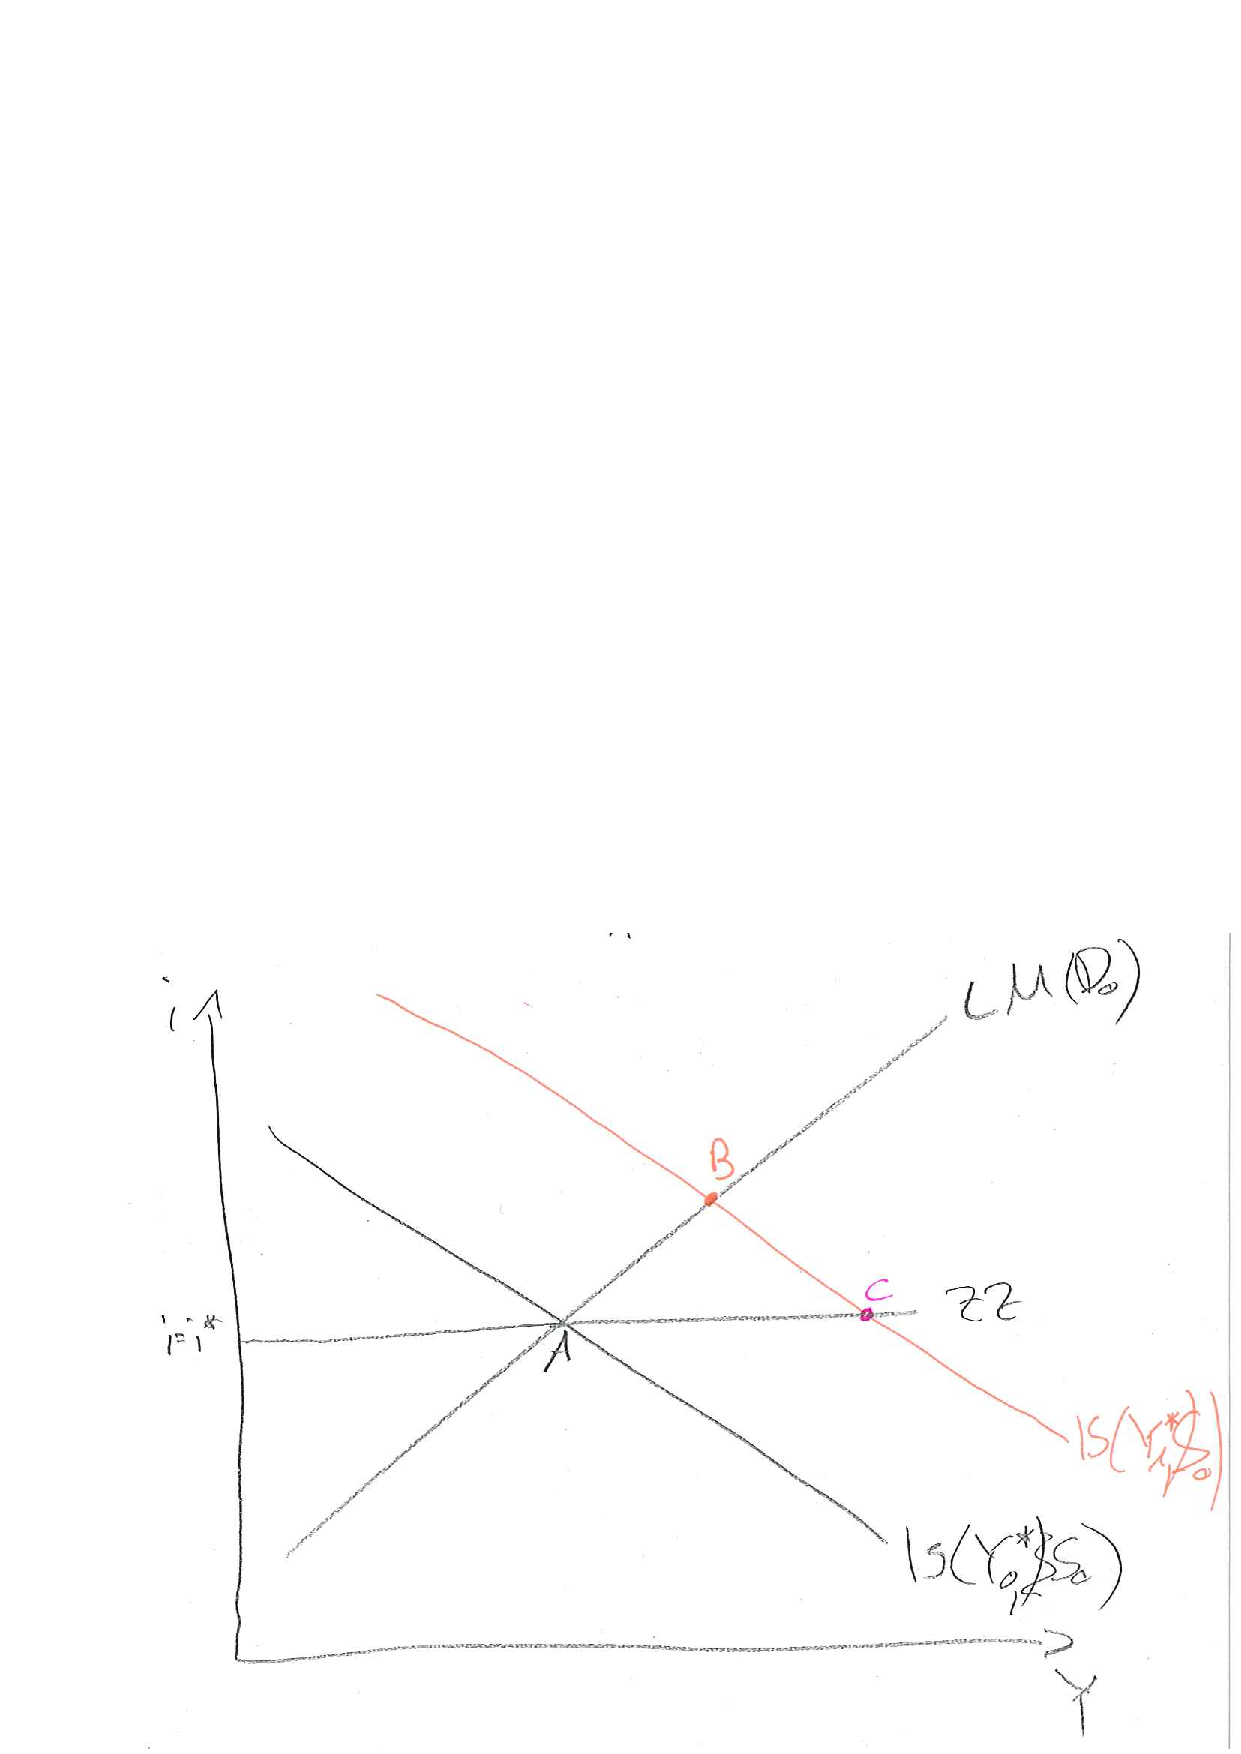
\includegraphics[width=0.5\textwidth]{Bilder/MF7.pdf}
    \end{center}
$Y^*\uparrow \rightarrow EX \uparrow \rightarrow Y \uparrow$\\
$EX \uparrow \rightarrow \$^{A}> \$^{N} [A\rightarrow B]$\\
\begin{itemize}
  \item Feste WK: ZB kauft \"{U}berangebot auf $R\uparrow$, LM nach rechts bis C! EK ist gestiegen.
  \item Flexible WK: Aufwertung $S\downarrow \rightarrow$ ausl\"{a}ndische Nachfrage wird neutralisiert! IS zur\"{u}ck zu A.
\end{itemize}
Fazit: Bei festen WK gibt es positive \"{U}bertragung, bei flexiblen WK ist die \"{O}konomie unabh\"{a}ngig vom ausl\"{a}ndischen Konjunkturverlauf!
\end{enumerate}


\section{Arbeitsmarkt und AS-AD Modell}
\subsection{Arbeitsmarkt und Aggregierte Angebot}
\begin{enumerate}[a)]
  \item \begin{itemize}
    \item Lohnsetzung: $W=P^e F(\overset{-}{u},\overset{+}{z})$.
    \begin{itemize}
    \item F\"{u}r Lohnsetzung ist erwarteter Reallohn,$W/P^e$, entscheidend, denn dies ist die Kaufkraft der Arbeitnehmer. In Vertr\"{a}gen werden jedoch Nominall\"{o}hne festgelegt, dabei st\"{u}tzt man sich auf das erwartete Preisniveau, da das tats\"{a}chliche noch nicht bekannt ist.
    \item Arbeitslosenquote $u = \frac{U}{L^s}, u\uparrow \rightarrow \frac{W}{P^e}\downarrow$, da Verhandlungsmacht der AN sinkt und die der AG steigt, d.h. $\frac{\partial F}{\partial u}<0$. Zu Verhandlungsmacht z\"{a}hlen \"{U}berlegungen: wie ersetzbar ist ein Arbeiter? Wie schnell findet ein Arbeiter einen neuen Job. Wenn u klein ist, Unternehmen finden schwer Ersatz, Arbeiter jedoch finden leichter einen Job, haben also mehr Verhandlungsmacht.
    \item Sammelvariable z: Per Annahme positiver Einfluss, z.B. Reservationslohn, Effizienzlohn, Arbeitslosenversicherung, Mindestlohn, K\"{u}ndigungsschutz. Im Allgemeinen ist dies der Grad der Arbeitsmarktfriktionen
  \end{itemize}
  \item Preissetzung: Zuschlagskalkulation: $\mu$ ist Lohnkostenzuschlag. Bei vollkommenen Wettbewerb w\"{a}re P=GK=W und somit $\mu=0$.
  \end{itemize}
  \item $L^S = U + N, u = \frac{U}{L^s} \Leftrightarrow U = u L^s \Rightarrow N = L^s - U = L^s - uL^s = (1-u)L^s$. Also $u=1 - \frac{N}{L^s}.$\\
  Es gilt $P=P^e$. Somit k\"{o}nnen wir die nat\"{u}rliche Arbeitslosigkeit, die nat\"{u}rliche Besch\"{a}ftigung und die nat\"{u}rliche Produktion berechnen!
  \begin{align*}
    \frac{W}{P^e} = \frac{W}{P} = F(u,z) = F\left(1 - \frac{N}{L^s},z\right) (WS)\\
    \frac{W}{P} = \frac{1}{1+\mu} (PS)
  \end{align*}
\begin{center}
  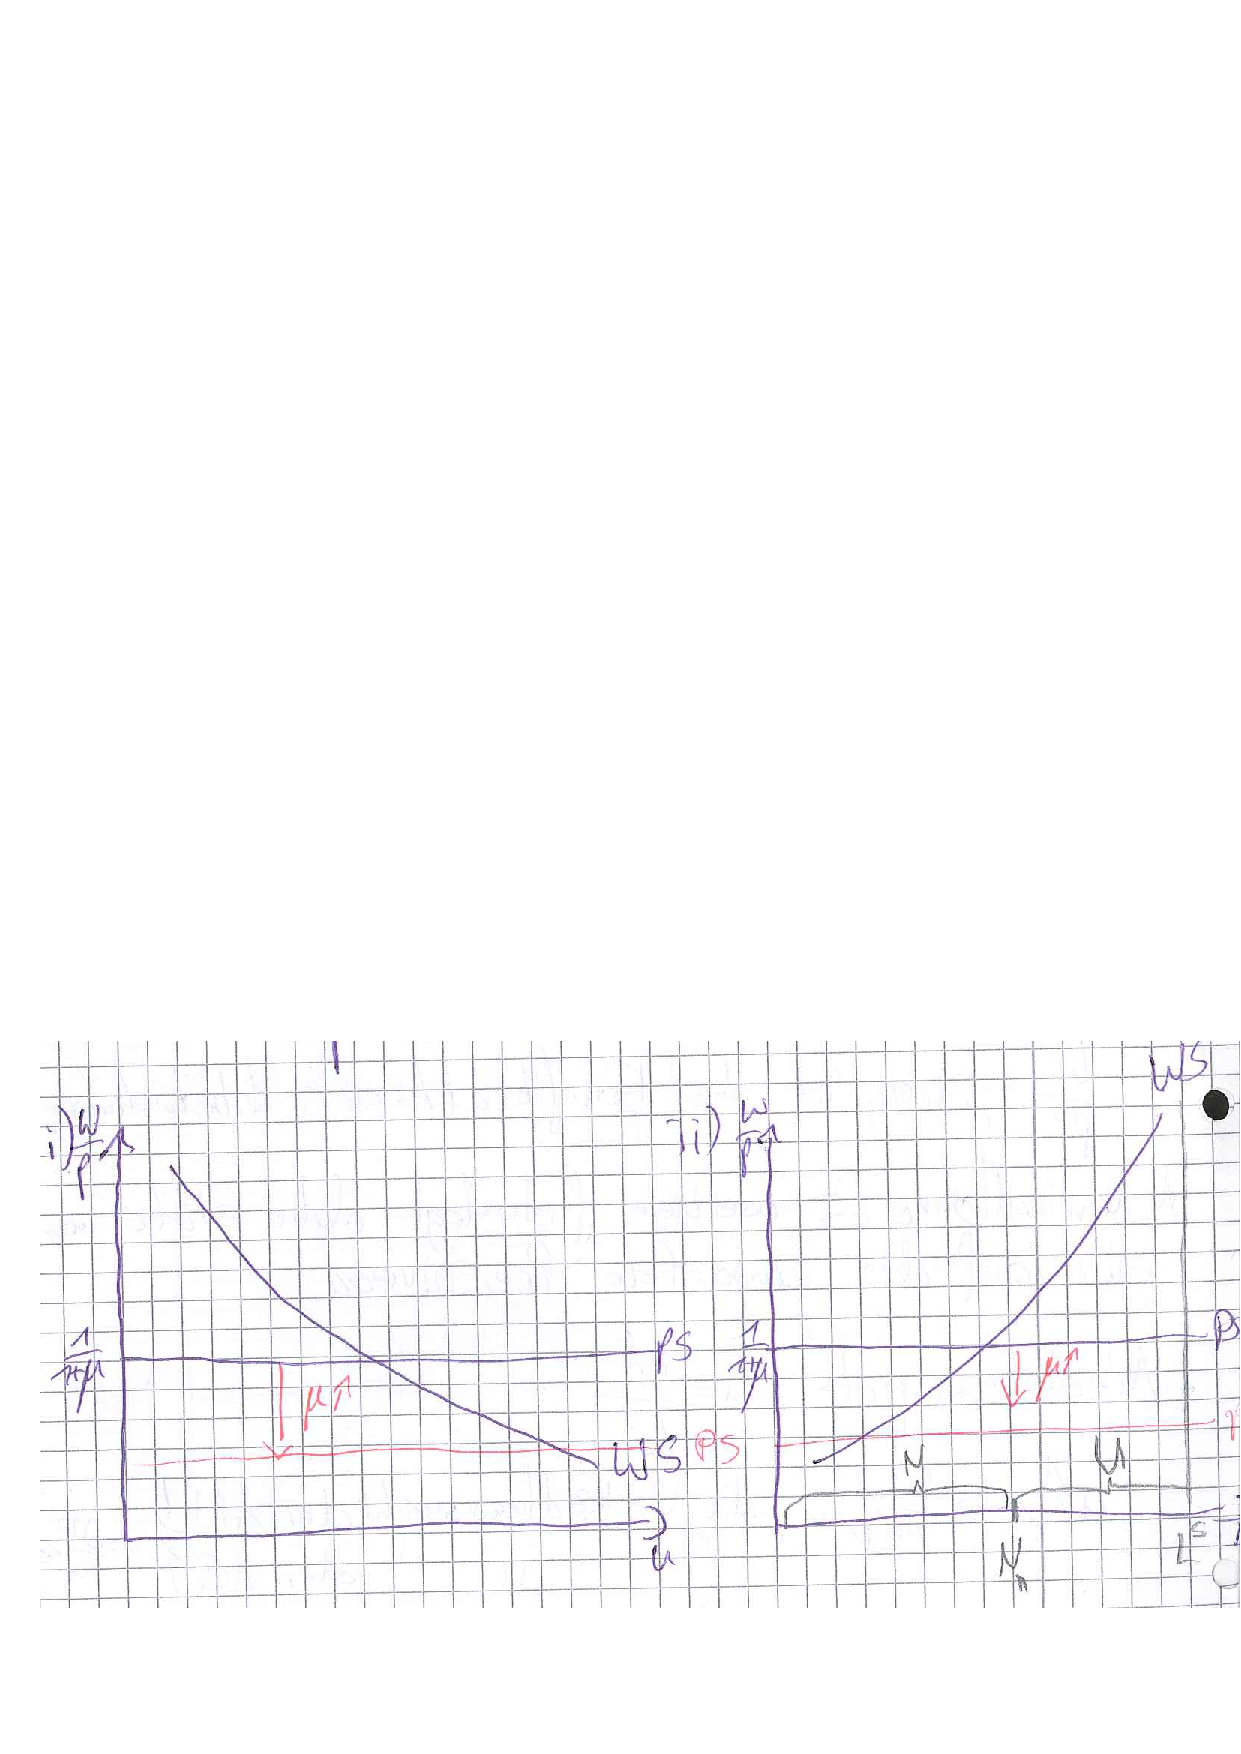
\includegraphics[width=0.8\textwidth]{Bilder/WSPSDiagramm.pdf}
\end{center}
  Interpretation: AN bilden Lohnforderungen auf Basis des aktuellen erwarteten Preisniveaus unabh\"{a}ngig von der Preissetzung der Unternehmen. Im GG ist Reallohn gleich dem Lohn, den die Unternehmen bereit sind zu zahlen und den Forderungen der AN f\"{u}r das aktuelle erwartete bzw. beobachtete Preisniveau. $P=P^e$ beschreibt die mittlere Frist, denn Preiserwartungen erf\"{u}llen sich! Wenn $P=P^e$ eintritt, dann ergibt sich die sogenannte strukturelle oder nat\"{u}rliche Besch\"{a}ftigung, Arbeitslosigkeit und Produktion. Determinanten davon sind $\mu$ und z!
  \begin{itemize}
    \item $z\uparrow \rightarrow \frac{W}{P}\uparrow \rightarrow N^{d} \downarrow \rightarrow u \uparrow \Rightarrow \frac{W}{P} \downarrow$ (WS) verschiebt sich nach oben!
    \item $\mu \uparrow \rightarrow \frac{W}{P} \downarrow \rightarrow N^s \downarrow \rightarrow u \uparrow$ (PS) verschiebt sich nach unten! $\mu$ ist Ma{\ss} f\"{u}r Wettberwerbsintensit\"{a}t ($\mu=0$ perfekter Wettbewerb)
  \end{itemize}
  \item Jetzt: K\"{u}rzere Frist, da $P^e \neq P$, bzw. konstante Preiserwartungen!\\
  Idee: AS-Kurve kombiniert Preis- und Lohnsetzungsgleichung, sie gibt Zusammenhang zwischen P und Y f\"{u}r gegebene Preiserwartungen $P^e$ wieder.\\
  Herleitung: Einsetzen von $Y=\underbrace{A}_{=1}N = N$ und (WS) in (PS)
  \begin{align*}
    W = \frac{P}{1+\mu}\\
    W = P^e z\underbrace{(1-u)L}_{N} = P^e z N = P^e z Y\\
    \Rightarrow P =(1+\mu)P^e z Y
  \end{align*}
  Steigung: $\frac{\partial P}{\partial Y} = (1+\mu) P^e z > 0$. Interpretation: Mit h\"{o}herem Output steigt Besch\"{a}ftigung bzw. Arbeitslosigkeit sinkt. Dies f\"{u}hrt zu besserer Verhandlungsmacht der AN, somit zu h\"{o}heren L\"{o}hnen. H\"{o}here L\"{o}hne bedeutet, h\"{o}here Kosten und somit h\"{o}here Preise! (Bewegung auf der AS Kurve)\\
  Lage: Erh\"{o}hung von Preiserwartungen: F\"{u}r jedes Outputniveau f\"{u}hren h\"{o}here Preiserwartungen zu h\"{o}heren Lohnforderungen, und damit letztlich zu h\"{o}heren Preisen. (Verschiebung der AS nach oben)
  \begin{center}
  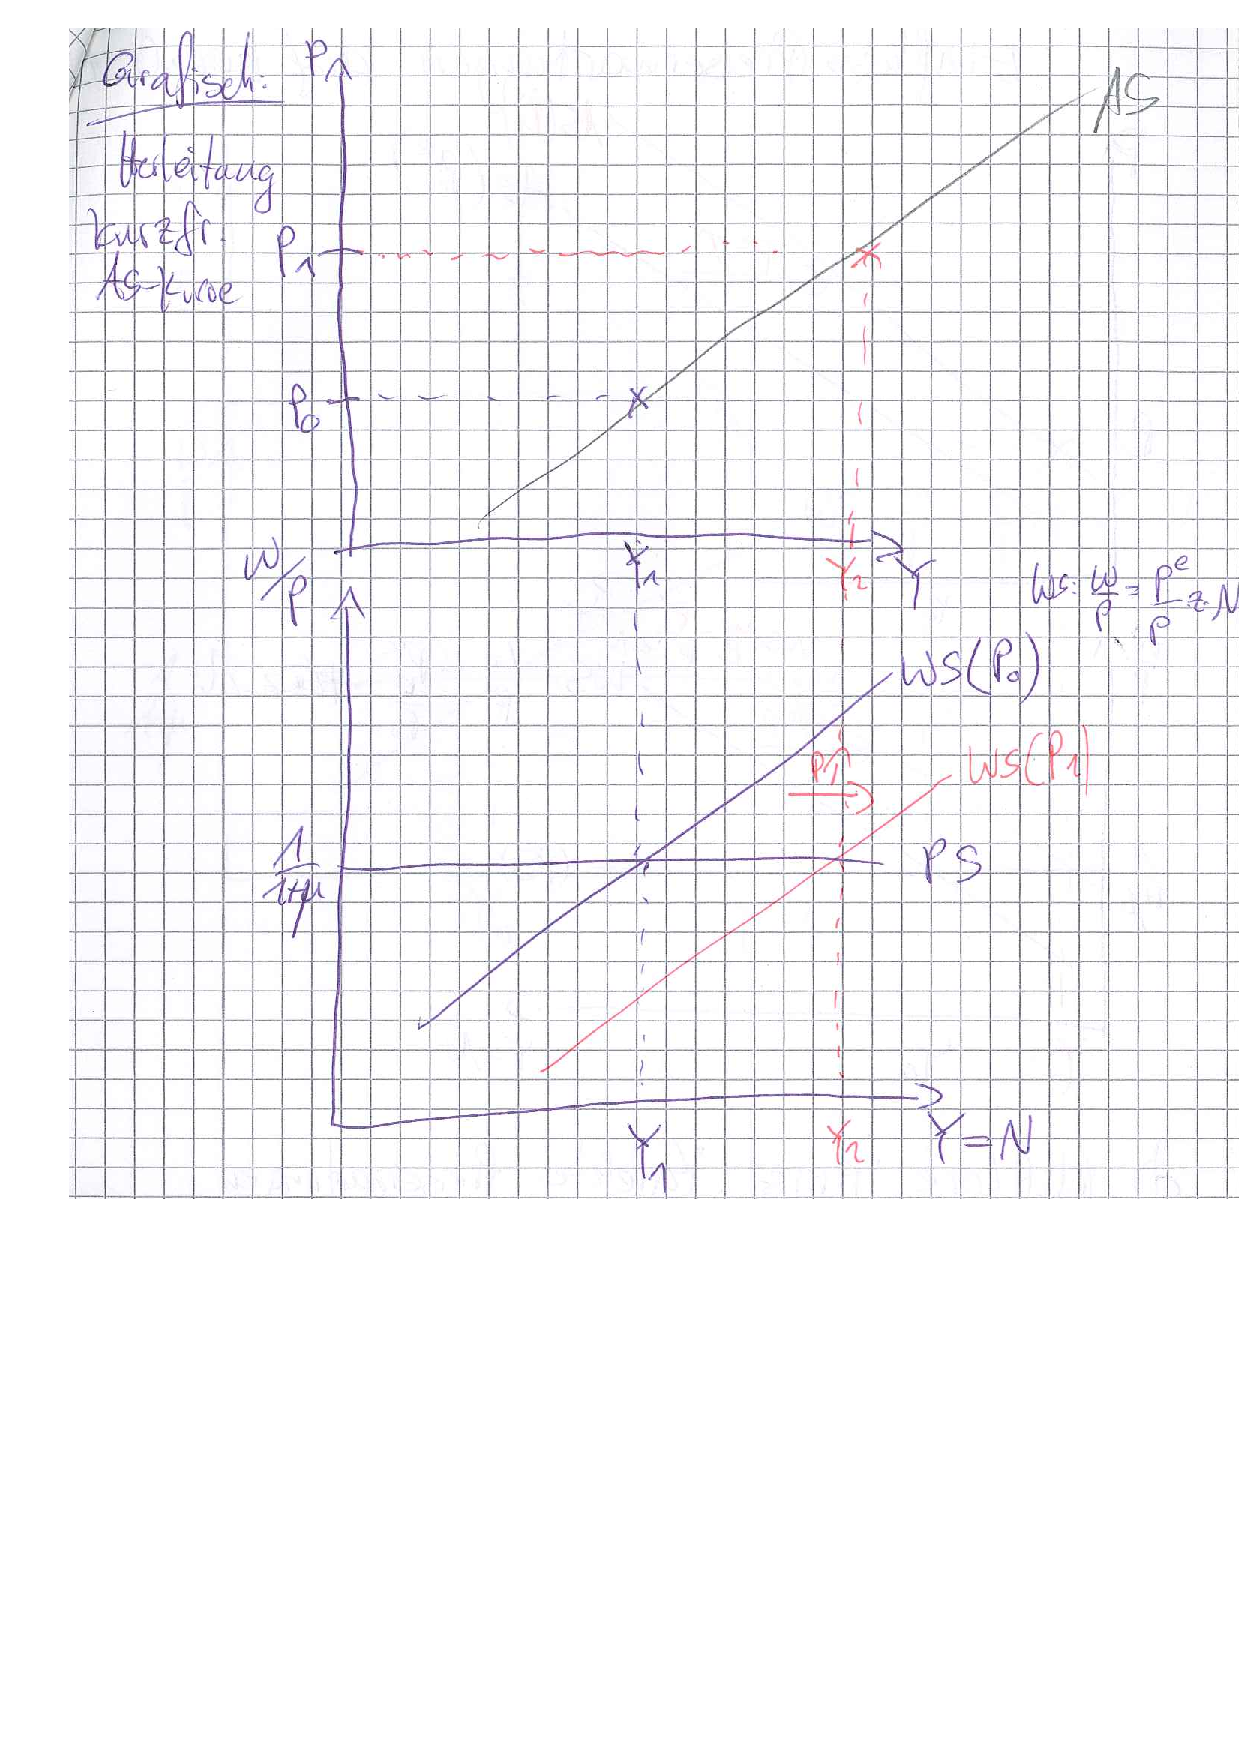
\includegraphics[width=\textwidth]{Bilder/ASkurzeFrist.pdf}
\end{center}
Einfluss von Preiserwartungen auf kurzfristige AS
  \begin{center}
  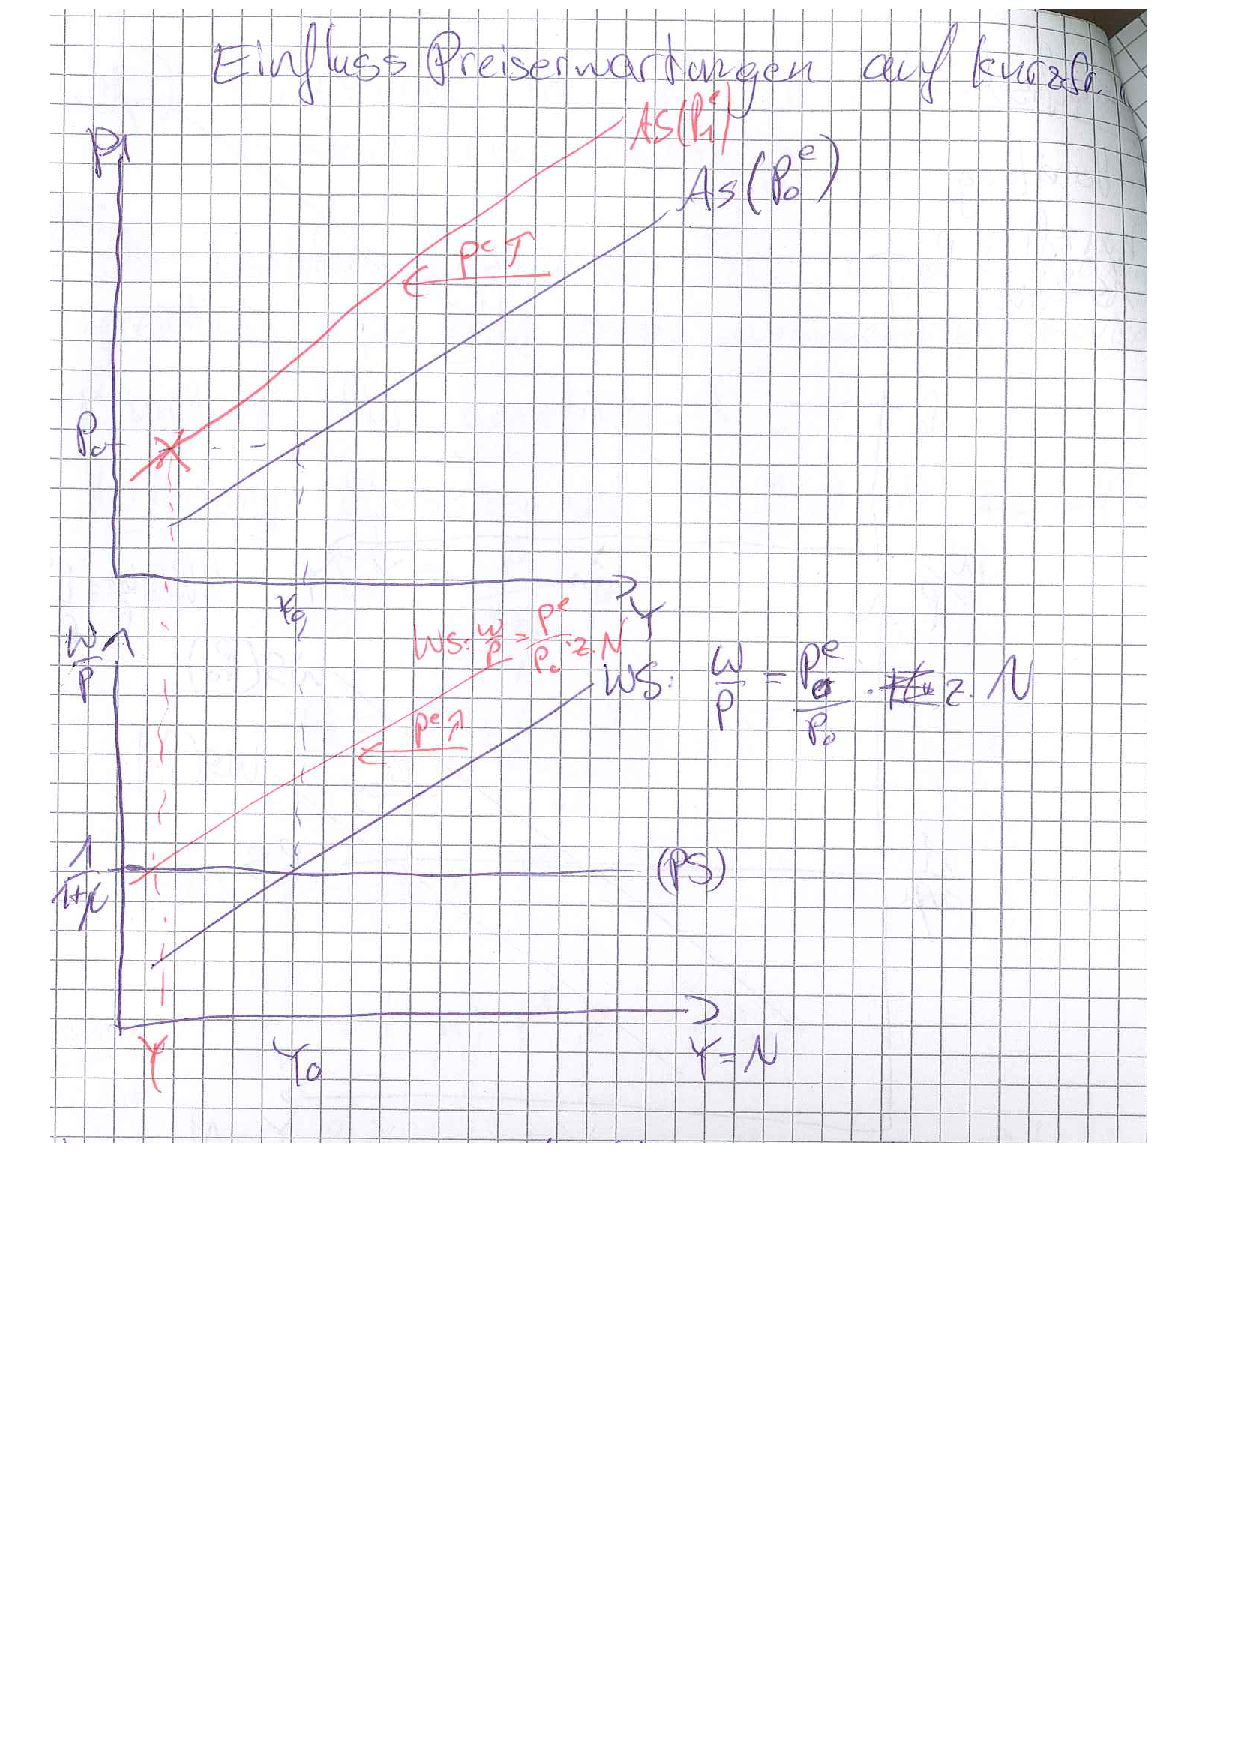
\includegraphics[width=\textwidth]{Bilder/ASkurzeFristPe.pdf}
\end{center}
\item Mittlere Frist: Korrekte Preiserwartungen, wir k\"{o}nnen nat\"{u}rliche Gr\"{o}{\ss}en berechnen. AS-Kurve verl\"{a}uft vertikal, also unabh\"{a}ngig vom Preisniveau $P=P^e$. Interpretation: Arbeitsmarkt im GG, Produktion und Besch\"{a}ftigung auf ihrem strukturellem Niveau!
      \begin{center}
  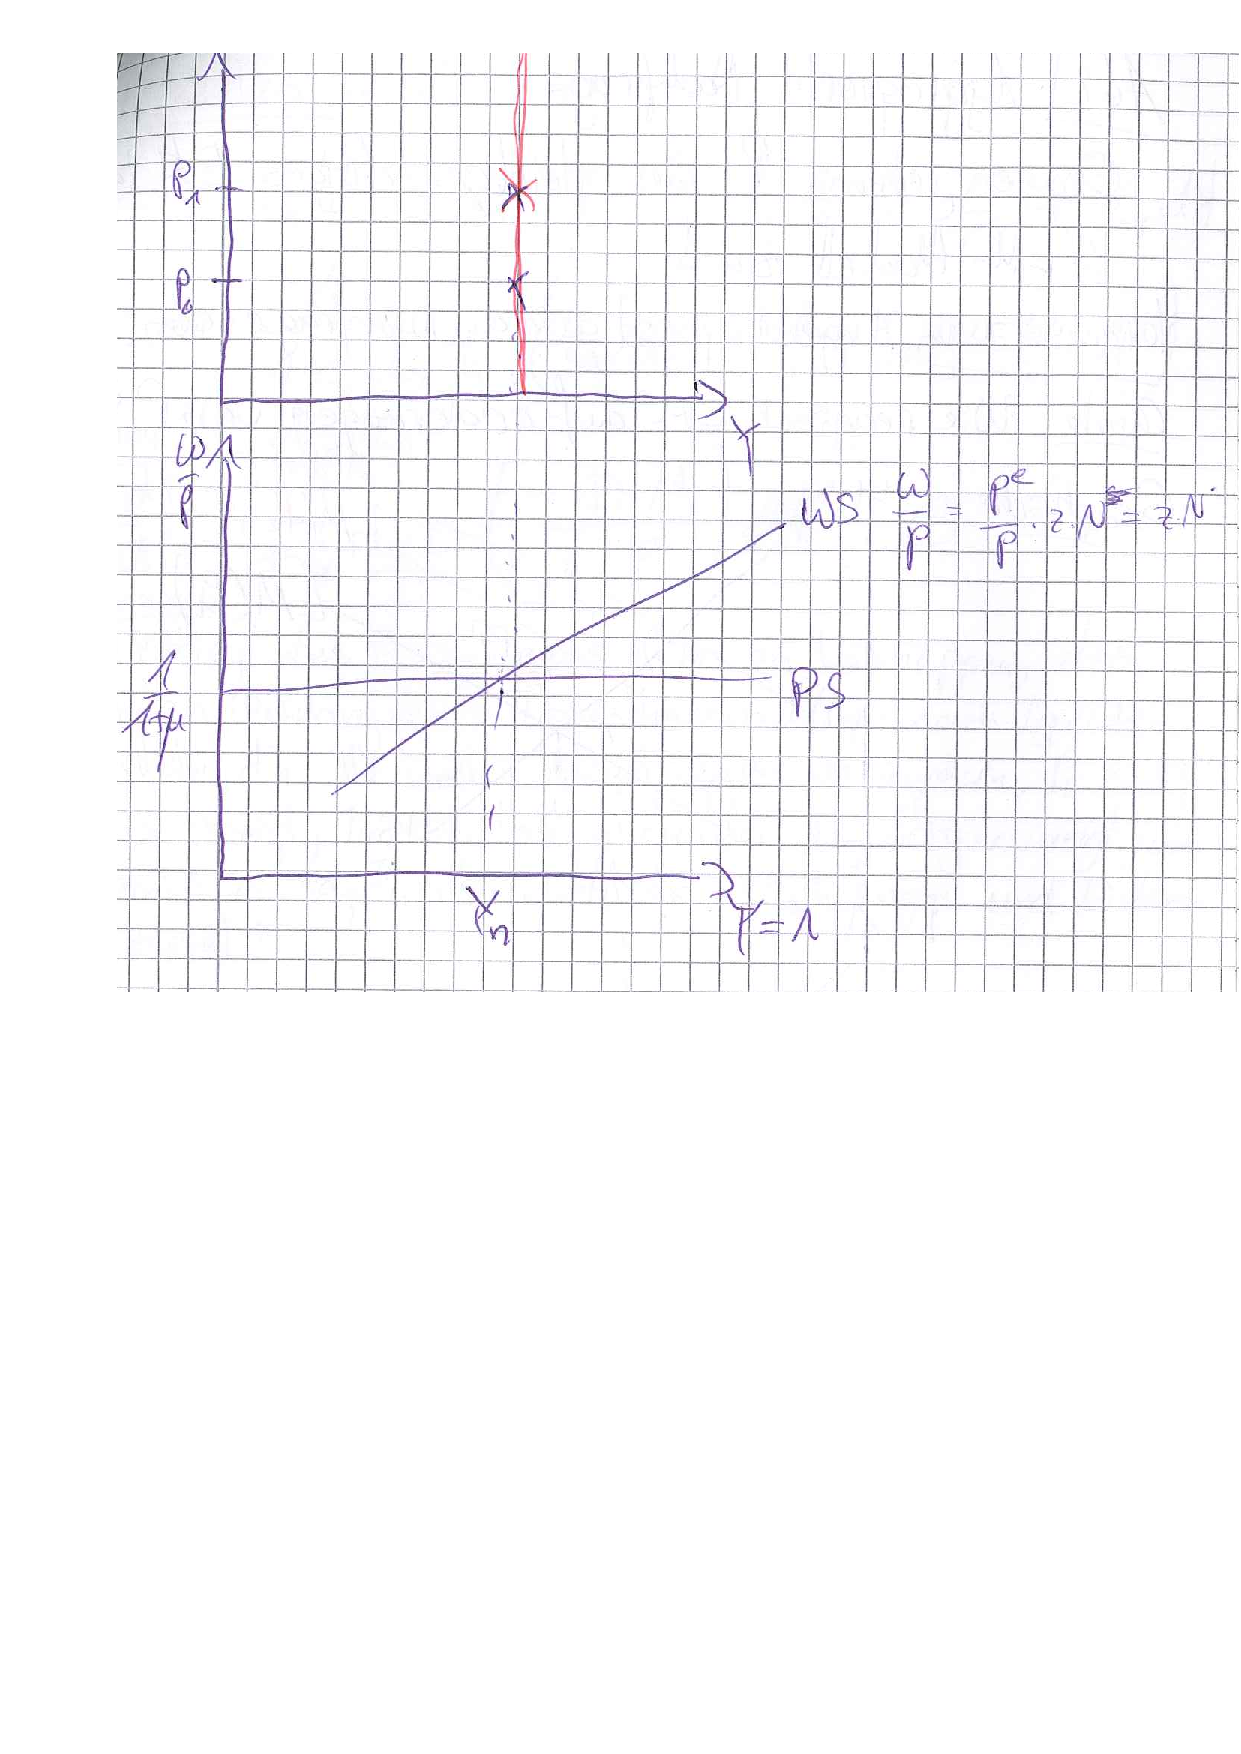
\includegraphics[width=\textwidth]{Bilder/ASmittlereFrist.pdf}
\end{center}
Anpassung findet statt, da Preiserwartungen sich anpassen!
      \begin{center}
  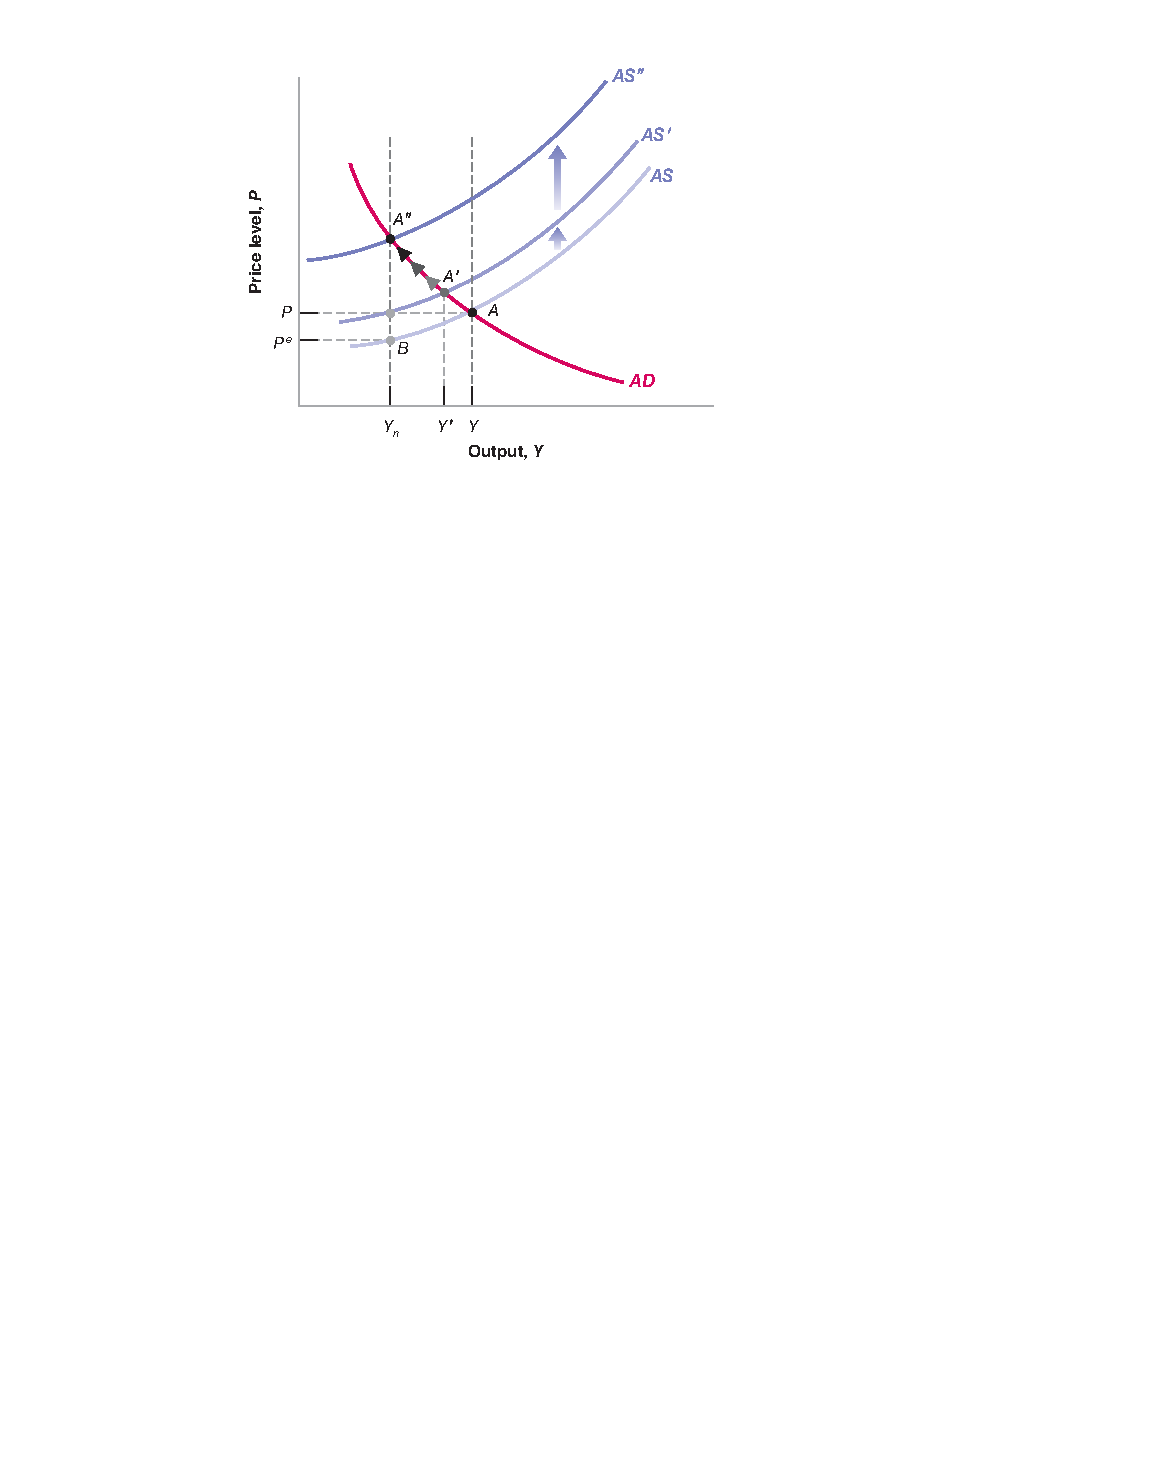
\includegraphics[width=0.6\textwidth]{Bilder/ASmittlereFristAnpassung.pdf}
\end{center}
\end{enumerate}

\subsection{Aggregierte Nachfrage (AD-Modell)}
\begin{enumerate}[a)]
  \item Aggregierte Nachfragefunktion: Ordnet jedem p ein gleichgewichtiges Einkommen im IS-LM-Modell zu. Voraussetzung also: Angebot passt sich an Nachfrage an. Grob: Wie reagiert LM auf \"{A}nderungen von P?\\
  $P \uparrow \rightarrow L > \frac{M}{P} \rightarrow P_B \downarrow \rightarrow i \uparrow \rightarrow I \downarrow \rightarrow Y \downarrow$\\
  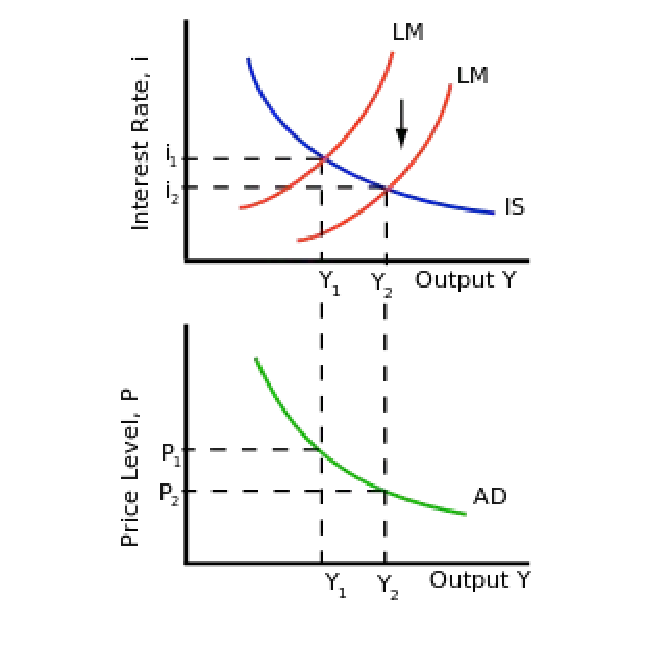
\includegraphics[width=0.5\textwidth]{Bilder/ADHerleitung.pdf}
  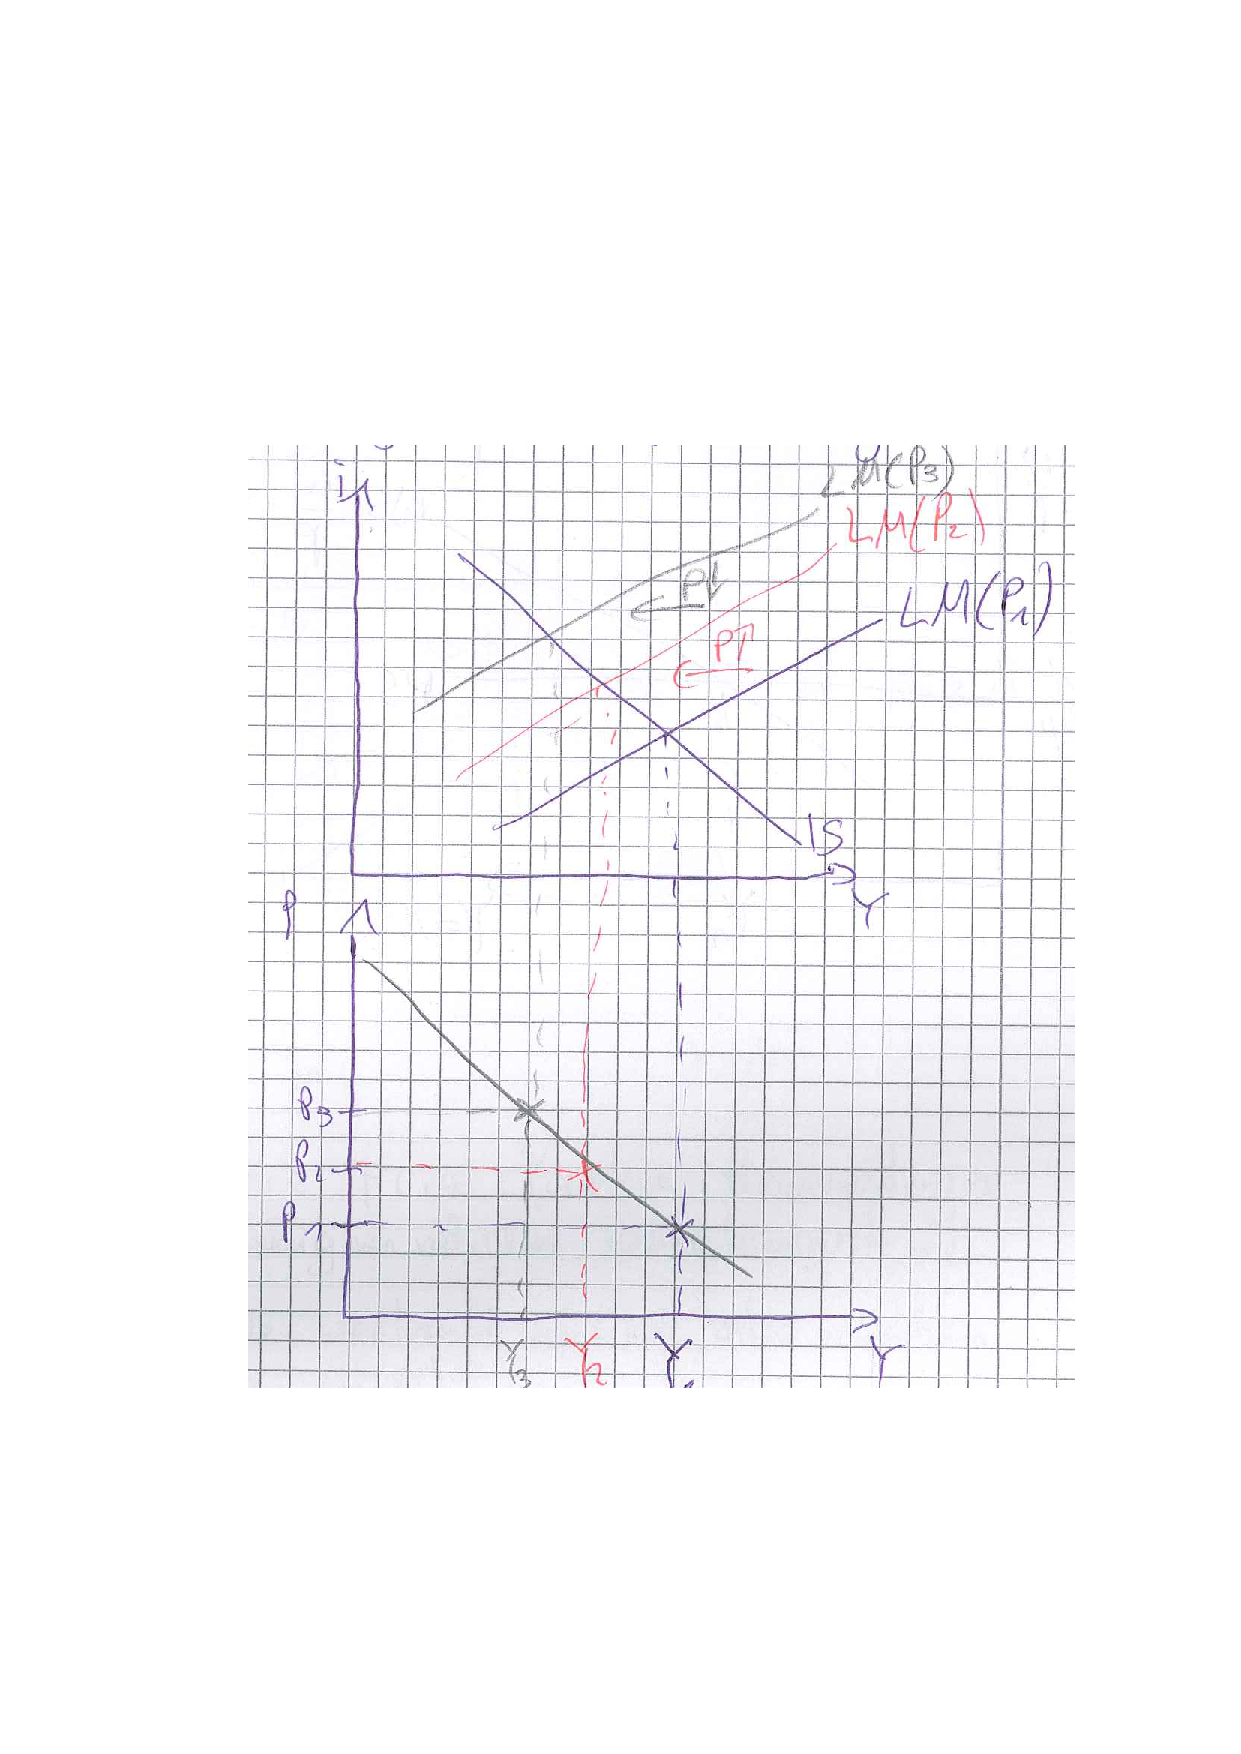
\includegraphics[width=0.5\textwidth]{Bilder/ADHerleitung2.pdf}
  Analytisch: LM nach i umformen und in IS einsetzen, ergibt:
  \begin{align*}
     Y &= \frac{1}{1-c -\frac{b L_Y}{L_i}} \left(C_{aut} - c T_{aut} + I_{aut} +G_{aut} - \frac{b}{L_i}\frac{M}{P}\right)\\
     dY &= \frac{1}{1-c -\frac{b L_Y}{L_i}} \left(dC_{aut} - c dT_{aut} + dI_{aut} +dG_{aut} - \frac{b}{L_i} \left(\frac{1}{P}dM-\frac{M}{P^2}dP\right)\right)\\
     \frac{dY}{dP} &= \frac{1}{1-c -\frac{b L_Y}{L_i}} \left(\frac{b}{L_i}\frac{M}{P^2}\right) <0
  \end{align*}
  Anstieg des Preisniveaus f\"{u}hrt zu Verknappung des realen Geldangebots. \"{U}berschussnachfrage nach liquiden Mitteln: HH wollen Wertpapiere ver\"{a}{\ss}ern, $P_B$ sinkt, Zins steigt, Investitionen werden zur\"{u}ckgedr\"{a}ngt und somit gesamtwirtschaftliche Nachfrage und Einkommen gesenkt.\\
  AD ist GG-Kurve und keine mikro\"{o}konomische Verhaltensbeziehung!\\
  \item Zinssatz\"{a}nderung:\\
  Entspricht der Frage nach dem Einfluss des Zinses auf das Einkommen im IS-LM-Modell
  \begin{itemize}
    \item Zins ist aber endogen!
    \item Jedem Punkt auf der AD-Kurve entspricht ein GG-Zins
    \item Einfluss also nicht feststellbar!
  \end{itemize}

  \item Lage der AD-Kurve:
  \begin{enumerate}
    \item $dG >0$ oder $dT<0$\\
      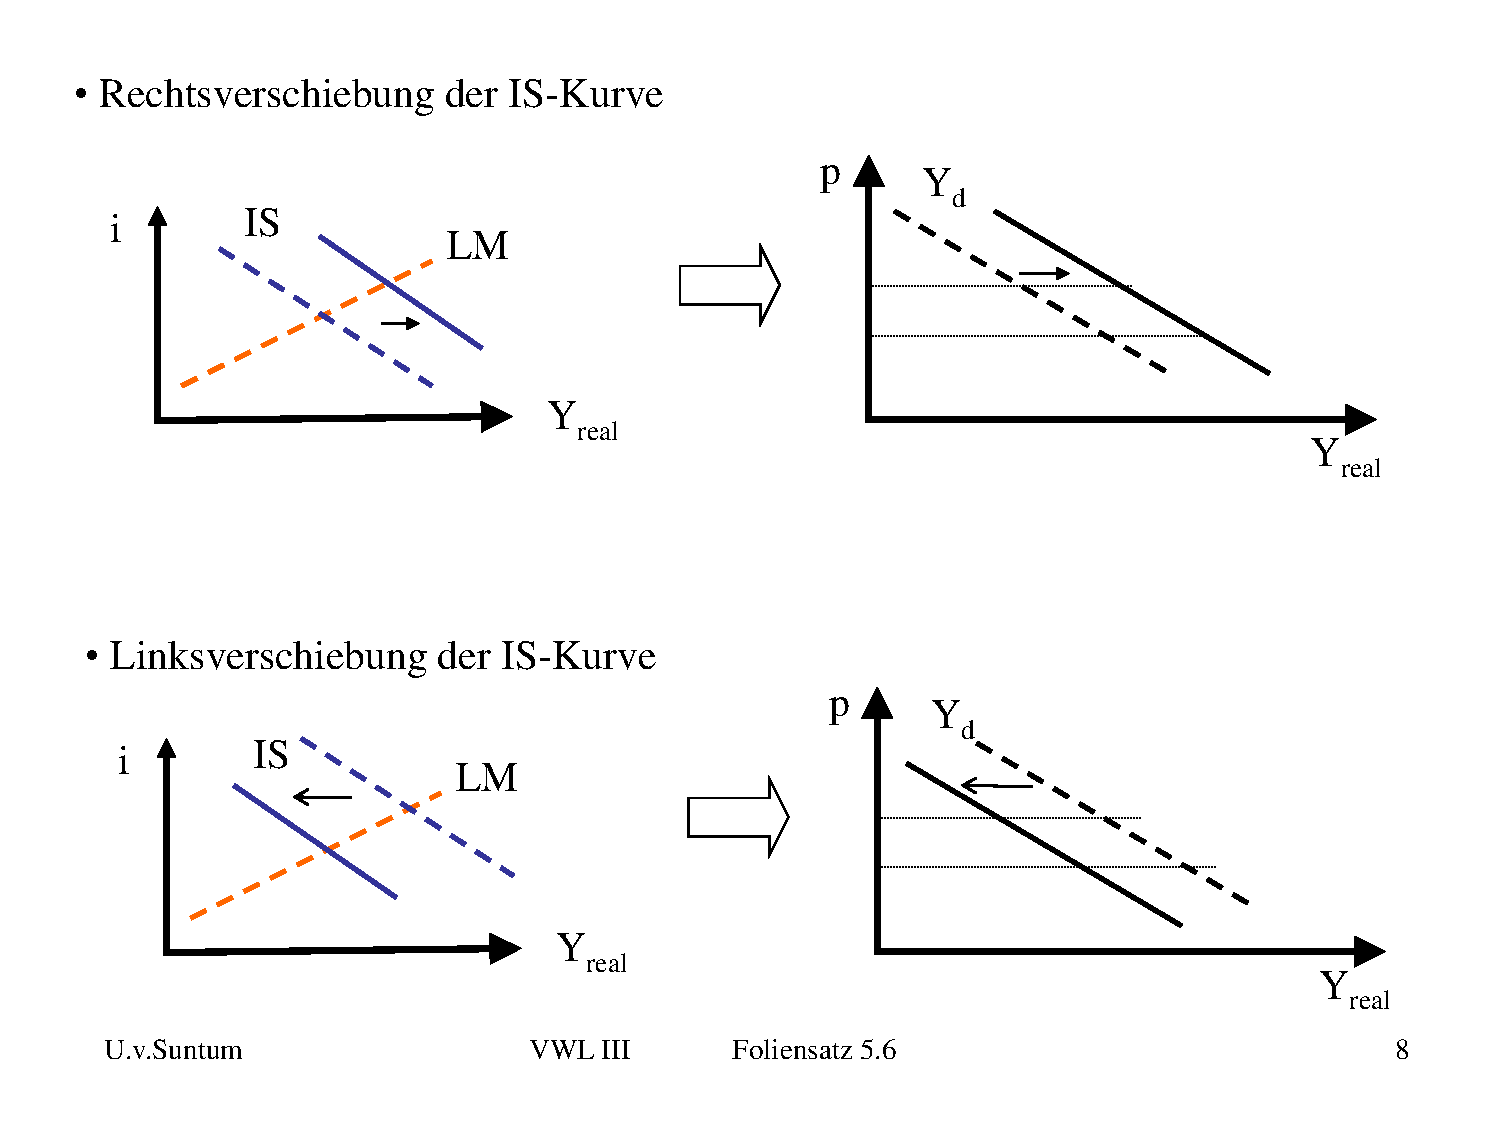
\includegraphics[width=0.8\textwidth]{Bilder/ADLage1.pdf}\\
      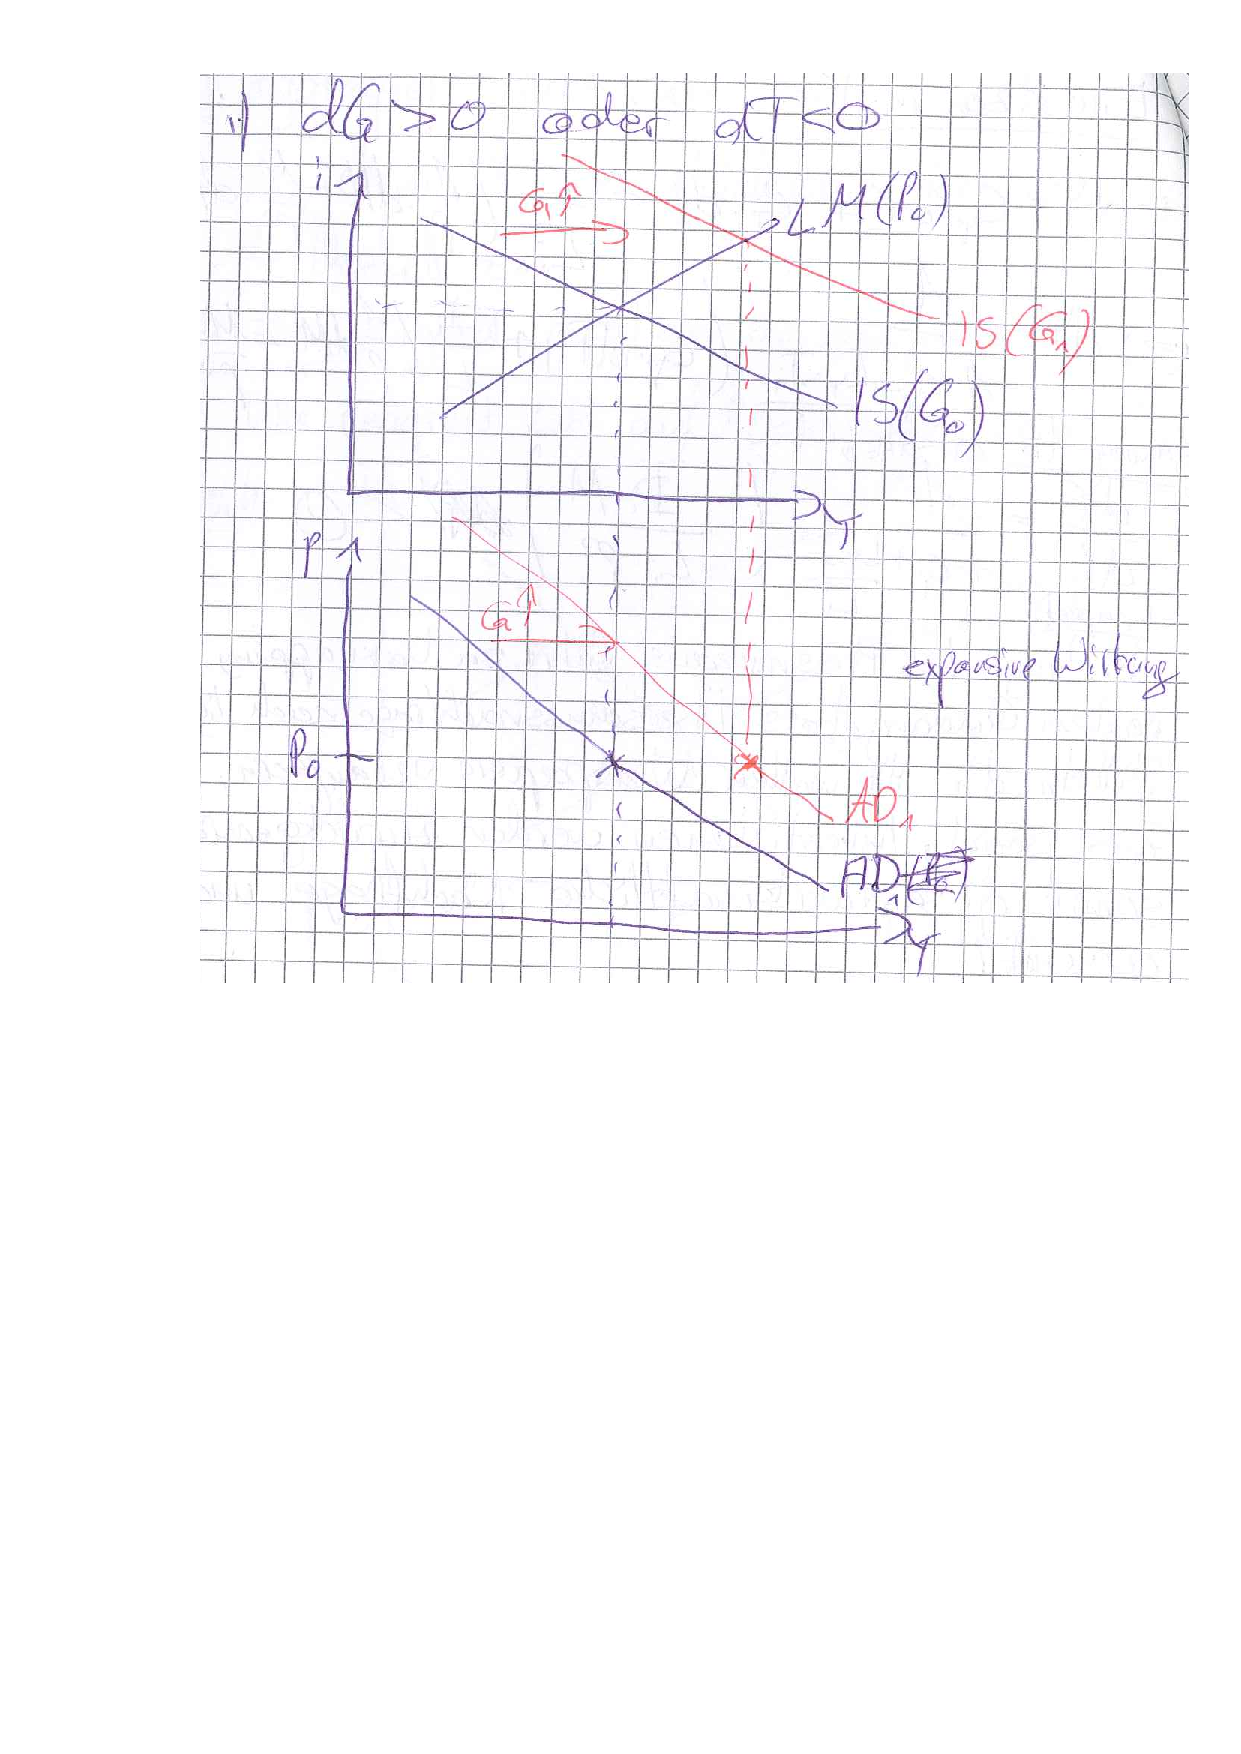
\includegraphics[width=0.8\textwidth]{Bilder/ADLage11.pdf}\\
    \item $dM >0$\\
        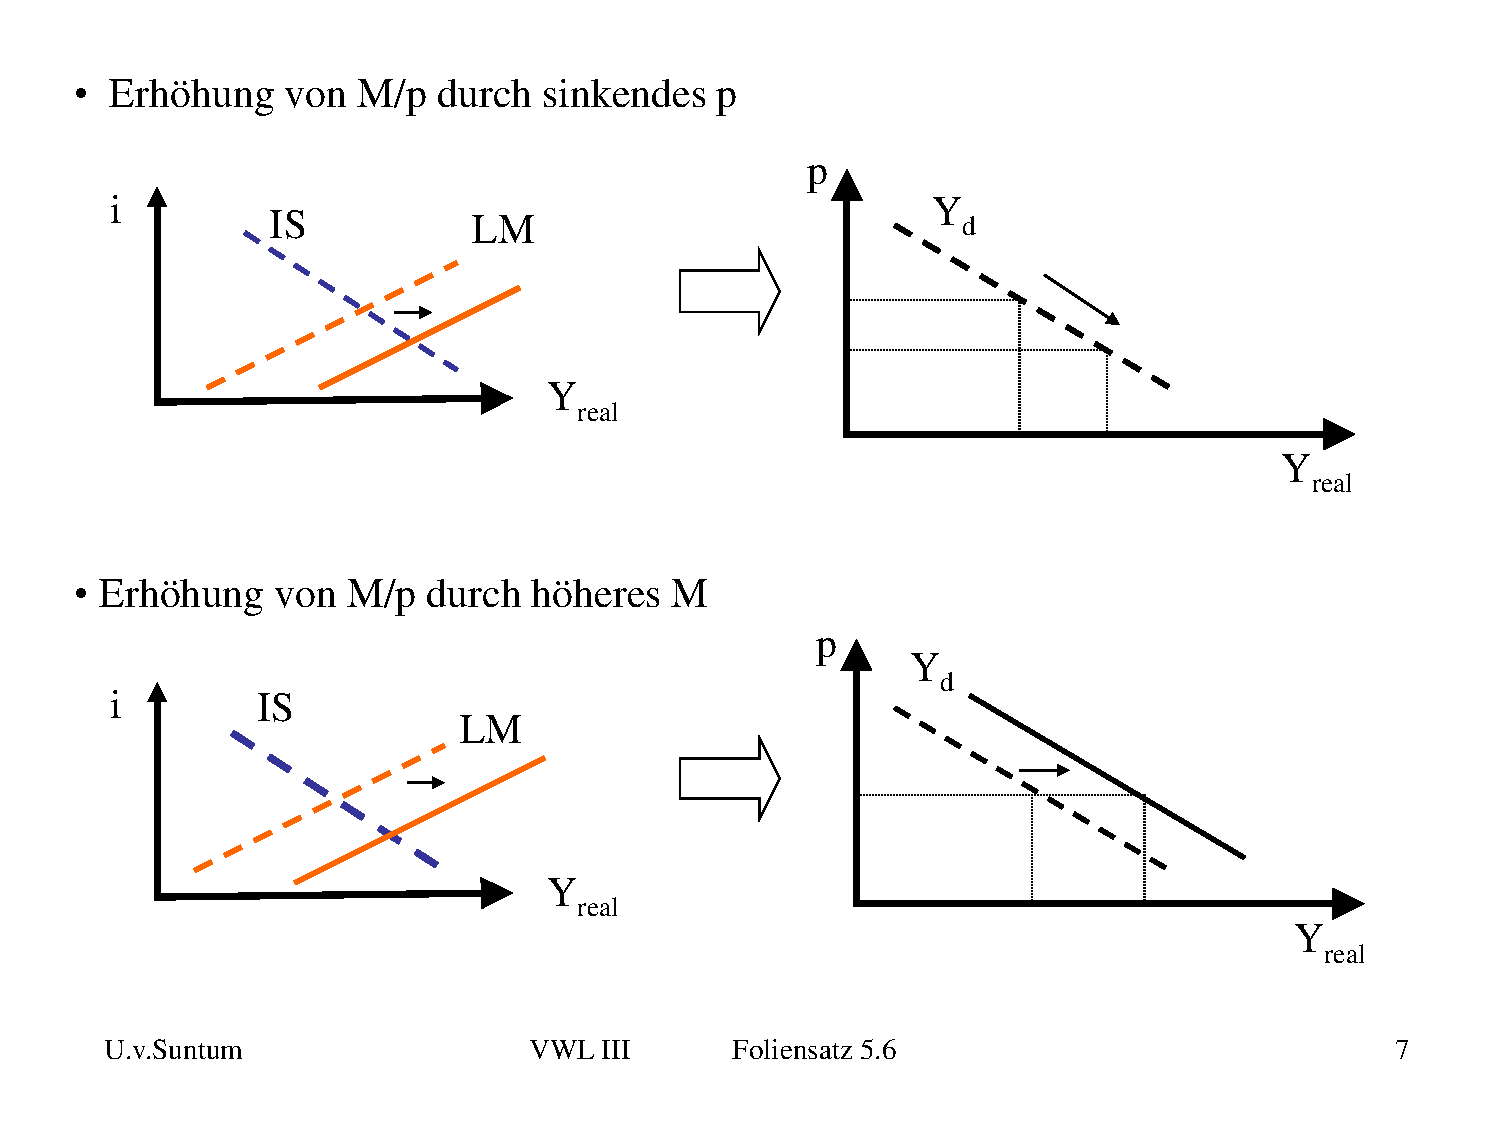
\includegraphics[width=0.8\textwidth]{Bilder/ADLage2.pdf}\\
        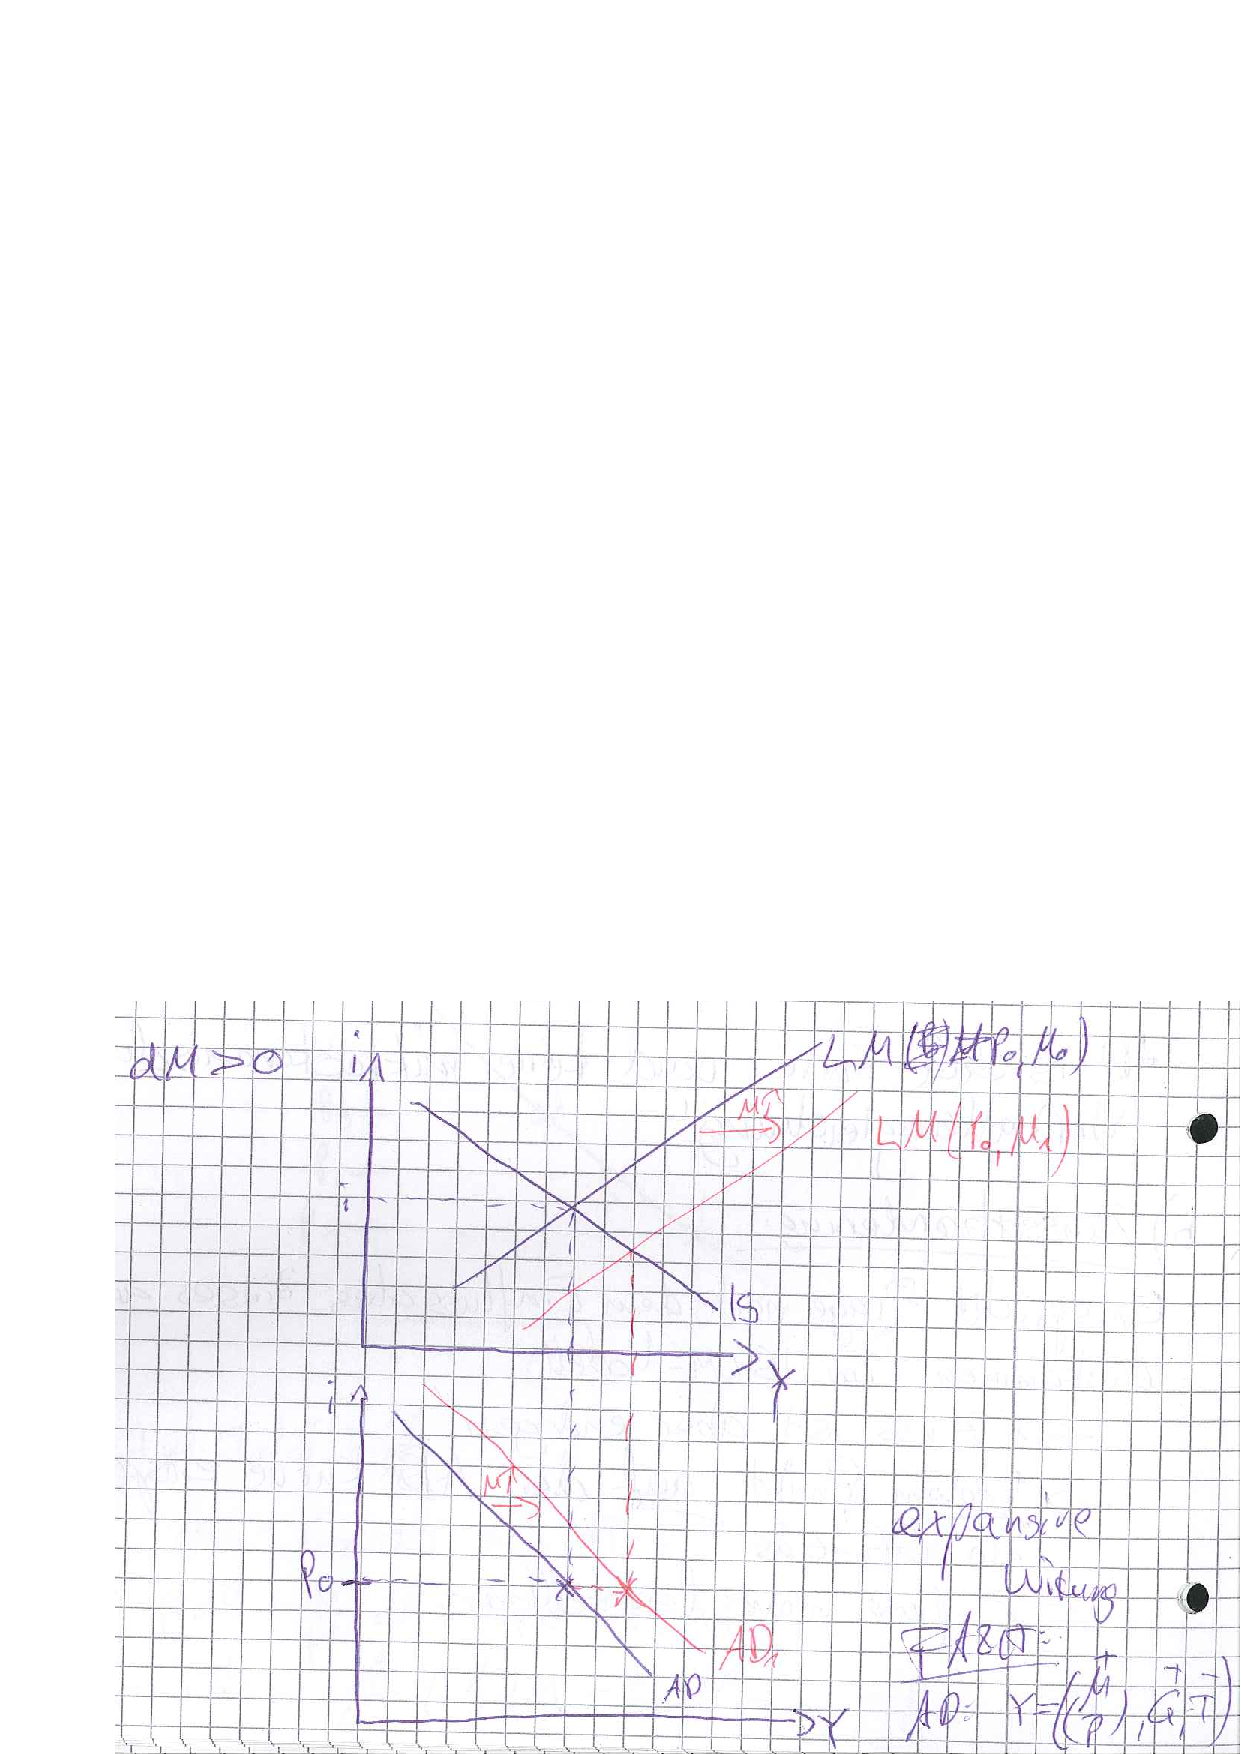
\includegraphics[width=0.8\textwidth]{Bilder/ADLage22.pdf}\\
  \end{enumerate}
  FAZIT: $Y=Y^{AD}(\underbrace{\overset{+}{M},\overset{+}{G},\overset{-}{T}}_\text{Verschiebungen Kurve},\underbrace{\overset{-}{P}}_\text{Auf Kurve})$
\end{enumerate}
\newpage
\subsection{ Wirtschaftspolitische Ma{\ss}nahmen im AS-AD Modell}
\begin{enumerate}[a)]
  \item IS nach i umformen und in LM einsetzen, dann nach P umformen:
  Die AD Kurve fasst den G\"{u}ter- und Geldmarkt zusammen:
  \begin{align*}
    \text{IS}:& Y = C+ I + G\\
    \text{einsetzen}:& Y = 750 + 0.8(Y-750) - 4000 i +750\\
    \text{aufl\"{o}sen}:& 1000 i = 255 - 1/20 Y\\
    \text{in LM}:& M-P = 1/5 Y - 255 + 1/20 Y\\
    \text{AD}:& P = 225 + M - 1/4Y
  \end{align*}
  \item Bei korrekten Erwartungen ist der Arbeitsmarkt im GG, AS-Kurve ist vertikal, d.h. $Y=\bar{Y}$. Preisniveau aus AD-Kurve: $P=250+600-1/4 \cdot 1200 = 550$. Zins aus LM: $1000 i = 255 - 1/20 Y \Leftrightarrow i=0.19$.
  \begin{center}
  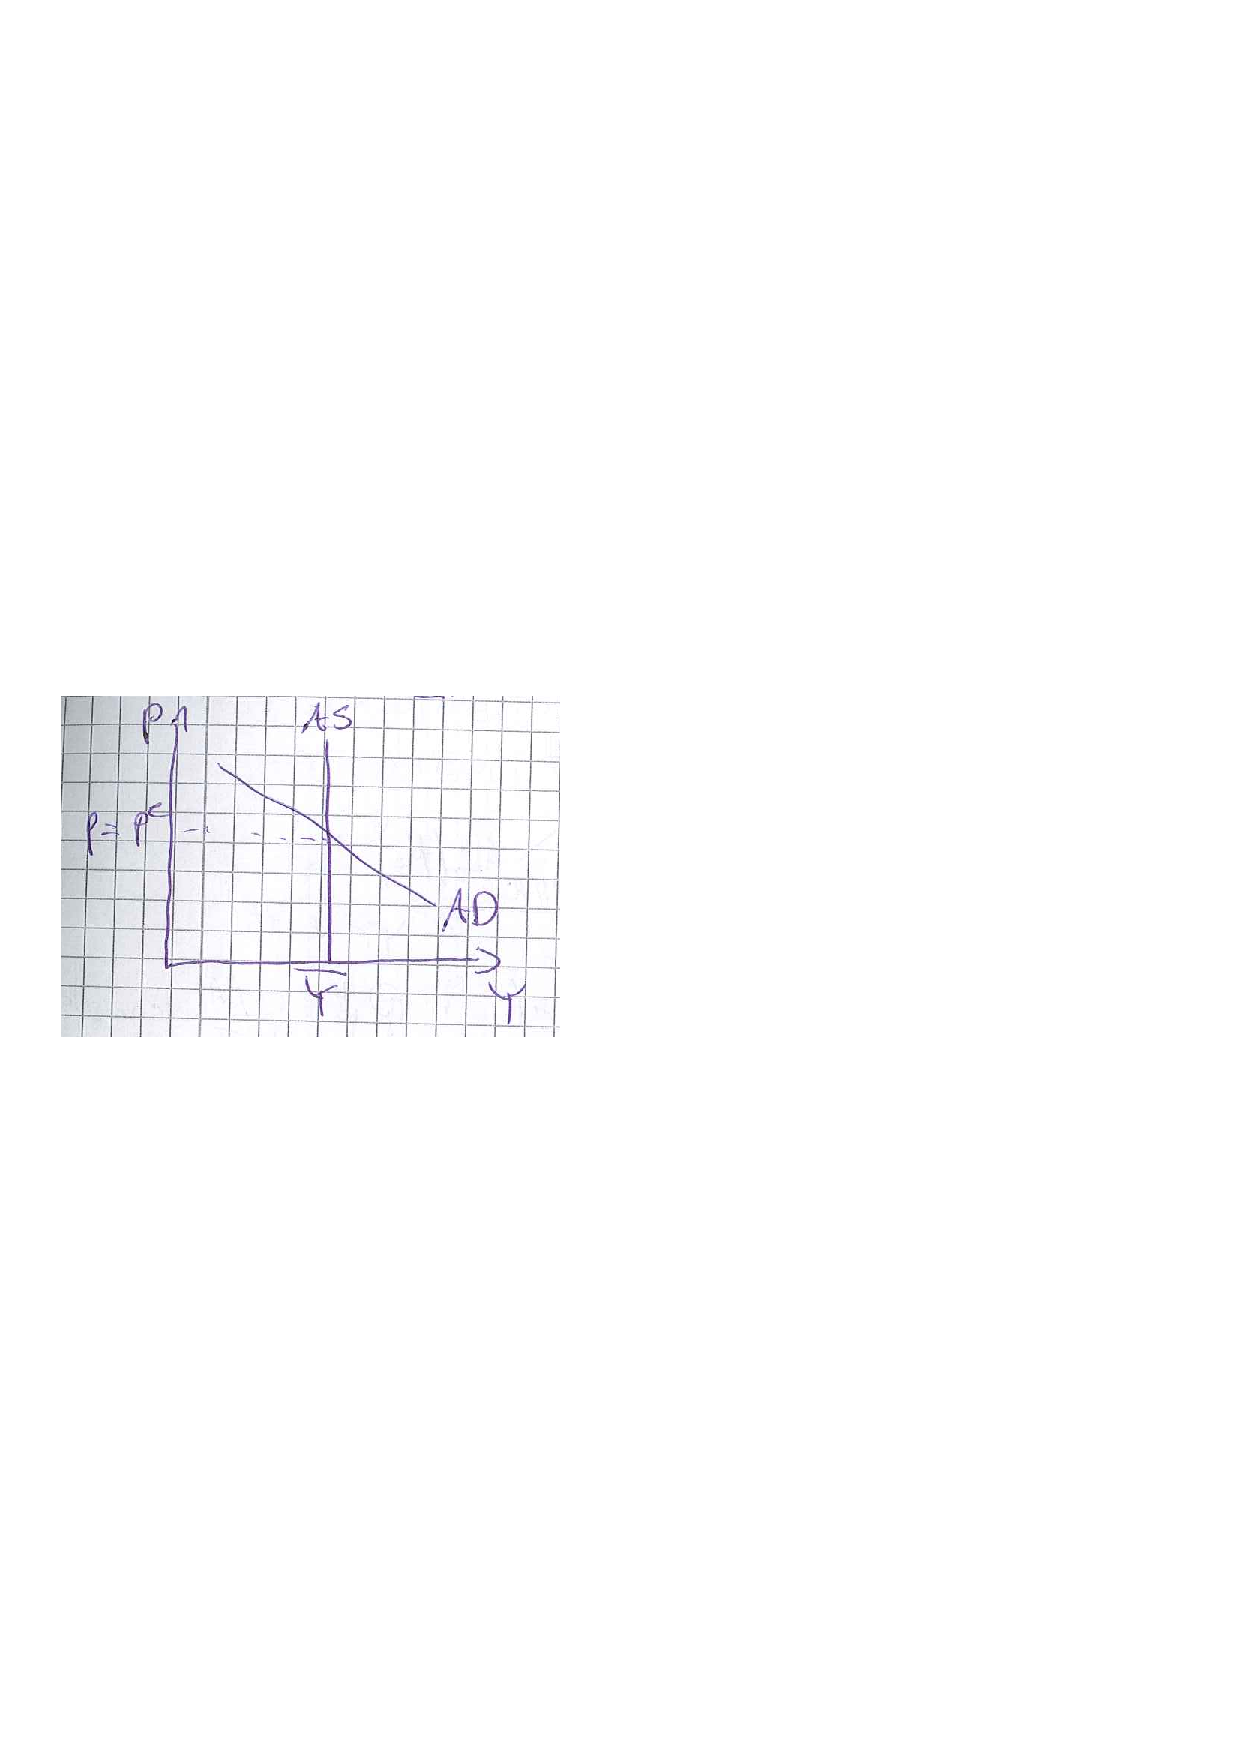
\includegraphics[width=0.5\textwidth]{Bilder/ASAD1.pdf}
  \end{center}
  \item Kontraktive Geldpolitik $M\downarrow$ bei korrekten Preiserwartungen $P=P^e$ (AS senkrecht). Aus AD berechnen wir neues, niedrigeres Preisniveau: $$ P = 250+400-1/4\cdot1200=350$$ Da AS-Kurve unabh\"{a}ngig vom Preisniveau ist, wird der Output am Arbeitsmarkt bestimmt, d.h. Preise fallen. Der Effekt kontraktiver Geldpolitk wird r\"{u}ckg\"{a}ngig gemacht, Zins bleibt konstant.\\
      $M\downarrow \rightarrow i \uparrow \rightarrow I \downarrow \rightarrow Y^d \downarrow \rightarrow Y^d < Y^n$ (AD-Kurve verschiebt sich mit LM). ABER: $N^d \downarrow \rightarrow u \uparrow \rightarrow W \downarrow \rightarrow P \downarrow$ Nominall\"{o}hne und Preise sinken! $P<P^e \Rightarrow P^e \downarrow$! $P\downarrow \rightarrow \frac{M}{P} \uparrow \rightarrow M^s > M^d \rightarrow i \downarrow \rightarrow I \uparrow \rightarrow Y^d \uparrow$
        \begin{center}
  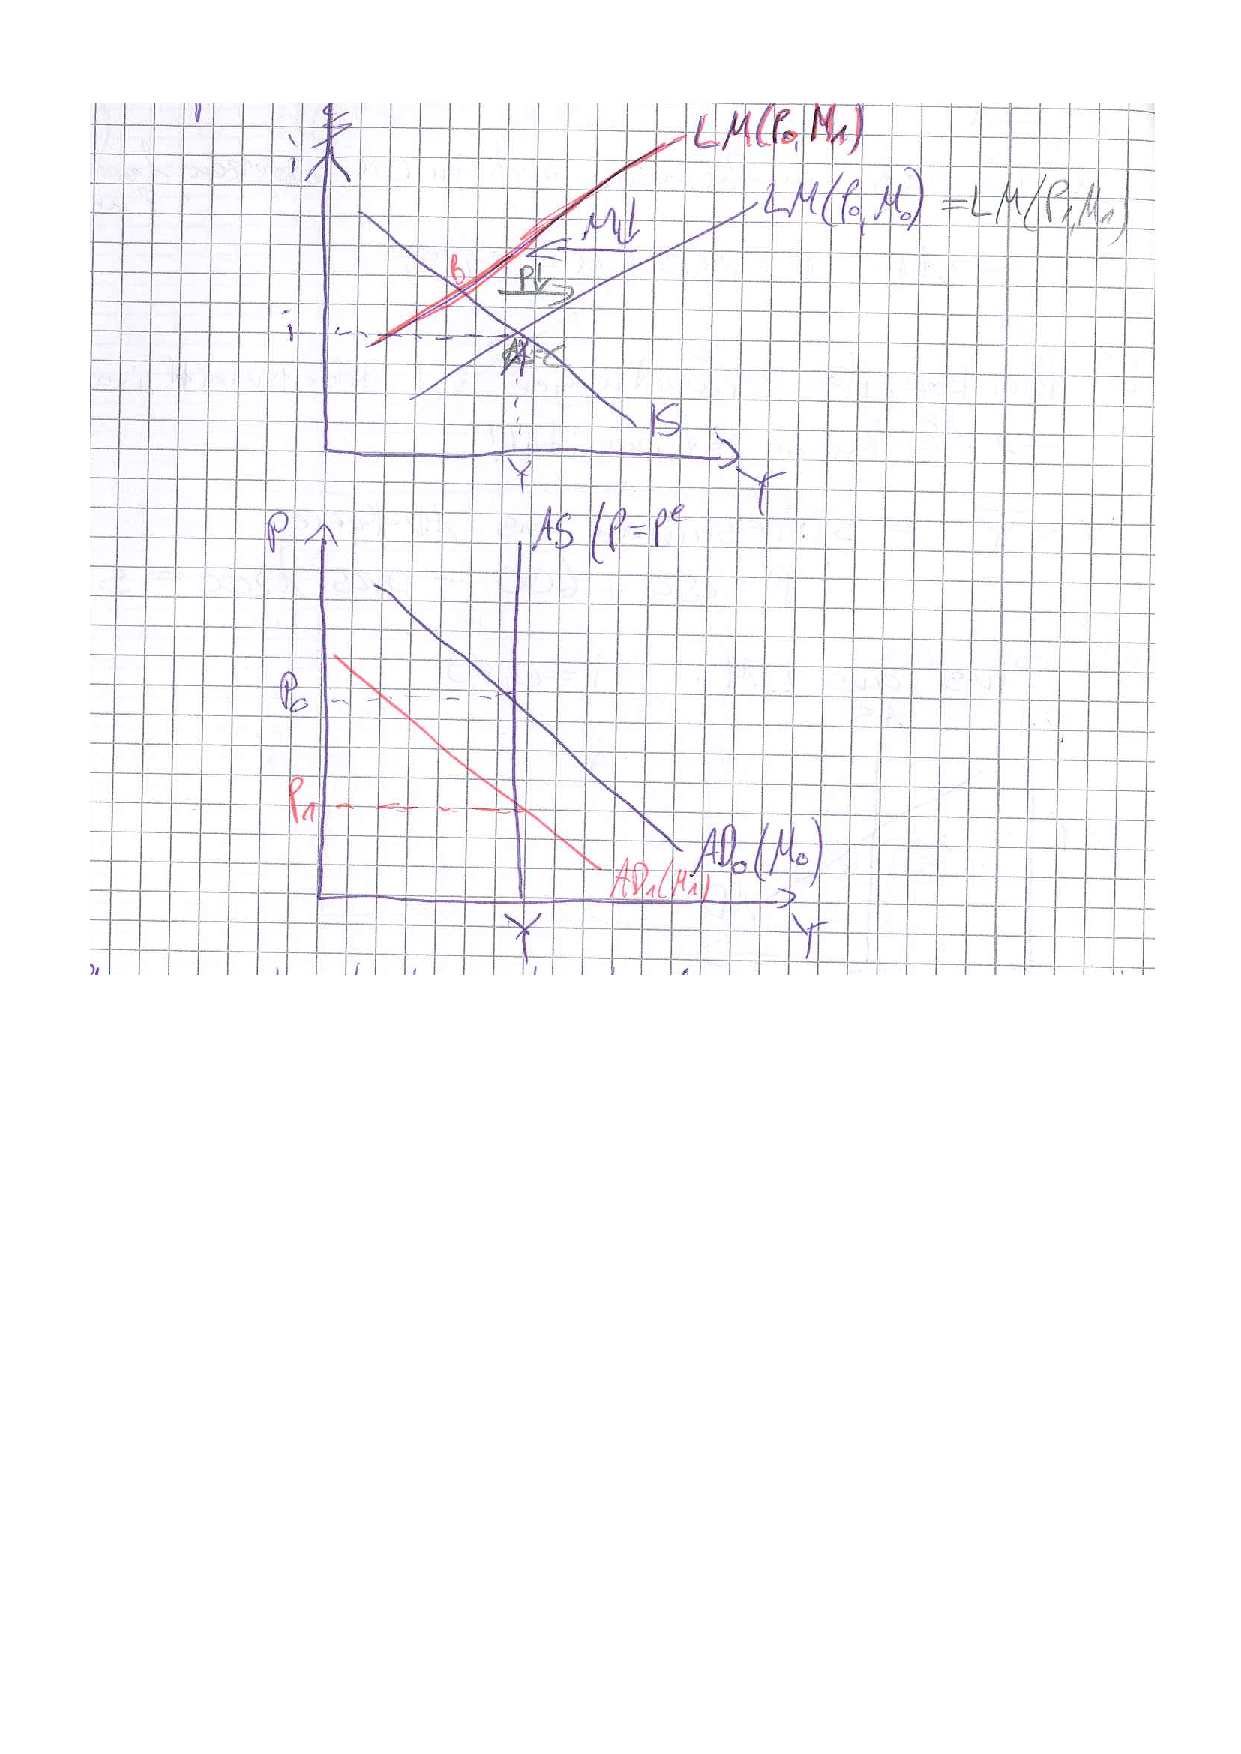
\includegraphics[width=\textwidth]{Bilder/ASAD2.pdf}
  \end{center}
  Fazit: Y konstant, i konstant, Preise sinken, $\frac{M}{P}$ konstant. Dies nennt man Neutralit\"{a}t des Geldes in der mittleren bzw. langen Frist!
  \item Kurze Frist, gegeben konstante Erwartungen!
  $$AD: P = 250+400-1/4Y \Leftrightarrow Y = 2600-4P$$
  Einsetzen in AS (mit $P^e=550$ vor geldpolitischer Ma{\ss}nahme):
  $$ P = 550 + 0.5(2600-4P-1200) \Leftrightarrow P = 416,7, Y = 933,2$$
  Idee: Output wird hier nicht allein am Arbeitsmarkt bestimmt! Kontraktive Geldpolitik f\"{u}hrt zu Senkung des Outputs, damit nimmt Besch\"{a}ftigung und Lohnforderungsmacht ab, dies f\"{u}hrt schie{\ss}lich zu geringeren L\"{o}hnen und Preisen.
          \begin{center}
  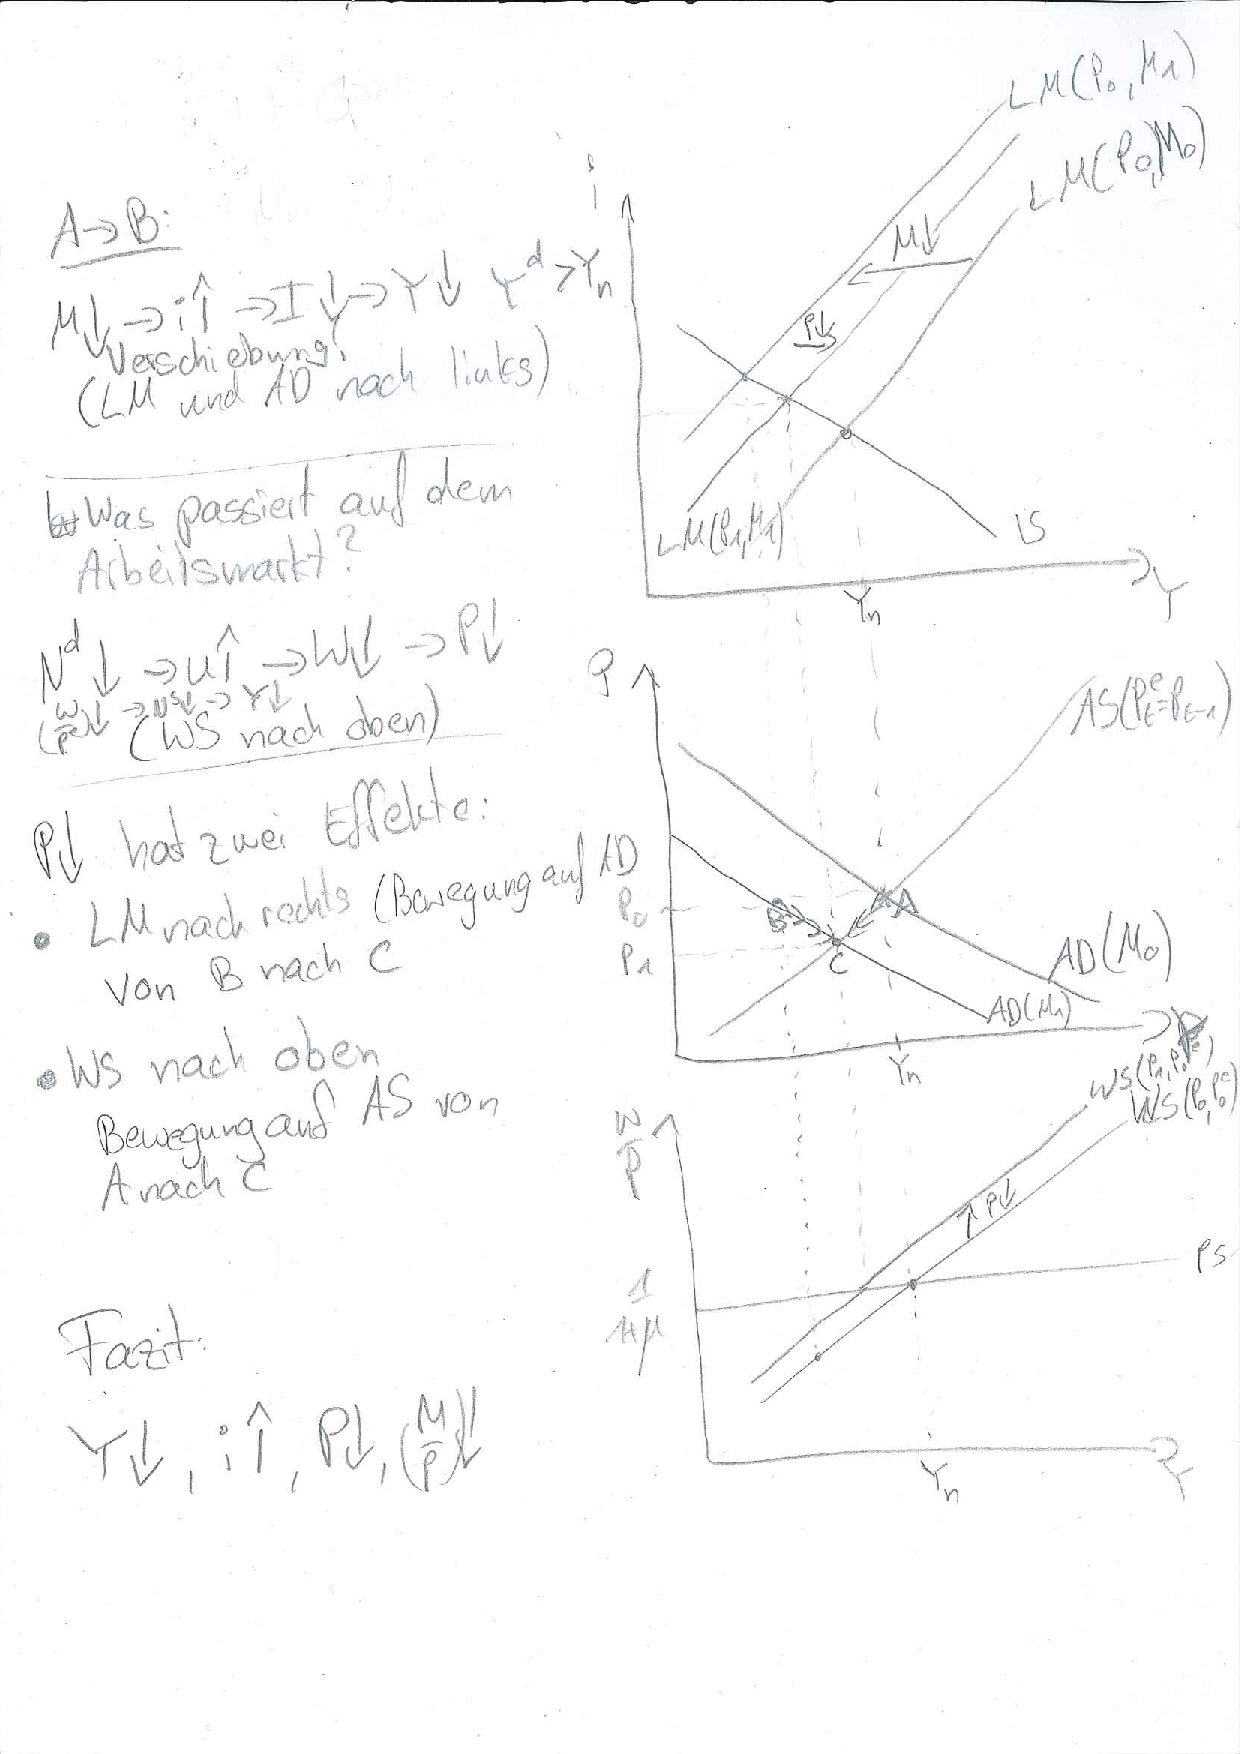
\includegraphics[width=0.9\textwidth]{Bilder/ASAD3.pdf}
  \end{center}
\end{enumerate}

\section{Phillips-Kurve}
Grundidee: Zusammenhang zwischen Inflation und Arbeitslosigkeit, hergeleitet aus der AS-Kurve.
\begin{enumerate}[a)]
  \item Urspr\"{u}nglich negativer Zusammenhang zwischen Nominallohn-Steigerungsrate und der Arbeitslosenquote. $$ \hat{W_t} =  \frac{dW_t}{W_{t-1}} =  \frac{W_t-W_{t-1}}{W_{t-1}} = \alpha (u_{n}-u_t), \alpha >0$$
  \"{O}konomischer Mechanismus: Sinkende Arbeitslosigkeit sorgt f\"{u}r eine Erh\"{o}hung der L\"{o}hne. Die Kosten der Unternehmen steigen somit, Preise werden erh\"{o}ht, in anderen Worten, es gibt Inflation!\\
  Sp\"{a}ter: Ersetzung der Nominallohn-Steigerungsrate durch Inflation und Erwartungsbildung.\\
  Lohn-Preis-Spirale: Arbeitslosigkeit f\"{a}llt, Nominall\"{o}hne steigen, Kosten der Unternehmen steigen, Preise werden erh\"{o}ht. Aufgrund steigender Preise werden Arbeiter sp\"{a}ter noch h\"{o}here Nominall\"{o}hne verlangen, was wiederum zu h\"{o}heren Preisen f\"{u}hrt....
  \item AS: $P_t = P_t^e(1+\mu)F(u_t,z)$ durch $P_{t-1}$ teilen:
  \begin{align*}
    \frac{P_t}{P_{t-1}} = \frac{P_t^e}{P_{t-1}} (1+\mu) = F(u_t,z)\\
    \Leftrightarrow 1+\pi_t = (1+\pi_t^e) (1+\mu) F(u_t,z) \\
    \Leftrightarrow \frac{1+\pi_t}{(1+\pi_t^e) (1+\mu)} = F(u_t,z)\\
  \end{align*}
  Nun gelten folgende Approximationen f\"{u}r kleine Werte, d.h. f\"{u}r Werte zwischen 0 und 10\%: $x,y \in [0;0.1]:$
  \begin{align*}
    1.& (1+x)(1+y) = 1+x+y +xy \approx 1+x+y, \text{ da } xy \in[0;0.01]\\
    2.& \frac{1+x}{1+y} \approx 1+x -y, \text{ da }\\ &(1+x-y)(1+y)=1+x-y+y+xy +y^2, \text{ mit } xy \in[0;0.01], y^2 \in[0;0.01]
  \end{align*}
  Somit
  \begin{align*}
    1 + \pi_t - \pi_t^e - \mu = F(u_t,z) = 1-\alpha u_t + z\\
    \Leftrightarrow \pi_t = \pi_t^e + \underbrace{(\mu+z)}_{\alpha u_n} - \alpha u_t
  \end{align*}
  Die nat\"{u}rliche Arbeitslosenquote wird nur durch $\mu$ und $z$ bestimmt!
  \item Kurzfristige PC: Tradeoff zwischen Inflation und Arbeitslosigkeit\\
  Langfristige bzw. mittelfristige PC: In der langen bzw. mittleren Frist gilt immer strukturelle nat\"{u}rliche Arbeitslosigkeit bei beliebiger Inflation!
    \begin{center}
  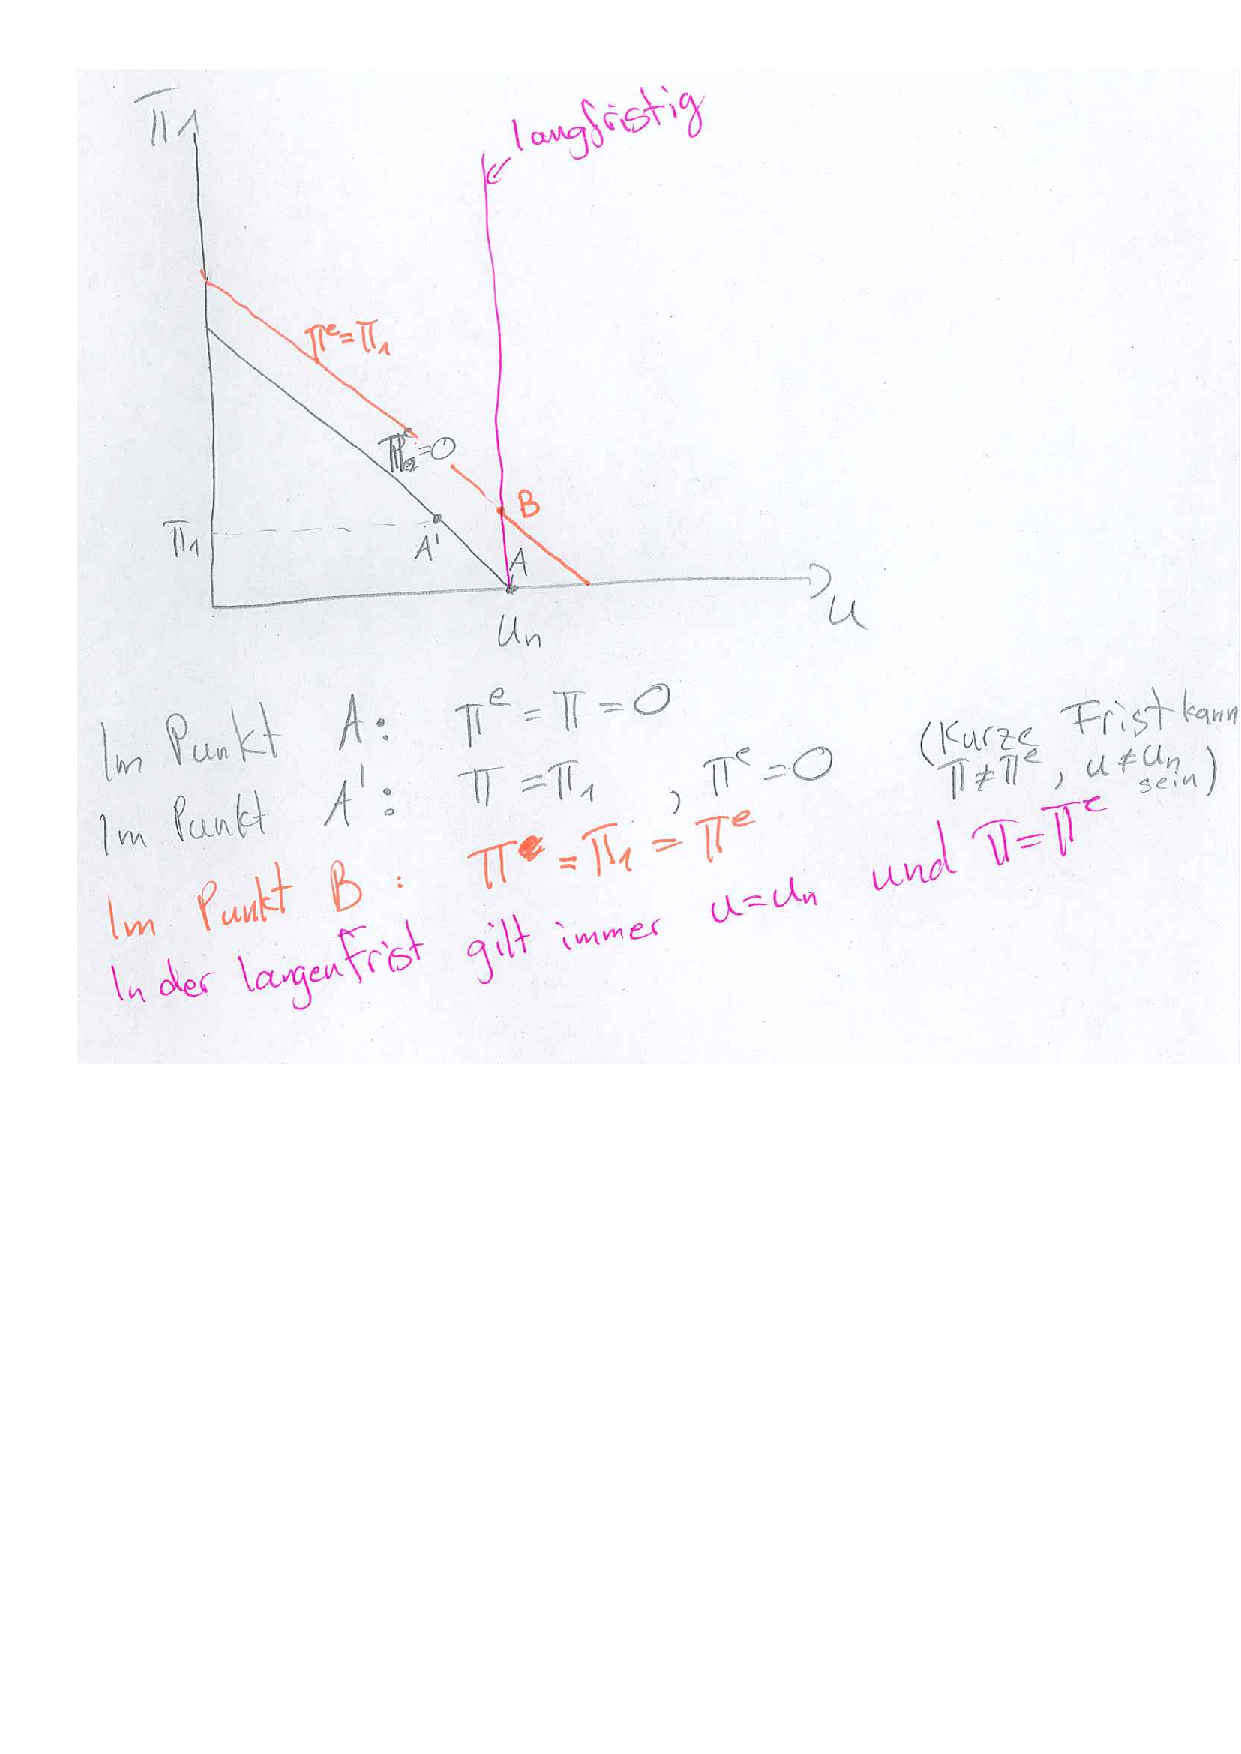
\includegraphics[width=\textwidth]{Bilder/PhillipsKurve.pdf}
  \end{center}

  \item
  \begin{enumerate}[(i)]
    \item Dies ist die um Erwartungen erweiterte Phillipskurve. Wenn die aktuelle Arbeitslosenquote gleich ihrem nat\"{u}rlichen Niveau, sind aktuelle Inflation gleich den Inflationserwartungen. Inflation wird sich in diesem Fall nicht \"{a}ndern. Falls die aktuelle Arbeitslosenquote unterhalb der nat\"{u}rlichen liegt, wird die Inflation positiv sein, d.h. Preise steigen. Die nat\"{u}rliche Arbeitslosenquote wird deshalb auch als NAIRU (non-accelerating-inflation-rate-of-unemployment) bezeichnet.
    \item \begin{itemize}
      \item Statische Erwartungen: $\pi_t^e = 0$: Urspr\"{u}ngliche Phillipskurve, negativer Zusammenhang zwischen Arbeitslosenquote und Inflation
      \item Adaptive Erwartungen: $\pi_t^e = \theta \pi_{t-1} \Rightarrow \pi_t - \theta \pi_{t-1} = \alpha(u_n-u)$ Arbeitslosenquote beeinflusst die Ver\"{a}nderungsrate der Inflation, nicht das Niveau. Inflationserwartungen werden hier immer nur im Nachhinein (ex post) auf der Basis der Inflation der Vorperiode angepasst. Geldpolitik kann in einem solchen Umfeld, die Reall\"{o}hne durch steigende Inflation wiederholt senken, und den Arbeitsmarkt dadurch dauerhaft beleben.
      \item Rationale Erwartungen: $\pi_t^e = \pi_t + \varepsilon_t$ mit $E_{t-1}(\varepsilon_t)=0$. Alle zur Verf\"{u}gung stehenden Informationen (ex ante) werden genutzt!
      Idee: Unsinn, dass Akteure dauerhaft systematische Erwartungsfehler machen und nicht daraus lernen. Phillips-kurve wird dann
      $$ u_t = u_n - \frac{1}{\alpha} \varepsilon_t$$
      Zusammenhang zur Inflation nicht mehr vorhanden! Selbst kurzfristig ist Phillipskurve vertikal! (Glaubw\"{u}rdige) Geldpolitische Politikma{\ss}nahmen sind dann nicht nur mittelfristig,
      sondern sogar kurzfristig neutral.
      \item Kritik an Rationalen Erwartungen: Begrenzte Rationalit\"{a}t und Nominale Rigidit\"{a}ten, d.h. z.B
      $$ \pi_t^e = \lambda \pi_t + (1-\lambda) \pi_{t-1}, \lambda \in [0;1]$$
      $\lambda$ ist Anteil derjenigen, die rationale Erwartungen haben bzw. ihre Preise/L\"{o}hne neu verhandeln k\"{o}nnen. Somit folgt f\"{u}r die PC:
      $$ \pi_t - \pi_{t-1} = \frac{\alpha}{1-\lambda}(u_n-u_t)$$
      $\lambda$ ist Ma{\ss} f\"{u}r Rationalit\"{a}t und im Zeitverlauf ver\"{a}nderbar (Lucas Kritik). Je h\"{o}her $\lambda$ desto steiler ist die PC und Geldpolitik hat kurzfristig auch eher keinen Einfluss
    \end{itemize}
  \end{enumerate}
\end{enumerate}

\newpage
\section{Solow-Modell}
\subsection*{Verst\"{a}ndnis}
Neoklassisches Wachstumsmodell: Identifiziert Kapitalakkumulation und technischen Fortschritt als Determinanten des Wachstums, und liefert eine Erkl\"{a}rung
f\"{u}r die Konvergenzhypothese, d.h. den Aufholprozess (hohe vor\"{u}bergehende Wachstumsraten, die mit der Zeit sinken und auf ein konstantes Niveau einpendeln)\\
Wichtige Erkenntnisse:
\begin{itemize}
  \item Erh\"{o}hung gesamtwirtschaftlicher Ersparnis und Investition f\"{u}hrt zu einer vor\"{u}bergehenden, nicht aber zu einer dauerhaften Beschleunigung des pro-Kopf Wirtschaftswachstums.
  \item Dauerhaftes pro-Kopf Wachstum nicht ohne technischen Fortschritt denkbar ist.
\end{itemize}
Wir unterscheiden 2 Modellvarianten: Einfaches Solow Modelle (ohne Bev\"{o}lkerungswachstum, ohne Wachstum technischen Fortschritts) und Solow-Modell mit Labor-Augmenting technischen Fortschritts mit Bev\"{o}lkerungswachstum und Effizienz der Arbeit f\"{o}rdernden technischen Fortschritt.
Wichtige Gleichungen:
\begin{enumerate}
\item Einfaches Solow Modell
\begin{itemize}
  \item Produktionsfunktion vom Typ Cobb-Douglas: $Y_t = A K_t^\alpha N^{1-\alpha}$.
  \item Kapitalakkumulationsgleichung: $$K_{t+1}=(1-\delta)K_t + s Y_t$$
  Neue Kapitalstock $K_{t+1}$ ist gleich dem alten Kapitalstock $K_t$ abz\"{u}glich dem abgeschriebenen $\delta K_t$ und zus\"{a}tzlich der Ersparnis (= Investition) $sY_t$
  \item Betrachte Gleichungen in pro-Kopf-Notation: $y_t = \frac{Y_t}{N}$ und $k_t = \frac{K_t}{N}$, also:
      \begin{align*}
        y_t &= \frac{Y_t}{N} = A \frac{K_t^\alpha N^{1-\alpha}}{N^\alpha N^{1-\alpha}} = A \left(\frac{K_t}{N}\right)^\alpha = A k_t^\alpha\\
        k_{t+1} &= \frac{K_{t+1}}{N} = (1-\delta)\frac{K_t}{N} + s \frac{Y_t}{N} = (1-\delta)k_t + s y_t = (1-\delta)k_t + s A k_t^\alpha
      \end{align*}
  \item Steady-State: Gleichgewicht, in dem sich die Kapitalintensit\"{a}t $k_t$ und pro-Kopf Output $y_t$ nicht mehr ver\"{a}ndern, also konstant sind! Setze also $k_t=k_{t+1}=k$ und $y_t=y$. Also erst steady-state Kapitalintensit\"{a}t:
      \begin{align*}
      k &= (1-\delta)k + sAk^\alpha\\
      \Leftrightarrow k & = \left(\frac{sA}{\delta}\right)^{\frac{1}{1-\alpha}}
      \end{align*}
      Einsetzen in $y = A k^\alpha$ gibt steady-state pro-Kopf Output:
      \begin{align*}
        y = A \left(\frac{sA}{\delta}\right)^{\frac{\alpha}{1-\alpha}}
      \end{align*}
      $k$ und $y$ sind IM NIVEAU h\"{o}her, wenn (i) A steigt, (ii) s steigt und (iii) $\delta$ sinkt. Wichtig: Im steady-state gibt es kein Wachstum der Pro-Kopf Gr\"{o}{\ss}en, auch Niveaugr\"{o}{\ss}en ($Y_t$ und $K_t$ wachsen ohne Bev\"{o}lkerungswachstum nicht). Beim Anpassungsprozess zu einem h\"{o}heren Steady-State gibt es Wachstum aller Gr\"{o}{\ss}en!\\
      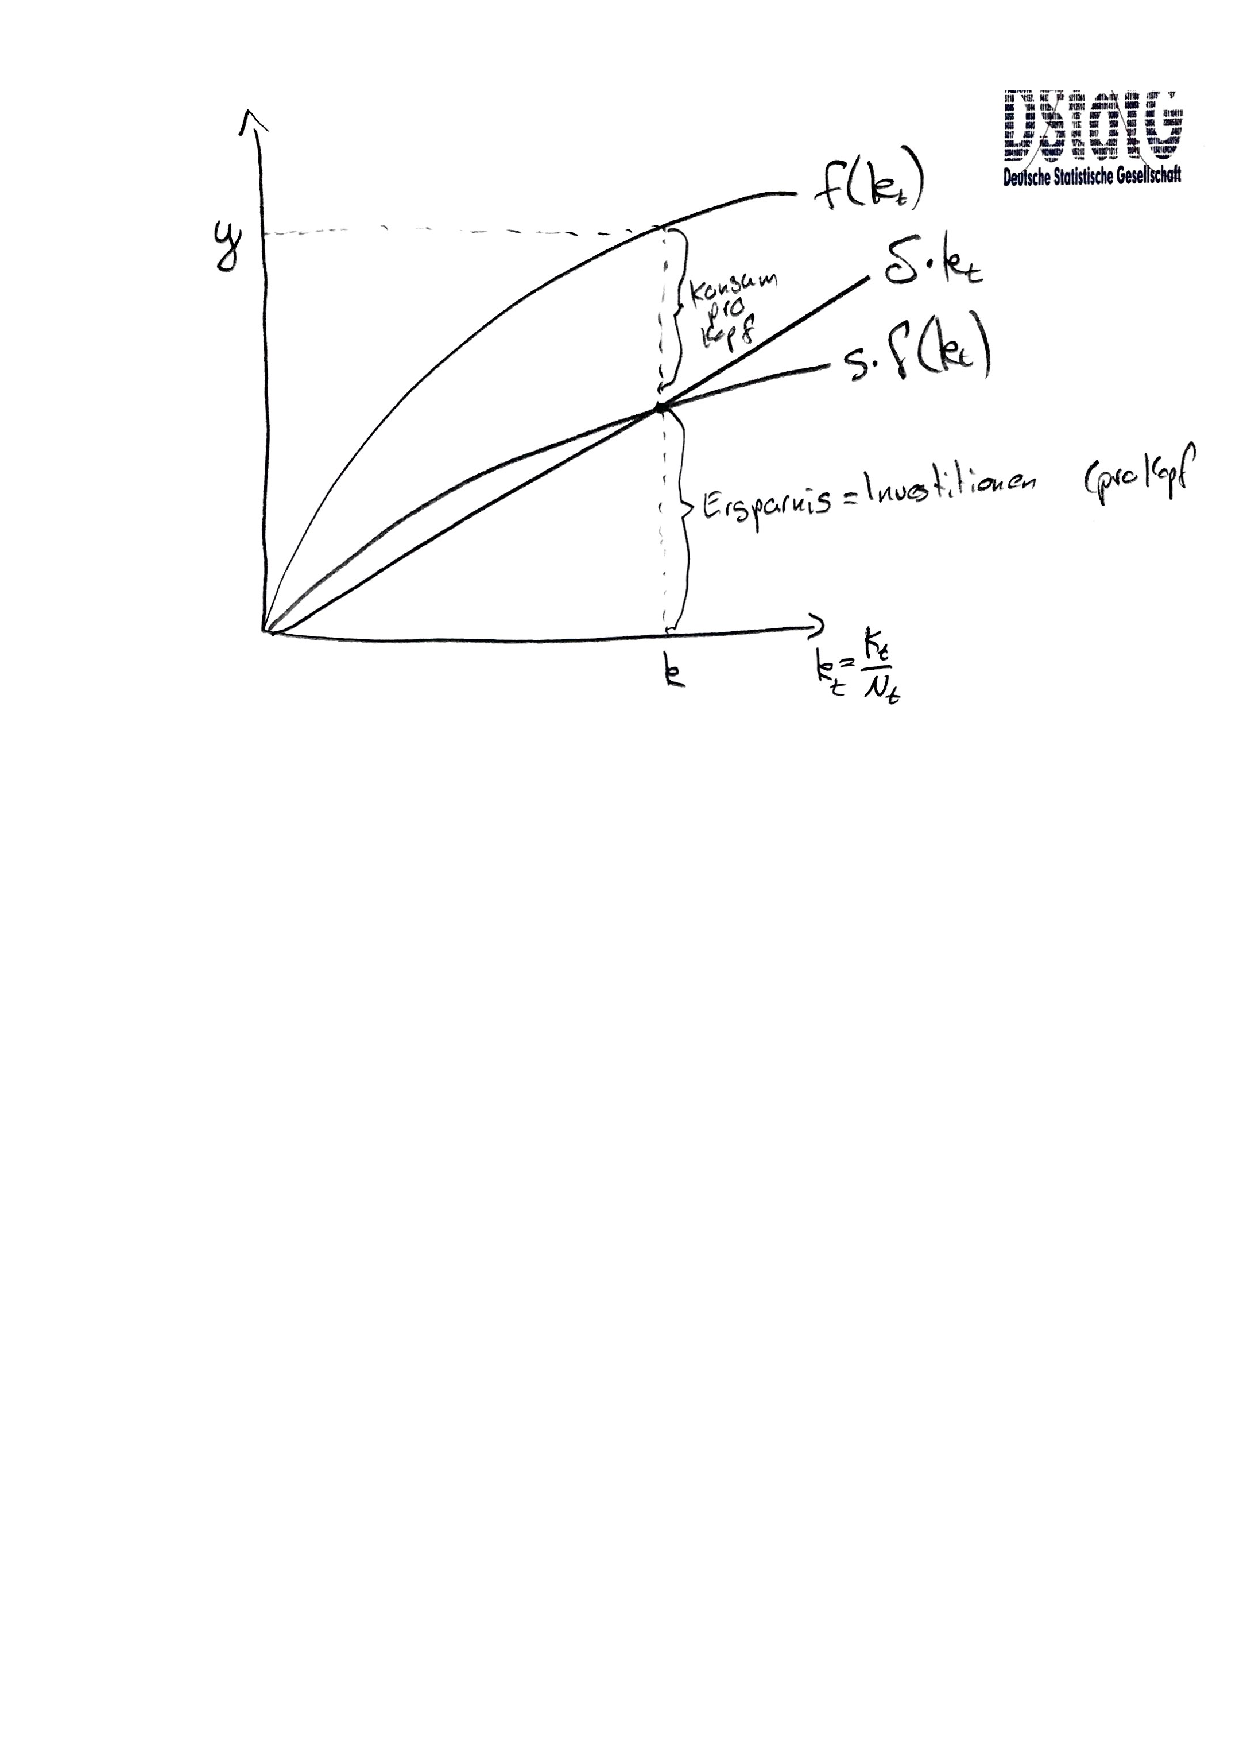
\includegraphics[width=\textwidth,keepaspectratio]{Bilder/Solow1.pdf}
  \item Wann verschiebe ich welche Kurve:
  \begin{itemize}
  \item Technischer Fortschritt steigt: Verschiebung der Kurve $f(k_t)$ nach oben
  \item Sparquote steigt: Pro-Kopf Investition $sf(k_t)$ verschiebt sich nach oben
  \item Abschreibungsrate steigt: Pro-Kopf Abschreibungen $\delta k_t$ dreht sich nach oben
  \end{itemize}
\end{itemize}

\item Solow Modell mit Bev\"{o}lkerungswachstum und labor-augmenting technischen Fortschritts, d.h. $\frac{N_{t+1}}{N_t} = 1+g_N$ und $\frac{A_{t+1}}{A_t} = 1+g_A$
\begin{itemize}
  \item Produktionsfunktion vom Typ Cobb-Douglas: $Y_t = K_t^\alpha \left(A_tN_t\right)^{1-\alpha}$.
  \item Kapitalakkumulationsgleichung: $$K_{t+1}=(1-\delta)K_t + s Y_t$$
  \item Betrachte Gleichungen in Effizienzeinheiten-Notation: $\tilde{y}_t = \frac{Y_t}{A_tN_t}$ und $\tilde{k}_t = \frac{K_t}{A_tN_t}$, also:
      \begin{align*}
        \tilde{y}_t &= \frac{Y_t}{A_tN_t} = \frac{K_t^\alpha (A_tN_t)^{1-\alpha}}{(A_tN_t)^\alpha (A_tN_t)^{1-\alpha}} = \left(\frac{K_t}{A_tN_t}\right)^\alpha = \tilde{k}_t^\alpha\\
        \frac{K_{t+1}}{A_{t}N_{t}} \frac{A_{t+1}N_{t+1}}{A_{t+1}N_{t+1}} &= \tilde{k}_{t+1}(1+g_A)(1+h_N)\\ &= (1-\delta)\frac{K_t}{A_{t}N_{t}} + s \frac{Y_t}{A_{t}N_{t}} = (1-\delta)\tilde{k}_t + s \tilde{y}_t = (1-\delta)\tilde{k}_t + s \tilde{k}_t^\alpha
      \end{align*}
  \item Steady-State: Gleichgewicht, in dem sich der Kapitalstock in Effizienzeinheiten $\tilde{k}_t$ und Output in Effizienzeinheiten $\tilde{y}_t$ nicht mehr ver\"{a}ndern, also konstant sind! Setze also $\tilde{k}_t=\tilde{k}_{t+1}=\tilde{k}$ und $\tilde{y}_t=y$. Also erst steady-state Kapital in Effizienzeinheiten. Beachte hier, dass $(1+g_A)(1+g_N) \approx 1+g_A+g_N$, also:
      \begin{align*}
      \tilde{k}(1+g_A+g_N) &= (1-\delta)\tilde{k} + s\tilde{k}^\alpha\\
      \Leftrightarrow \tilde{k} & = \left(\frac{s}{\delta+g_A+g_N}\right)^{\frac{1}{1-\alpha}}
      \end{align*}
      Einsetzen in $\tilde{y} = \tilde{k}^\alpha$ gibt steady-state Output pro Effizienzeinheit:
      \begin{align*}
        \tilde{y} = \left(\frac{s}{\delta+g_A+g_N}\right)^{\frac{\alpha}{1-\alpha}}
      \end{align*}
      $\tilde{k}$ und $\tilde{y}$ sind IM NIVEAU h\"{o}her, wenn (i) das Wachstum der Technologie oder Bev\"{o}lkerungswachstum sinkt, (ii) s steigt und (iii) $\delta$ sinkt. Wichtig: Im steady-state gibt es kein Wachstum der Effizienzeinheiten Gr\"{o}{\ss}en, ABER: pro-Kopf Gr\"{o}{\ss}en wachsen nun mit der Rate des technischen Fortschritts und die Niveaugr\"{o}{\ss}en mit $g_A+g_N$\\
      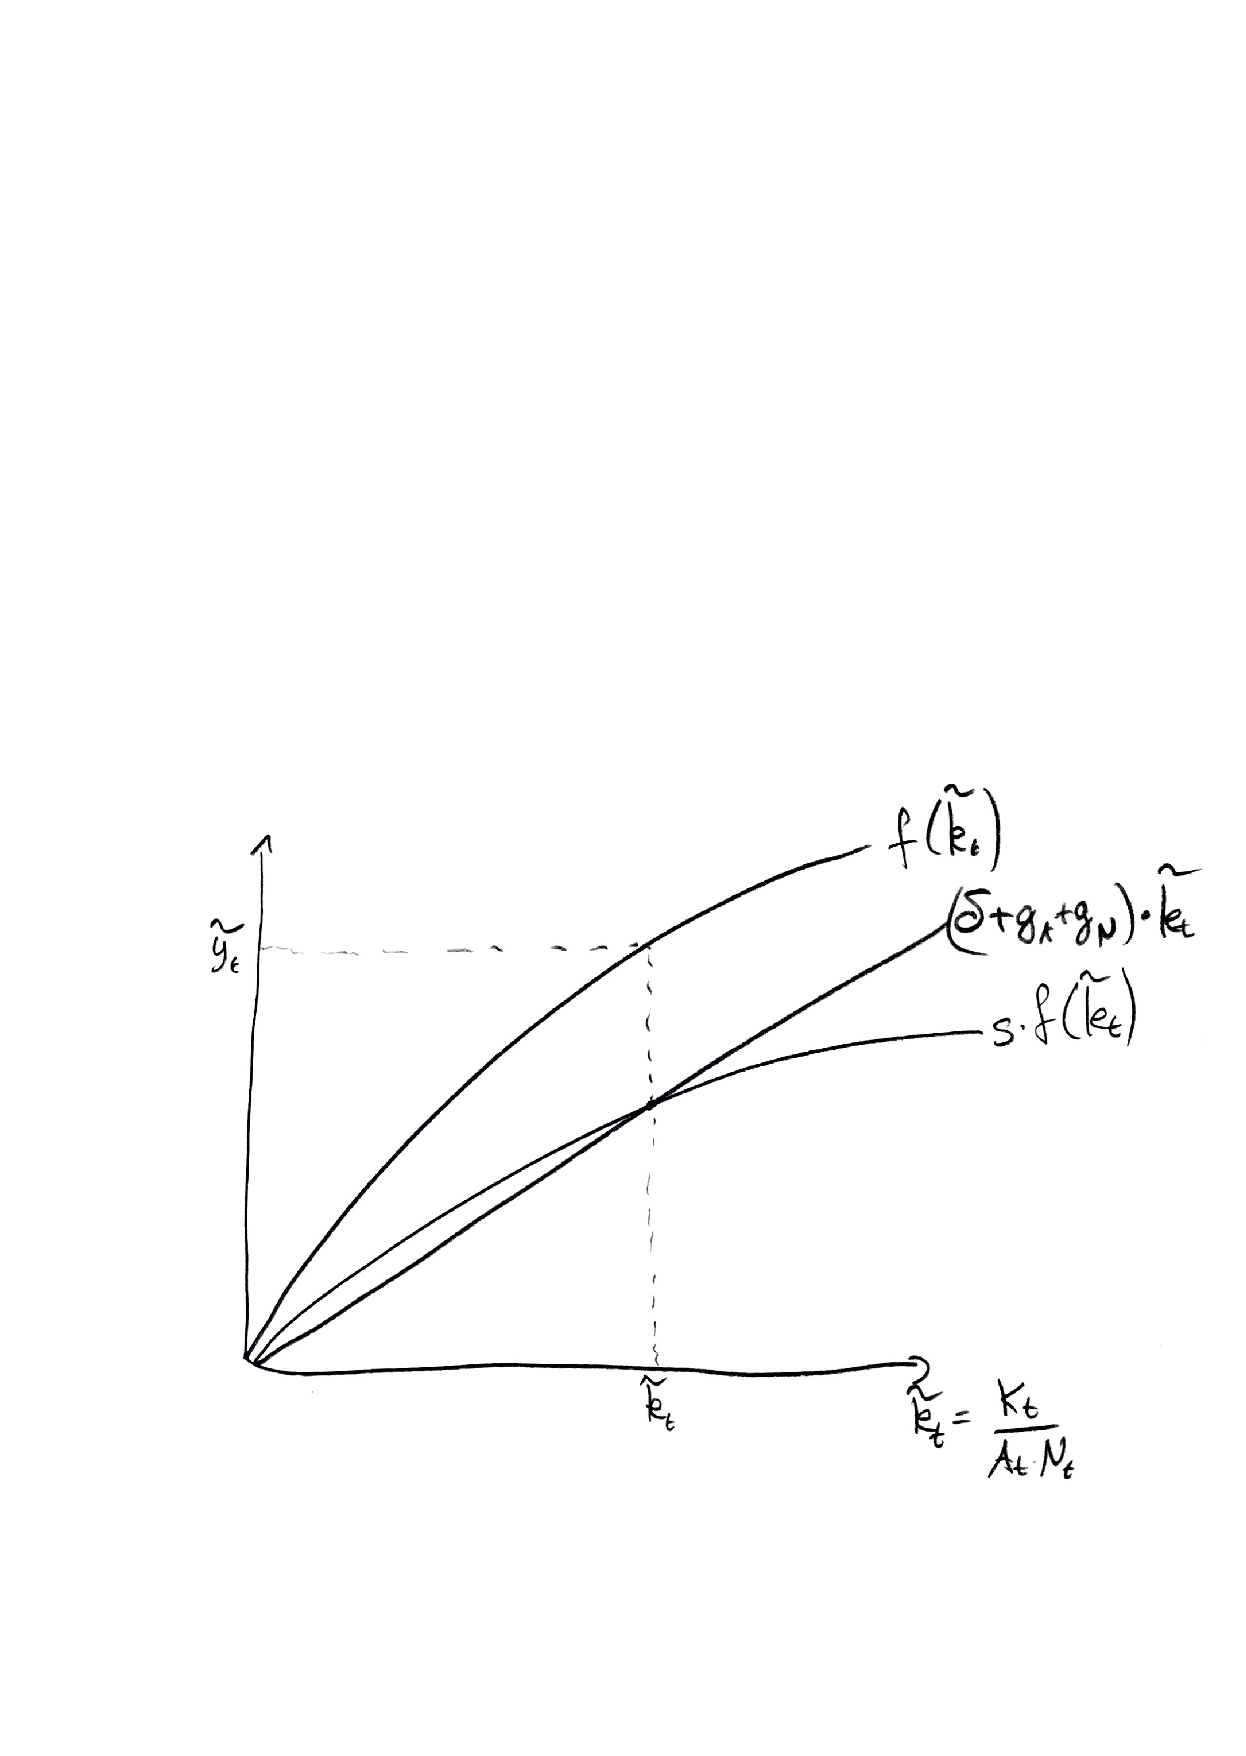
\includegraphics[width=\textwidth,keepaspectratio]{Bilder/Solow2.pdf}
  \item Wann verschiebe ich welche Kurve:
  \begin{itemize}
  \item Wachstum des technischen Fortschritt, Wachstum der Bev\"{o}lkerung oder Abschreibungsrate steigen: Drehung der Geraden $(\delta+g_A+g_N)\tilde{k}_t$ nach oben
  \item Sparquote steigt: $sf(\tilde{k}_t)$ verschiebt sich nach oben
  \end{itemize}
\end{itemize}
\end{enumerate}

Ein weiteres Konzept ist die sogenannte \emph{Goldene Regel} f\"{u}r die Sparquote: Die optimale Sparquote ist jene, bei der die Konsumm\"{o}glichkeiten einer Volkswirtschaft im steady state maximal werden. Wichtig: F\"{u}r die Goldene Regel muss sowohl die steady-state Bedingung als auch gelten, dass die Grenzproduktivit\"{a}t $f'(\tilde{k}_t)$ gleich $\delta+g_A+g_N$ ist:
\begin{align*}
  sf(\tilde{k}) &= (\delta + g_N + g_A)k\\
  f'(\tilde{k}) & = \delta + g_N + g_A
\end{align*}
Im einfachen Solow-Modell also:
\begin{align*}
  sf({k}) &= (\delta)k\\
  f'({k}) & = \delta
\end{align*}
Hinweis: Bei Cobb-Douglas-Produktionsfunktion ist die golden rule Sparquote $s^{**}=\alpha$!
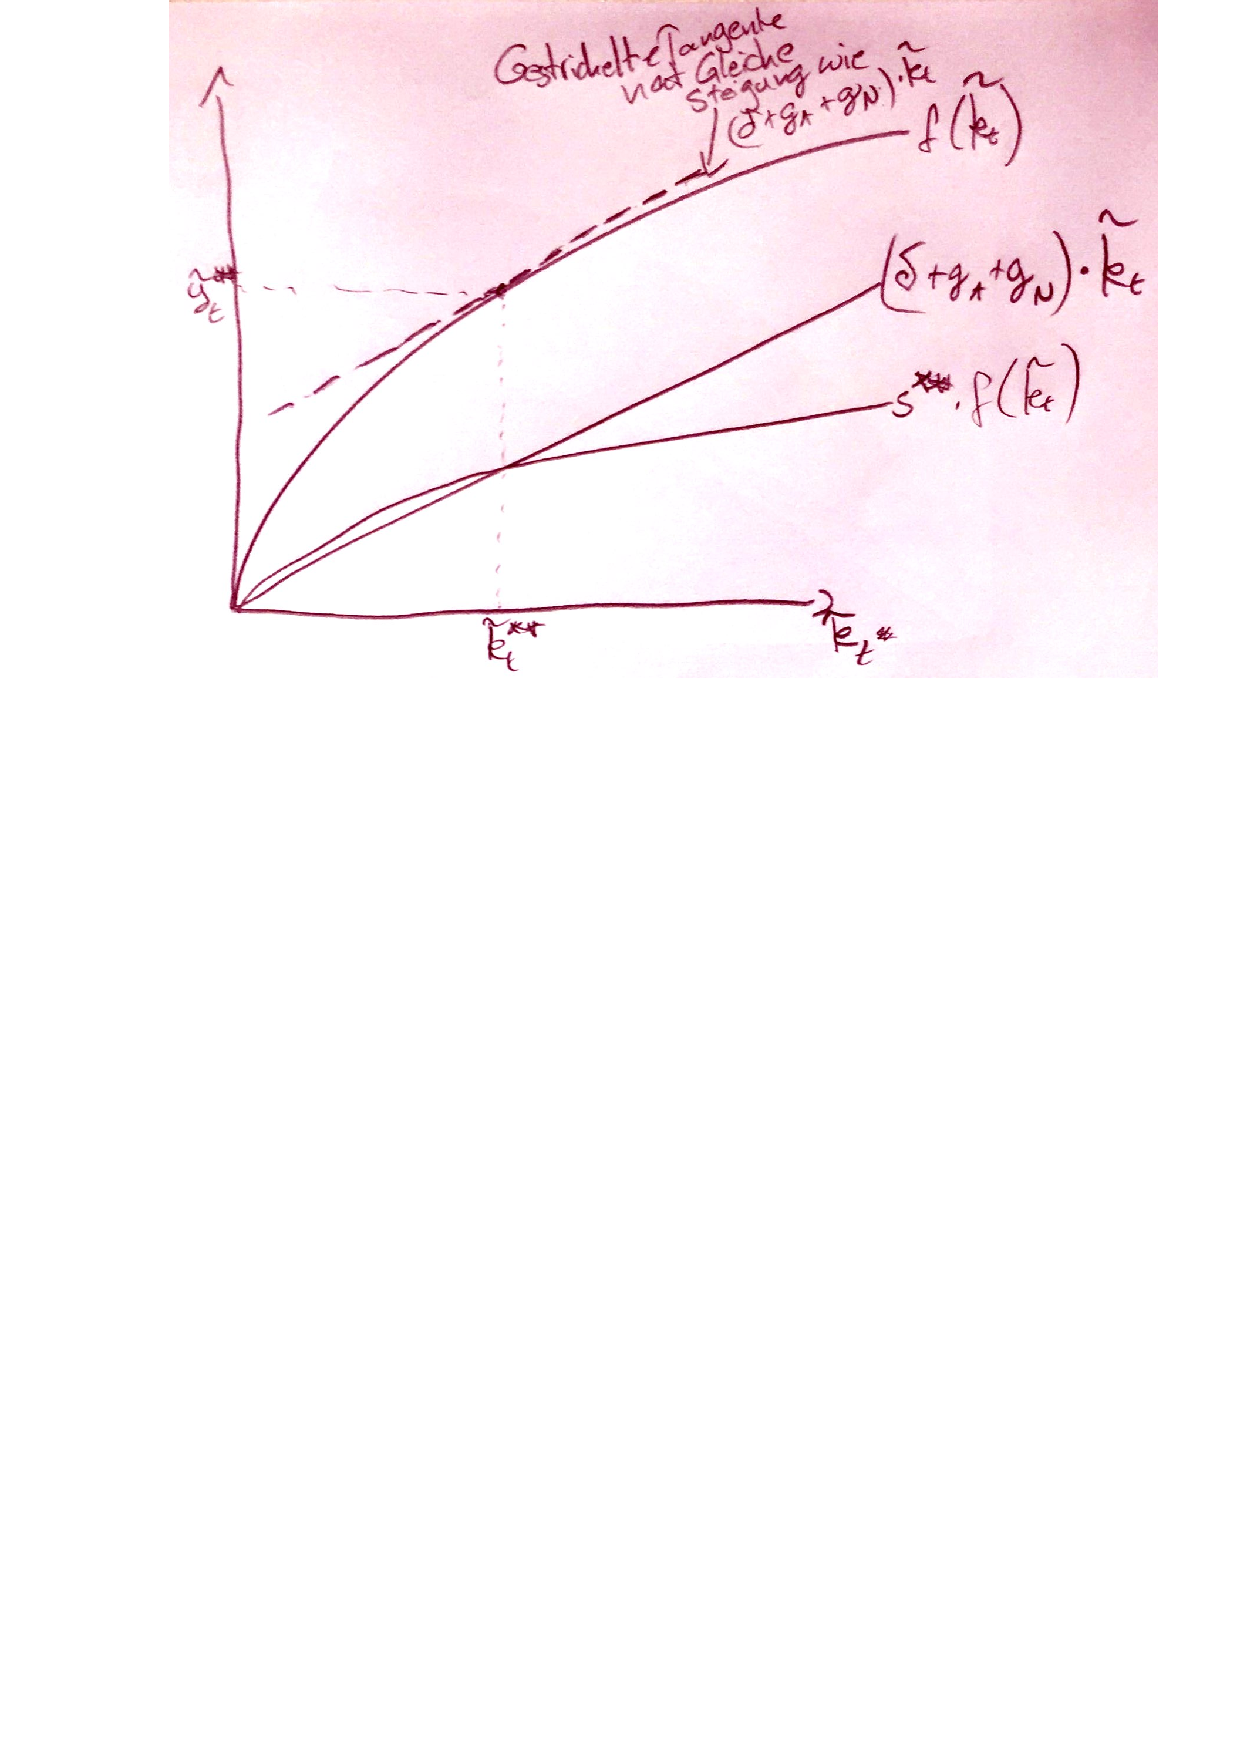
\includegraphics[width=\textwidth,keepaspectratio]{Bilder/SolowGoldenRule.pdf}
\subsection{Rechenaufgabe}
Einfaches Solow-Modell mit Bev\"{o}lkerungswachstum! Gegeben:\\
$y_t = \frac{Y_t}{N_t} = A k_t^{0.3} = f(k_t)$, $\frac{K}{Y}=\frac{k}{y}=3$, $g_Y=\frac{Y_{t+1}-Y_t}{Y_t} = 3\%$. Im einfachen Solow-Modell mit Bev\"{o}lkerungswachstum gilt: $g_Y=g_N$.
\begin{enumerate}[a)]
  \item $f'(k) = 0.3 \frac{A}{k^{0.7}}$. Wir wissen $\frac{y}{k}=\frac{A}{k^{0.7}} = \frac{1}{3}$. Einsetzen ergibt $f'(k) = 0.3\cdot \frac{1}{3} = 0.1.$
  \item Steady-State Bedingung: $sf(k)=(\delta + g_N)k$. Somit
  \begin{align*}
    s = \frac{(\delta+g_N)k}{y} = (\delta+g_N) \frac{k}{y} = (0.04+0.03)\cdot 3 = 0.21
  \end{align*}
  \item F\"{u}r goldene Regel muss f\"{u}r das Grenzprodukt des Kapitals gelten: $f'(k^{**})=\delta+g_N = 0.04+0.03 = 0.07$.
  \item Gesucht $s^{**}$. F\"{u}r goldene Regel muss gleichzeitig gelten:
  \begin{align*}
    1:& s^{**} f(k) = (\delta + g_N)k\\
    2:& f'(k) = \delta + g_N
  \end{align*}
  2 in 1:
  \begin{align*}
    s^{**} = \frac{f'(k)k}{f(k)} = \frac{\alpha A k^{\alpha-1}k}{Ak^\alpha} = \alpha
  \end{align*}
  Hier also: $s^{**} = 0.3$.
\end{enumerate}

\subsection{Zwei L\"{a}nder}
$n_A>n_B$ sonst alles gleich!
\begin{enumerate}
  \item Durchschnittliche Arbeitsproduktivit\"{a}t ist $Y/N$.\\ 
  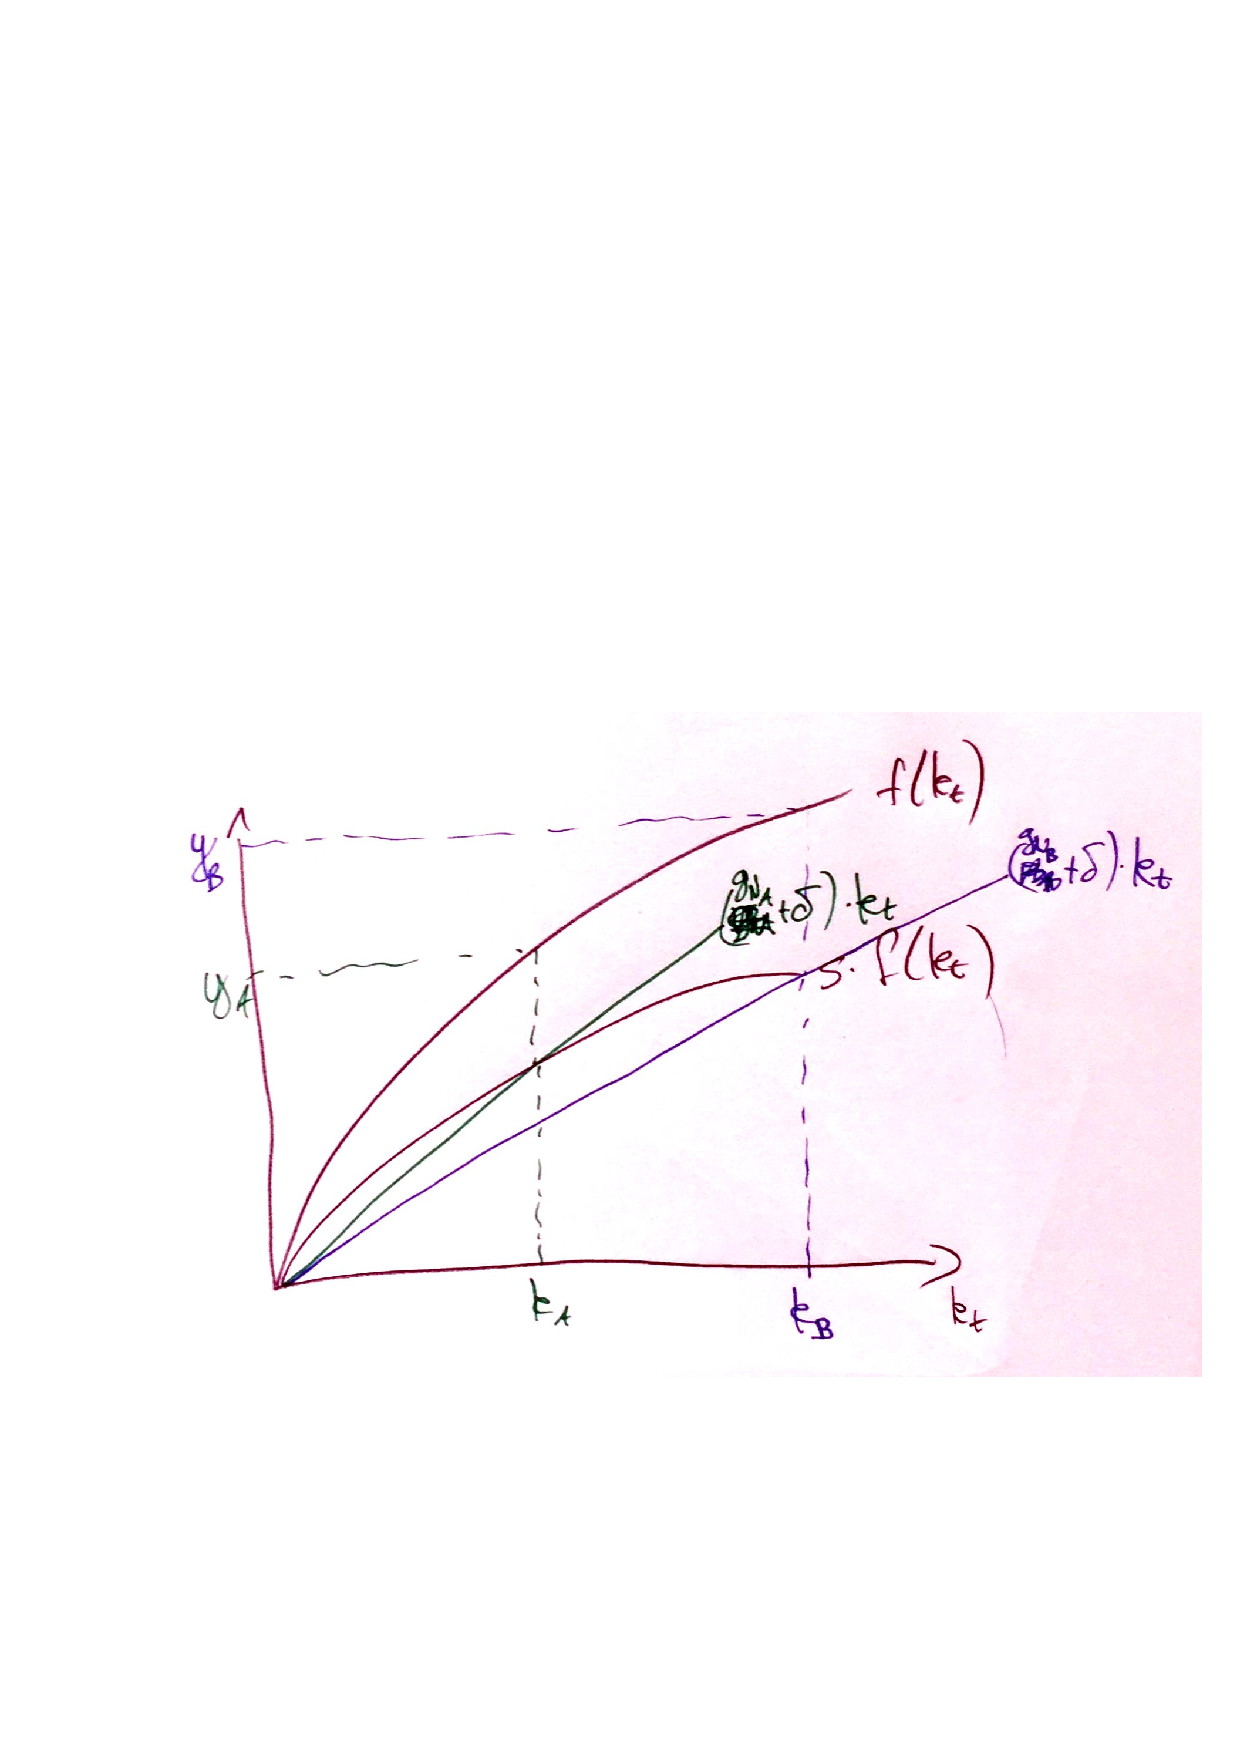
\includegraphics[width=\textwidth,keepaspectratio]{Bilder/Solow2Laender.pdf}
  Ergebnis: $y_B > y_A$.
  \item Wachstumsrate von $y$ im langfristigen Gleichgewicht ist Null! $g_y=0$, da $g_k=0$. Vorsicht: Niveaugr\"{o}{\ss}en $Y, K$ und $N$ wachsen mit der Bev\"{o}lkerungswachstumsrate.
\end{enumerate}

\subsection{Tropicana}
$\delta_T > \delta_S$, sonst alles Gleich. Frage: Wo ist die golden-rule Kapitalintensit\"{a}t gr\"{o}{\ss}er?\\
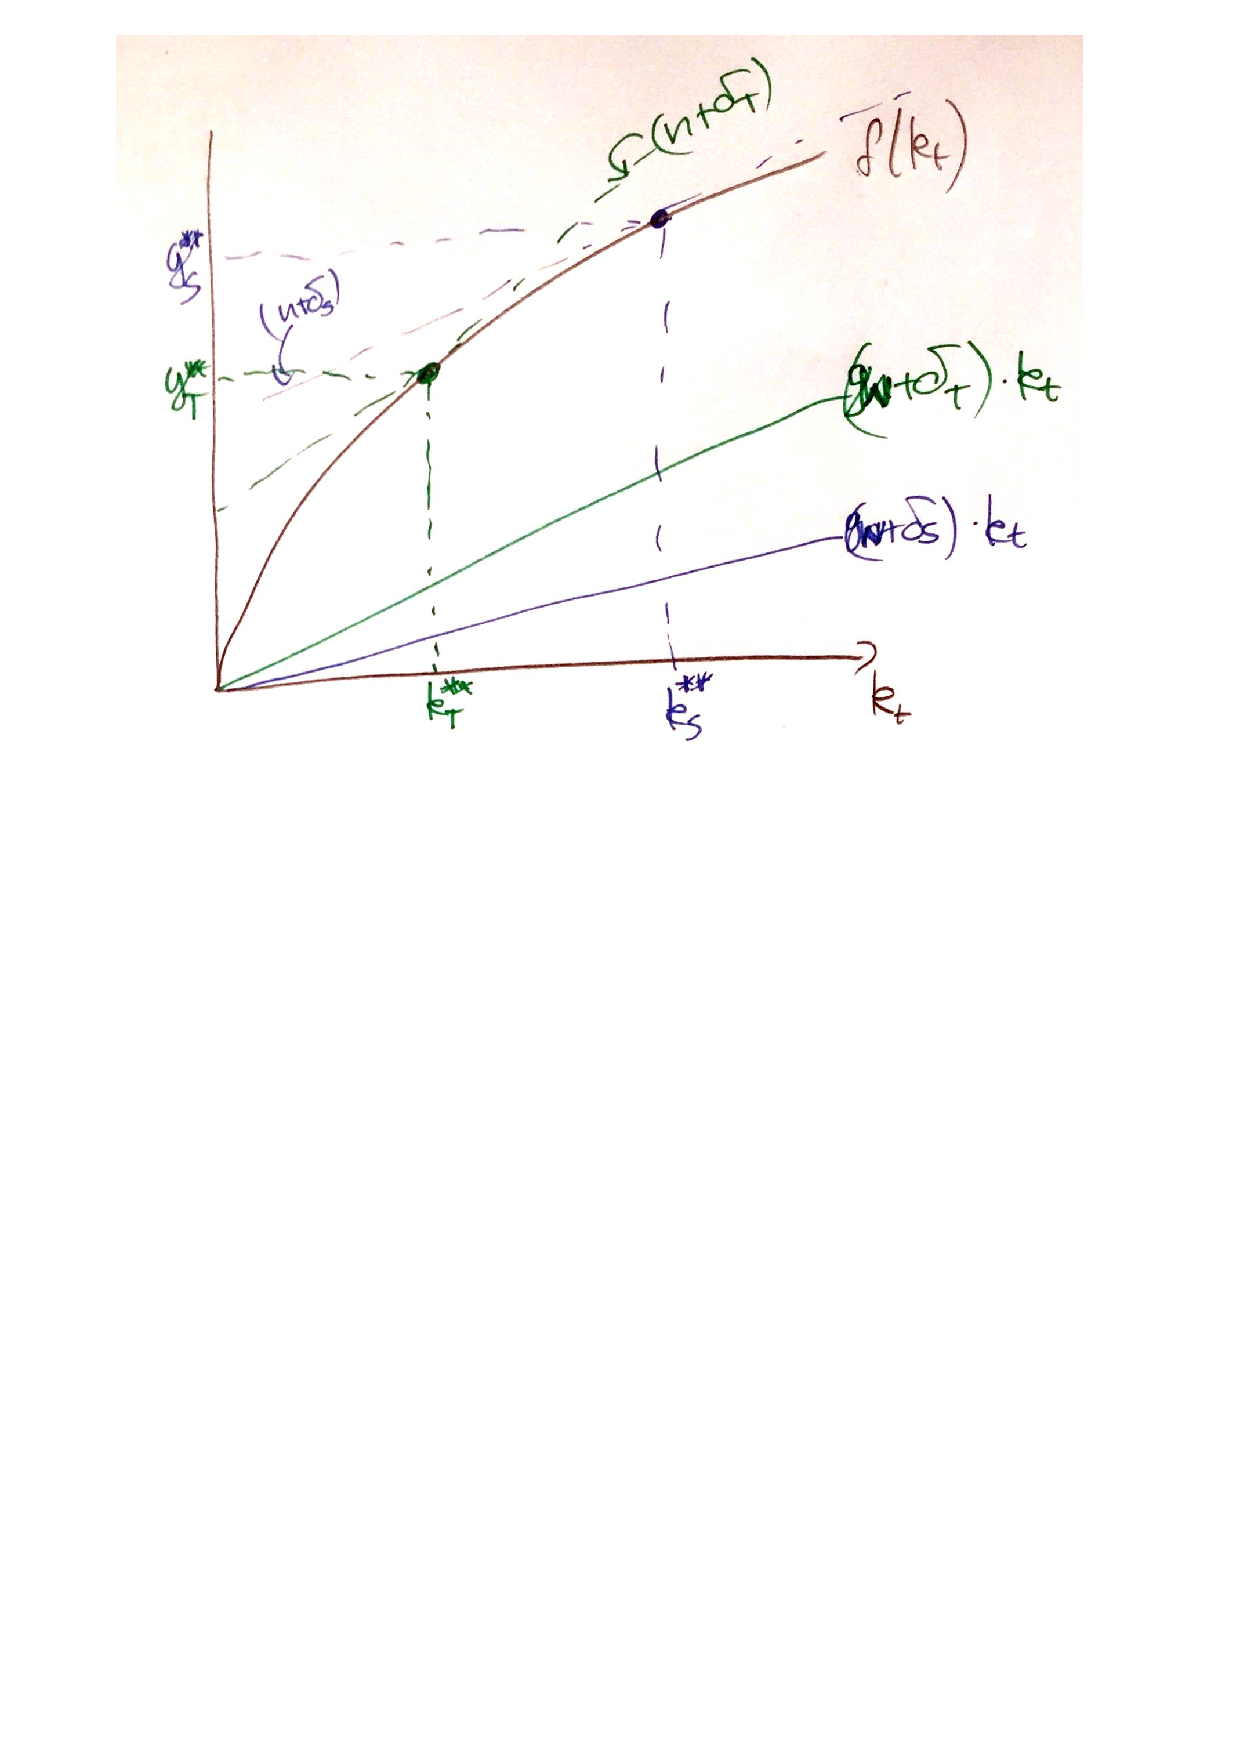
\includegraphics[width=\textwidth,keepaspectratio]{Bilder/SolowTropicana.pdf}
\subsection{China}
Wie \"{a}ndern sich $k$ und $y$?\\
\includegraphics[width=\textwidth,keepaspectratio]{Bilder/SolowChina.pdf}

%\subsection{Das allgemeine Keynesianische Modell bei festen Nominall\"{o}hnen}
%\begin{enumerate}[(a)]
%  \item Die Neoklassischen Synthese hat drei Punkte des Keynesianischen Nachfragesektors \"{u}bernommen:
%  \begin{itemize}
%    \item Abh\"{a}ngigkeit der Ersparnis/Konsum vom Einkommen
%    \item Nicht-Neutralit\"{a}t des Geldes: H\"{o}he der Zinsen beeinflusst die mit der Ersparnis identische Investition beeinflusst und \"{u}ber die ver\"{a}nderte Investition, verst\"{a}rkt durch den Multiplikator, das Gesamteinkommen der \"{O}konomie
%    \item Nominallohn kurzfristig fix, Preise sich nur langsam ver\"{a}ndernd
%  \end{itemize}
%  Aus der Neoklassik wird der Angebotssektor \"{u}bernommen:
%  \begin{itemize}
%    \item neoklassische Produktionsfunktion
%    \item neoklassischer Arbeitsmarkt (Nachfrage und Angebot auf dem Arbeitsmarkt abh\"{a}ngig vom Reallohn)
%  \end{itemize}
%    \includegraphics[width=0.5\textwidth]{Bilder/NeoklassischeSyntheseNormal.pdf}\\
%\item   Der Keynes-Effekt:\\
%    Durch ein sinkendes Preisniveau ist das reale Geldangebot gr\"{o}{\ss}er als die Geldnachfrage (Transaktions- und Spekulationskasse). Haushalte und Unternehmen versuchen durch eine h\"{o}here Nachfrage am Wertpapiermarkt die \"{u}berh\"{o}hte Geldhaltung wieder abzubauen. Dabei kommt es mit der h\"{o}heren Nachfrage zu einem Anstieg der Wertpapierkurse und daraus resultierend zu sinkenden Zinsen. Bei sinkenden Zinsen steigen Investition, G\"{u}ternachfrage und Besch\"{a}ftigung gem\"{a}{\ss} dem Multiplikatorprozess. Keyens-Effekt wirkt jedoch nicht in der Investitions-oder Liquidit\"{a}tsfalle.
%
%\item Gleichgewicht bei Unterbesch\"{a}ftigung\\
%\includegraphics[width=\textwidth]{Bilder/NeoklassischeSyntheseUnterbeschaftigung.pdf}\\
%\begin{itemize}
%  \item Gleichgewicht auf Kapital-und Geldmarkt (IS/LM)
%  \item Angebots\"{u}berschuss (A\"{U}) auf Arbeits-und G\"{u}termarkt
%  \item Reallohnsenkung weder n\"{o}tig noch wirksam
%  \item Unternehmen sind auf dem G\"{u}termarkt rationiert => Arbeitsnachfrage gilt hier nicht
%  \item Arbeitnehmer sind auf dem Arbeitsmarkt rationiert
%\end{itemize}
%Denkbare Auswege:
%\begin{itemize}
%\item sinkende Preise und Nominall\"{o}hne (Bewegung auf AD nach rechts) --> Keynes-Effekt!
%\item expansive Geld-oder Fiskalpolitik (Verschiebung von AD nach rechts)
%\end{itemize}
%
%\item
%\begin{enumerate}[(i)]
%  \item Investitionsfalle\\ \includegraphics[width=\textwidth]{Bilder/NeoklassischeSyntheseInvest.pdf}\\
%  \item Liquidit\"{a}tsfalle \\ \includegraphics[width=\textwidth]{Bilder/NeoklassischeSyntheseLiquid.pdf}\\
%\end{enumerate}
%Auswege bei beiden: Fiskalpolitik
%
%\item \includegraphics[width=\textwidth]{Bilder/NeoklassischeSyntheseFixLohnGeld.pdf}\\
%Bei starren Nominall\"{o}hnen ist die Geldpolitik in der Lage, durch Inflation, das neoklassische Gleichgewicht zu erreichen.
%
%\end{enumerate}



%\section{Lindberg und Robertson-Lag}
%\begin{enumerate}
%  \item Lags
%  \begin{itemize}
%  \item Lundberg: Fokus auf Verz\"{o}gerung zwischen \"{A}nderung der Nachfrage und Antwort des Outputs
%  \item Robertson: Fokus auf Verz\"{o}gerung im Konsum aufgrund einer Einkommens\"{a}nderung
%  \end{itemize}
%  \item \begin{enumerate}[a)]
%      \item \begin{align*}
%        Y = C+I+G = C_{aut} + cY + I_{aut}+ G_{aut} \Rightarrow Y^* = \frac{1-c}(C_{aut}+I_{aut}+G_{aut})= \frac{1}{1-0.5}(50+50+100)=400
%      \end{align*}
%  \item Lundberg-Lag: Produktion richtet sich nach Gesamtnachfrage der Vorperiode, d.h.
%  \begin{align*}
%    Y_t = Y_t^s = Y_{t-1}^d = C_{t-1} + I_{t-1}+G_{t-1}, C_t = C_{aut}+c Y_t
%  \end{align*}
%  Robertson-Lag: Konsum richtet sich nach Einkommen der Vorperiode
%  \begin{align*}
%    C_t = C_{aut} + c Y_{t-1}, Y_t = C_t + I_t + G_t
%  \end{align*}
%  \item in $t+1:$ $G_{aut}=150$,
%  Neues GG: $Y^* = \frac{1}{1-0.5}(50+50+150) = 500, C^* = 300$\\
%  Lundberg-Lag\\
%  \begin{tabular}{|c|c|c|c|c|}
%    \hline
%    % after \\: \hline or \cline{col1-col2} \cline{col3-col4} ...
%      & $C_t=C_{aut}+c Y_t$ & $I_{aut}$ & $G_t$ & $Y_t =C_{t-1}+I_{t-1}+G_{t-1}$ \\\hline
%    0 & 250 & 50 & 100 &  \\
%    1 & 250 & 50 & 150 & 400 \\
%    2 & 275 & 50 & 150 & 450 \\
%    3 & 287,5& 50 & 150 & 475 \\
%    $\vdots$ & $\vdots$ & $\vdots$ & $\vdots$ & $\vdots$ \\
%    $\infty$ & 300 & 50 & 150 & 500 \\
%    \hline
%  \end{tabular}\\
%
%  Robertson-Lag\\
%    \begin{tabular}{|c|c|c|c|c|}
%    \hline
%    % after \\: \hline or \cline{col1-col2} \cline{col3-col4} ...
%      & $C_t=C_{aut}+c Y_{t-1}$ & $I_{aut}$ & $G_t$ & $Y_t =C_{t}+I_{t}+G_{t}$ \\\hline
%    0 & 250 & 50 & 100 & 400 \\
%    1 & 250 & 50 & 150 & 450 \\
%    2 & 275 & 50 & 150 & 475 \\
%    3 & 287,5& 50 & 150 & 487,5 \\
%    $\vdots$ & $\vdots$ & $\vdots$ & $\vdots$ & $\vdots$ \\
%    $\infty$ & 300 & 50 & 150 & 500 \\
%    \hline
%  \end{tabular}
%  \end{enumerate}
%
%\end{enumerate}
%
%\section{Hick'sche Wachstumsmodell}
%\begin{enumerate}[a)]
%  \item Konjunktur-Modell\\
%  \begin{enumerate}[(1)]
%  \item Idee: Konsumgleichung mit Robertson-Lag (Konsumverz\"{o}gerung h\"{a}ngt ab von EK der Vorperiode)\\
%  \item
%  \Tree [.{Investitionen} [.{Bestandteil der Nachfrage} ] [.{Wachstum des Kapitalstocks} [{Investitionsentscheidung\\bzgl. des angestrebten Kapitalstocks} Angebot ] ]]\\
%  Annahme: Es gibt effizienten Kapitalstock --> Investitionen werden \"{u}ber diesen optimalen Kapitalstock bestimmt (nicht \"{u}ber Zins)
%  \begin{align*}
%    I_t = K_{t} - K_{t-1} = I_{aut} + a(Y_{t-1}-Y_{t-2})
%  \end{align*}
%  Intuitiver Grund: Angestrebter Kapitalstock h\"{a}ngt von der angestrebten Produktion und damit von der erwarteten Nachfrage ab: $Y^d \uparrow \rightarrow K_p \uparrow \rightarrow I \uparrow$.\\
%  Wichtig: Investitionen h\"{a}ngen nicht vom Niveau des EKs ab, sonder vom Wachstum des EKs!\\
%  \item G\"{u}termarkt-GG
%  \end{enumerate}
%  \item Warum Akzelerator?\\
%  EK steigt, angestrebter Kapitalstock steigt, Investitionen steigen, Nachfrage steigt, EK steigt, angestrebter Kapitalstock steigt $\Rightarrow$ EIMALIGER AKZELERATIONSPROZESS, da Wachstumsabh\"{a}ngig
%  \item \begin{enumerate}[a)]
%    \item $Y^*=400$
%    \item
%        \begin{tabular}{|c|c|c|c|c|c|}
%    \hline
%    % after \\: \hline or \cline{col1-col2} \cline{col3-col4} ...
%      & $C_t=C_{aut}+c Y_{t-1}$ & $I_{aut}$ & $I_{ind} = Y_t - Y_{t-1}$& $G_t$ & $Y_t =C_{t}+I_{t}+G_{t}$ \\\hline
%    1 & 250 & 50 & 0 & 100 & 400 \\
%    2 & 250 & 50 & 0 & 100 & 400 \\
%    3 & 250 & 50 & 0 & 100 & 400 \\
%    4 & 250 & 50 & 0 & 150 & 450 \\
%    5 & 275 & 50 & 50 & 100 & 475 \\
%    6 & 287,5& 50& 25 & 100 & 462,5 \\
%    7 & 281,25& 50& -12.5 & 100 & 418.75 \\
%    8 & 259,375& 50& -43.75 & 100 & <400 \\
%    $\vdots$ & $\vdots$ & $\vdots$ & $\vdots$ & $\vdots$ &\vdots\\
%    \hline
%  \end{tabular}\\
%Ek-Senkung in periode 6 aufgrund Akzelerator.
%\item \begin{itemize}
%  \item $v<1:$ abnehmende Schwingung
%  \item $v=1:$ Chance auf stabile Schwingung
%  \item $v>1:$ sehr gro{\ss}e Schwingungen
%\end{itemize}
%  \end{enumerate}
%\end{enumerate}

\end{document}



%%%%%%%%%%% AUSSORTIERT%%%%%%%%%%%%%%


